%!TEX program = xelatex 
%!TEX encoding = ISO-8859-1
%%%%%%%%%%%%%%%%%%%%%%%%%%%%%%%%%%%%%%%%%
% The Legrand Orange Book
% LaTeX Template
% Version 2.3 (8/8/17)
%
% This template has been downloaded from:
% http://www.LaTeXTemplates.com
%
% Original author:
% Mathias Legrand (legrand.mathias@gmail.com) with modifications by:
% Vel (vel@latextemplates.com)
%
% License:
% CC BY-NC-SA 3.0 (http://creativecommons.org/licenses/by-nc-sa/3.0/)
%
% Compiling this template:
% This template uses biber for its bibliography and makeindex for its index.
% When you first open the template, compile it from the command line with the 
% commands below to make sure your LaTeX distribution is configured correctly:
%
% 1) pdflatex main
% 2) makeindex main.idx -s StyleInd.ist
% 3) biber main
% 4) pdflatex main x 2
%
% After this, when you wish to update the bibliography/index use the appropriate
% command above and make sure to compile with pdflatex several times 
% afterwards to propagate your changes to the document.
%
% This template also uses a number of packages which may need to be
% updated to the newest versions for the template to compile. It is strongly
% recommended you update your LaTeX distribution if you have any
% compilation errors.
%
% Important note:
% Chapter heading images should have a 2:1 width:height ratio,
% e.g. 920px width and 460px height.
%
%%%%%%%%%%%%%%%%%%%%%%%%%%%%%%%%%%%%%%%%%

%----------------------------------------------------------------------------------------
%   PACKAGES AND OTHER DOCUMENT CONFIGURATIONS
%----------------------------------------------------------------------------------------

\documentclass[11pt,fleqn]{book} % Default font size and left-justified equations

%----------------------------------------------------------------------------------------

%!TEX program = xelatex
%!TEX root = Algebra_Linear.tex
%%%%%%%%%%%%%%%%%%%%%%%%%%%%%%%%%%%%%%%%%
% The Legrand Orange Book
% Structural Definitions File
% Version 2.0 (9/2/15)
%
% Original author:
% Mathias Legrand (legrand.mathias@gmail.com) with modifications by:
% Vel (vel@latextemplates.com)
% 
% This file has been downloaded from:
% http://www.LaTeXTemplates.com
%
% License:
% CC BY-NC-SA 3.0 (http://creativecommons.org/licenses/by-nc-sa/3.0/)
%
%%%%%%%%%%%%%%%%%%%%%%%%%%%%%%%%%%%%%%%%%

%----------------------------------------------------------------------------------------
%	VARIOUS REQUIRED PACKAGES AND CONFIGURATIONS
%----------------------------------------------------------------------------------------

\usepackage[top=3cm,bottom=3cm,left=3cm,right=3cm,headsep=10pt,a4paper]{geometry} % Page margins

\usepackage{graphicx} % Required for including pictures
\graphicspath{{Pictures/}} % Specifies the directory where pictures are stored

\usepackage{ccicons} %ícones creative commons

\usepackage{amssymb,amsmath,amsfonts,amsthm,amstext}

\usepackage{enumitem}

\usepackage{lipsum} % Inserts dummy text

\usepackage{tikz} % Required for drawing custom shapes

\usepackage[brazil]{babel}

\usepackage{multicol}

\usepackage{gauss}

\usepackage{enumitem} % Customize lists
\setlist{nolistsep} % Reduce spacing between bullet points and numbered lists

\usepackage{booktabs} % Required for nicer horizontal rules in tables

\usepackage{xcolor} % Required for specifying colors by name
\definecolor{ocre}{RGB}{243,102,25} % Define the orange color used for highlighting throughout the book

%----------------------------------------------------------------------------------------
%	FONTS
%----------------------------------------------------------------------------------------

\usepackage{avant} % Use the Avantgarde font for headings
%\usepackage{times} % Use the Times font for headings
\usepackage{mathptmx} % Use the Adobe Times Roman as the default text font together with math symbols from the Sym­bol, Chancery and Com­puter Modern fonts

\usepackage{microtype} % Slightly tweak font spacing for aesthetics
\usepackage[utf8]{inputenc} % Required for including letters with accents
\usepackage[T1]{fontenc} % Use 8-bit encoding that has 256 glyphs

%----------------------------------------------------------------------------------------
%	BIBLIOGRAPHY AND INDEX
%----------------------------------------------------------------------------------------

% \usepackage[style=numeric,citestyle=numeric,sorting=nyt,sortcites=true,autopunct=true,babel=hyphen,hyperref=true,abbreviate=false,backref=true,backend=biber]{biblatex}
% \addbibresource{bibliography.bib} % BibTeX bibliography file
% \defbibheading{bibempty}{}

\usepackage{calc} % For simpler calculation - used for spacing the index letter headings correctly
\usepackage{makeidx} % Required to make an index
\makeindex % Tells LaTeX to create the files required for indexing

%----------------------------------------------------------------------------------------
%	MAIN TABLE OF CONTENTS
%----------------------------------------------------------------------------------------

\usepackage{titletoc} % Required for manipulating the table of contents

\contentsmargin{0cm} % Removes the default margin

% Part text styling
\titlecontents{part}[0cm]
{\addvspace{20pt}\centering\large\bfseries}
{}
{}
{}

% Chapter text styling
\titlecontents{chapter}[1.25cm] % Indentation
{\addvspace{12pt}\large\sffamily\bfseries} % Spacing and font options for chapters
{\color{ocre!60}\contentslabel[\Large\thecontentslabel]{1.25cm}\color{ocre}} % Chapter number
{\color{ocre}}  
{\color{ocre!60}\normalsize\;\titlerule*[.5pc]{.}\;\thecontentspage} % Page number

% Section text styling
\titlecontents{section}[1.25cm] % Indentation
{\addvspace{3pt}\sffamily\bfseries} % Spacing and font options for sections
{\contentslabel[\thecontentslabel]{1.25cm}} % Section number
{}
{\hfill\color{black}\thecontentspage} % Page number
[]

% Subsection text styling
\titlecontents{subsection}[1.25cm] % Indentation
{\addvspace{1pt}\sffamily\small} % Spacing and font options for subsections
{\contentslabel[\thecontentslabel]{1.25cm}} % Subsection number
{}
{\ \titlerule*[.5pc]{.}\;\thecontentspage} % Page number
[]

% List of figures
\titlecontents{figure}[0em]
{\addvspace{-5pt}\sffamily}
{\thecontentslabel\hspace*{1em}}
{}
{\ \titlerule*[.5pc]{.}\;\thecontentspage}
[]

% List of tables
\titlecontents{table}[0em]
{\addvspace{-5pt}\sffamily}
{\thecontentslabel\hspace*{1em}}
{}
{\ \titlerule*[.5pc]{.}\;\thecontentspage}
[]

%----------------------------------------------------------------------------------------
%	MINI TABLE OF CONTENTS IN PART HEADS
%----------------------------------------------------------------------------------------

% Chapter text styling
\titlecontents{lchapter}[0em] % Indenting
{\addvspace{15pt}\large\sffamily\bfseries} % Spacing and font options for chapters
{\color{ocre}\contentslabel[\Large\thecontentslabel]{1.25cm}\color{ocre}} % Chapter number
{}  
{\color{ocre}\normalsize\sffamily\bfseries\;\titlerule*[.5pc]{.}\;\thecontentspage} % Page number

% Section text styling
\titlecontents{lsection}[0em] % Indenting
{\sffamily\small} % Spacing and font options for sections
{\contentslabel[\thecontentslabel]{1.25cm}} % Section number
{}
{}

% Subsection text styling
\titlecontents{lsubsection}[.5em] % Indentation
{\normalfont\footnotesize\sffamily} % Font settings
{}
{}
{}

%----------------------------------------------------------------------------------------
%	PAGE HEADERS
%----------------------------------------------------------------------------------------

\usepackage{fancyhdr} % Required for header and footer configuration

\pagestyle{fancy}
\renewcommand{\chaptermark}[1]{\markboth{\sffamily\normalsize\bfseries\chaptername\ \thechapter.\ #1}{}} % Chapter text font settings
\renewcommand{\sectionmark}[1]{\markright{\sffamily\normalsize\thesection\hspace{5pt}#1}{}} % Section text font settings
\fancyhf{} \fancyhead[LE,RO]{\sffamily\normalsize\thepage} % Font setting for the page number in the header
\fancyhead[LO]{\rightmark} % Print the nearest section name on the left side of odd pages
\fancyhead[RE]{\leftmark} % Print the current chapter name on the right side of even pages
\renewcommand{\headrulewidth}{0.5pt} % Width of the rule under the header
\addtolength{\headheight}{2.5pt} % Increase the spacing around the header slightly
\renewcommand{\footrulewidth}{0pt} % Removes the rule in the footer
\fancypagestyle{plain}{\fancyhead{}\renewcommand{\headrulewidth}{0pt}} % Style for when a plain pagestyle is specified

% Removes the header from odd empty pages at the end of chapters
\makeatletter
\renewcommand{\cleardoublepage}{
\clearpage\ifodd\c@page\else
\hbox{}
\vspace*{\fill}
\thispagestyle{empty}
\newpage
\fi}

%----------------------------------------------------------------------------------------
%	THEOREM STYLES
%----------------------------------------------------------------------------------------

\usepackage{amsmath,amsfonts,amssymb,amsthm} % For math equations, theorems, symbols, etc

\newcommand{\intoo}[2]{\mathopen{]}#1\,;#2\mathclose{[}}
\newcommand{\ud}{\mathop{\mathrm{{}d}}\mathopen{}}
\newcommand{\intff}[2]{\mathopen{[}#1\,;#2\mathclose{]}}
\newtheorem{notation}{Notation}[chapter]
\newtheoremstyle{dotless}{}{}{\itshape}{}{\bfseries}{}{ }{}
\theoremstyle{dotless}
\newtheorem*{solucao}{Solu{\c c}{\~a}o:}

% Boxed/framed environments
\newtheoremstyle{ocrenumbox}% % Theorem style name
{0pt}% Space above
{0pt}% Space below
{\normalfont}% % Body font
{}% Indent amount
{\small\bf\sffamily\color{ocre}}% % Theorem head font
{\;}% Punctuation after theorem head
{0.25em}% Space after theorem head
{\small\sffamily\color{ocre}\thmname{#1}\nobreakspace\thmnumber{\@ifnotempty{#1}{}\@upn{#2}}% Theorem text (e.g. Theorem 2.1)
\thmnote{\nobreakspace\the\thm@notefont\sffamily\bfseries\color{black}---\nobreakspace#3.}} % Optional theorem note
\renewcommand{\qedsymbol}{$\blacksquare$}% Optional qed square

\newtheoremstyle{blacknumex}% Theorem style name
{5pt}% Space above
{5pt}% Space below
{\normalfont}% Body font
{} % Indent amount
{\small\bf\sffamily}% Theorem head font
{\;}% Punctuation after theorem head
{0.25em}% Space after theorem head
{\small\sffamily{\tiny\ensuremath{\blacksquare}}\nobreakspace\thmname{#1}\nobreakspace\thmnumber{\@ifnotempty{#1}{}\@upn{#2}}% Theorem text (e.g. Theorem 2.1)
\thmnote{\nobreakspace\the\thm@notefont\sffamily\bfseries---\nobreakspace#3.}}% Optional theorem note

\newtheoremstyle{blacknumbox} % Theorem style name
{0pt}% Space above
{0pt}% Space below
{\normalfont}% Body font
{}% Indent amount
{\small\bf\sffamily}% Theorem head font
{\;}% Punctuation after theorem head
{0.25em}% Space after theorem head
{\small\sffamily\thmname{#1}\nobreakspace\thmnumber{\@ifnotempty{#1}{}\@upn{#2}}% Theorem text (e.g. Theorem 2.1)
\thmnote{\nobreakspace\the\thm@notefont\sffamily\bfseries---\nobreakspace#3.}}% Optional theorem note

% Non-boxed/non-framed environments
\newtheoremstyle{ocrenum}% % Theorem style name
{5pt}% Space above
{5pt}% Space below
{\normalfont}% % Body font
{}% Indent amount
{\small\bf\sffamily\color{ocre}}% % Theorem head font
{\;}% Punctuation after theorem head
{0.25em}% Space after theorem head
{\small\sffamily\color{ocre}\thmname{#1}\nobreakspace\thmnumber{\@ifnotempty{#1}{}\@upn{#2}}% Theorem text (e.g. Theorem 2.1)
\thmnote{\nobreakspace\the\thm@notefont\sffamily\bfseries\color{black}---\nobreakspace#3.}} % Optional theorem note
\renewcommand{\qedsymbol}{$\blacksquare$}% Optional qed square
\makeatother

% Defines the theorem text style for each type of theorem to one of the three styles above
\newcounter{dummy} 
\numberwithin{dummy}{section}
\theoremstyle{ocrenumbox}
\newtheorem{teoremaT}[dummy]{Teorema}
\newtheorem{notacao}{Nota\c{c}\~ao}[section]
\newtheorem{problema}{Problema}[chapter]
\newtheorem{exercicio}{Exercício}[chapter]
\theoremstyle{blacknumex}
\newtheorem{exemplo}{Exemplo}[chapter]
\newtheorem{exemplos}{Exemplos}[chapter]
\newtheorem{observacao}{Observaçao}[chapter]
\newtheorem{observacoes}{Observações}[chapter]
\newtheorem{nota}{Nota}[chapter]
\theoremstyle{blacknumbox}
\newtheorem{vocabulary}{Vocabulary}[chapter]
\newtheorem{definicaoT}{Definição}[section]
\newtheorem{definicoesT}{Definições}[section]
\newtheorem{corolarioT}[dummy]{Corolário}
\theoremstyle{ocrenum}
\newtheorem{proposicao}[dummy]{Proposição}
\newtheorem{lema}[dummy]{Lema}
\newtheorem{propriedades}{Propriedades}[section]
\newenvironment{prova}[1][Prova]{\noindent\textbf{#1:} }{\qedsymbol}%{\ \rule{0.5em}{0.5em}}

%----------------------------------------------------------------------------------------
%	MATH COMMANDS
%----------------------------------------------------------------------------------------


\newcommand{\n}{\mathbb{N}}
\newcommand{\z}{\mathbb{Z}}
\newcommand{\rac}{\mathbb{Q}}
\newcommand{\dom}{{\rm dom\,}}
\newcommand{\im}{{\rm Im\,}}
\newcommand{\aut}{{\rm Aut\,}}
\newcommand{\cp}[1]{\mathbb{#1}}
\newcommand{\sub}{\subseteq}
\newcommand{\real}{\mathbb{R}}
\newcommand{\complex}{\mathbb{C}}
\newcommand{\lap}[1]{\mathcal{L}\left\{#1\right\}}
\newcommand{\lapi}[1]{\mathcal{L}^{-1}\left\{#1\right\}}
\newcommand{\se}[1]{\displaystyle\sum_{n = 1}^\infty{#1}}
\newcommand{\dlim}[2]{\displaystyle\lim_{#1\rightarrow #2}}
\newcommand{\slim}{\displaystyle\lim_{n \rightarrow \infty}}
\newcommand{\seq}[1]{\{{#1_n\}}}
\newcommand{\seg}[1]{\displaystyle\sum_{n = 1}^\infty{#1_n}}
\newcommand{\sei}[2]{\displaystyle\sum_{#1}^\infty{#2}}
\newcommand{\sepc}[3]{\displaystyle\sum_{#1}^\infty{#2(x - #3)^n}}
\newcommand{\imp}[3]{\displaystyle\int_{#1}^{+\infty}{#3}{d #2}}
\newcommand{\dint}[4]{\displaystyle\int_{#1}^{#2}{#4}{d#3}}
\newcommand{\inti}[2]{\displaystyle\int{#1}{d#2}}
\newcommand{\norma}[1]{\left\lVert#1\right\rVert}
\newcommand{\flim}[1]{\displaystyle\lim_{#1\rightarrow \infty}}
\renewcommand{\sin}{{\rm sen\,}}
\renewcommand{\tan}{{\rm tg\,}}
\renewcommand{\csc}{{\rm cossec\,}}
\renewcommand{\cot}{{\rm cotg\,}}
\renewcommand{\sinh}{{\rm senh\,}}
\newcommand\T{\rule{0pt}{2.6ex}} 


%----------------------------------------------------------------------------------------
%	DEFINITION OF COLORED BOXES
%----------------------------------------------------------------------------------------

\RequirePackage[framemethod=default]{mdframed} % Required for creating the theorem, definition, exercise and corollary boxes

% Theorem box
\newmdenv[skipabove=7pt,
skipbelow=7pt,
backgroundcolor=black!5,
linecolor=ocre,
innerleftmargin=5pt,
innerrightmargin=5pt,
innertopmargin=5pt,
leftmargin=0cm,
rightmargin=0cm,
innerbottommargin=5pt]{tBox}

% Exercise box	  
\newmdenv[skipabove=7pt,
skipbelow=7pt,
rightline=false,
leftline=true,
topline=false,
bottomline=false,
backgroundcolor=ocre!10,
linecolor=ocre,
innerleftmargin=5pt,
innerrightmargin=5pt,
innertopmargin=5pt,
innerbottommargin=5pt,
leftmargin=0cm,
rightmargin=0cm,
linewidth=4pt]{eBox}	

% Definition box
\newmdenv[skipabove=7pt,
skipbelow=7pt,
rightline=false,
leftline=true,
topline=false,
bottomline=false,
linecolor=ocre,
innerleftmargin=5pt,
innerrightmargin=5pt,
innertopmargin=0pt,
leftmargin=0cm,
rightmargin=0cm,
linewidth=4pt,
innerbottommargin=0pt]{dBox}	

% Corollary box
\newmdenv[skipabove=7pt,
skipbelow=7pt,
rightline=false,
leftline=true,
topline=false,
bottomline=false,
linecolor=gray,
backgroundcolor=black!5,
innerleftmargin=5pt,
innerrightmargin=5pt,
innertopmargin=5pt,
leftmargin=0cm,
rightmargin=0cm,
linewidth=4pt,
innerbottommargin=5pt]{cBox}

% Creates an environment for each type of theorem and assigns it a theorem text style from the "Theorem Styles" section above and a colored box from above
\newenvironment{teorema}{\begin{tBox}\begin{teoremaT}}{\end{teoremaT}\end{tBox}}
\newenvironment{exercise}{\begin{eBox}\begin{exerciseT}}{\hfill{\color{ocre}\tiny\ensuremath{\blacksquare}}\end{exerciseT}\end{eBox}}				  
\newenvironment{definicao}{\begin{dBox}\begin{definicaoT}}{\end{definicaoT}\end{dBox}}	
\newenvironment{definicoes}{\begin{dBox}\begin{definicoesT}}{\end{definicoesT}\end{dBox}}	
\newenvironment{example}{\begin{exampleT}}{\hfill{\tiny\ensuremath{\blacksquare}}\end{exampleT}}		
\newenvironment{corolario}{\begin{cBox}\begin{corolarioT}}{\end{corolarioT}\end{cBox}}	

%----------------------------------------------------------------------------------------
%	REMARK ENVIRONMENT
%----------------------------------------------------------------------------------------

\newenvironment{remark}{\par\vspace{10pt}\small % Vertical white space above the remark and smaller font size
\begin{list}{}{
\leftmargin=35pt % Indentation on the left
\rightmargin=25pt}\item\ignorespaces % Indentation on the right
\makebox[-2.5pt]{\begin{tikzpicture}[overlay]
\node[draw=ocre!60,line width=1pt,circle,fill=ocre!25,font=\sffamily\bfseries,inner sep=2pt,outer sep=0pt] at (-15pt,0pt){\textcolor{ocre}{R}};\end{tikzpicture}} % Orange R in a circle
\advance\baselineskip -1pt}{\end{list}\vskip5pt} % Tighter line spacing and white space after remark


\newenvironment{remarks}{\par\vspace{10pt}\small % Vertical white space above the remark and smaller font size
\begin{list}{}{
\leftmargin=35pt % Indentation on the left
\rightmargin=25pt}\item\ignorespaces % Indentation on the right
\makebox[-2.5pt]{\begin{tikzpicture}[overlay]
\node[draw=ocre!60,line width=1pt,circle,fill=ocre!25,font=\sffamily\bfseries,inner sep=2pt,outer sep=0pt] at (-15pt,0pt){\textcolor{ocre}{R}};\end{tikzpicture}} % Orange R in a circle
\advance\baselineskip -1pt}{\end{list}\vskip5pt} % Tighter line spacing and white space after remark

%----------------------------------------------------------------------------------------
%	SECTION NUMBERING IN THE MARGIN
%----------------------------------------------------------------------------------------

\makeatletter
\renewcommand{\@seccntformat}[1]{\llap{\textcolor{ocre}{\csname the#1\endcsname}\hspace{1em}}}                    
\renewcommand{\section}{\@startsection{section}{1}{\z@}
{-4ex \@plus -1ex \@minus -.4ex}
{1ex \@plus.2ex }
{\normalfont\large\sffamily\bfseries}}
\renewcommand{\subsection}{\@startsection {subsection}{2}{\z@}
{-3ex \@plus -0.1ex \@minus -.4ex}
{0.5ex \@plus.2ex }
{\normalfont\sffamily\bfseries}}
\renewcommand{\subsubsection}{\@startsection {subsubsection}{3}{\z@}
{-2ex \@plus -0.1ex \@minus -.2ex}
{.2ex \@plus.2ex }
{\normalfont\small\sffamily\bfseries}}                        
\renewcommand\paragraph{\@startsection{paragraph}{4}{\z@}
{-2ex \@plus-.2ex \@minus .2ex}
{.1ex}
{\normalfont\small\sffamily\bfseries}}

%----------------------------------------------------------------------------------------
%	PART HEADINGS
%----------------------------------------------------------------------------------------

% numbered part in the table of contents
\newcommand{\@mypartnumtocformat}[2]{%
\setlength\fboxsep{0pt}%
\noindent\colorbox{ocre!20}{\strut\parbox[c][.7cm]{\ecart}{\color{ocre!70}\Large\sffamily\bfseries\centering#1}}\hskip\esp\colorbox{ocre!40}{\strut\parbox[c][.7cm]{\linewidth-\ecart-\esp}{\Large\sffamily\centering#2}}}%
%%%%%%%%%%%%%%%%%%%%%%%%%%%%%%%%%%
% unnumbered part in the table of contents
\newcommand{\@myparttocformat}[1]{%
\setlength\fboxsep{0pt}%
\noindent\colorbox{ocre!40}{\strut\parbox[c][.7cm]{\linewidth}{\Large\sffamily\centering#1}}}%
%%%%%%%%%%%%%%%%%%%%%%%%%%%%%%%%%%
\newlength\esp
\setlength\esp{4pt}
\newlength\ecart
\setlength\ecart{1.2cm-\esp}
\newcommand{\thepartimage}{}%
\newcommand{\partimage}[1]{\renewcommand{\thepartimage}{#1}}%
\def\@part[#1]#2{%
\ifnum \c@secnumdepth >-2\relax%
\refstepcounter{part}%
\addcontentsline{toc}{part}{\texorpdfstring{\protect\@mypartnumtocformat{\thepart}{#1}}{\partname~\thepart\ ---\ #1}}
\else%
\addcontentsline{toc}{part}{\texorpdfstring{\protect\@myparttocformat{#1}}{#1}}%
\fi%
\startcontents%
\markboth{}{}%
{\thispagestyle{empty}%
\begin{tikzpicture}[remember picture,overlay]%
\node at (current page.north west){\begin{tikzpicture}[remember picture,overlay]%	
\fill[ocre!20](0cm,0cm) rectangle (\paperwidth,-\paperheight);
\node[anchor=north] at (4cm,-3.25cm){\color{ocre!40}\fontsize{220}{100}\sffamily\bfseries\thepart}; 
\node[anchor=south east] at (\paperwidth-1cm,-\paperheight+1cm){\parbox[t][][t]{8.5cm}{
\printcontents{l}{0}{\setcounter{tocdepth}{1}}%
}};
\node[anchor=north east] at (\paperwidth-1.5cm,-3.25cm){\parbox[t][][t]{15cm}{\strut\raggedleft\color{white}\fontsize{30}{30}\sffamily\bfseries#2}};
\end{tikzpicture}};
\end{tikzpicture}}%
\@endpart}
\def\@spart#1{%
\startcontents%
\phantomsection
{\thispagestyle{empty}%
\begin{tikzpicture}[remember picture,overlay]%
\node at (current page.north west){\begin{tikzpicture}[remember picture,overlay]%	
\fill[ocre!20](0cm,0cm) rectangle (\paperwidth,-\paperheight);
\node[anchor=north east] at (\paperwidth-1.5cm,-3.25cm){\parbox[t][][t]{15cm}{\strut\raggedleft\color{white}\fontsize{30}{30}\sffamily\bfseries#1}};
\end{tikzpicture}};
\end{tikzpicture}}
\addcontentsline{toc}{part}{\texorpdfstring{%
\setlength\fboxsep{0pt}%
\noindent\protect\colorbox{ocre!40}{\strut\protect\parbox[c][.7cm]{\linewidth}{\Large\sffamily\protect\centering #1\quad\mbox{}}}}{#1}}%
\@endpart}
\def\@endpart{\vfil\newpage
\if@twoside
\if@openright
\null
\thispagestyle{empty}%
\newpage
\fi
\fi
\if@tempswa
\twocolumn
\fi}

%----------------------------------------------------------------------------------------
%	CHAPTER HEADINGS
%----------------------------------------------------------------------------------------

% A switch to conditionally include a picture, implemented by  Christian Hupfer
\newif\ifusechapterimage
\usechapterimagetrue
\newcommand{\thechapterimage}{}%
\newcommand{\chapterimage}[1]{\ifusechapterimage\renewcommand{\thechapterimage}{#1}\fi}%
\newcommand{\autodot}{.}
\def\@makechapterhead#1{%
{\parindent \z@ \raggedright \normalfont
\ifnum \c@secnumdepth >\m@ne
\if@mainmatter
\begin{tikzpicture}[remember picture,overlay]
\node at (current page.north west)
{\begin{tikzpicture}[remember picture,overlay]
\node[anchor=north west,inner sep=0pt] at (0,0) {\ifusechapterimage\includegraphics[width=\paperwidth]{\thechapterimage}\fi};
\draw[anchor=west] (\Gm@lmargin,-9cm) node [line width=2pt,rounded corners=15pt,draw=ocre,fill=white,fill opacity=0.5,inner sep=15pt]{\strut\makebox[22cm]{}};
\draw[anchor=west] (\Gm@lmargin+.3cm,-9cm) node {\huge\sffamily\bfseries\color{black}\thechapter\autodot~#1\strut};
\end{tikzpicture}};
\end{tikzpicture}
\else
\begin{tikzpicture}[remember picture,overlay]
\node at (current page.north west)
{\begin{tikzpicture}[remember picture,overlay]
\node[anchor=north west,inner sep=0pt] at (0,0) {\ifusechapterimage\includegraphics[width=\paperwidth]{\thechapterimage}\fi};
\draw[anchor=west] (\Gm@lmargin,-9cm) node [line width=2pt,rounded corners=15pt,draw=ocre,fill=white,fill opacity=0.5,inner sep=15pt]{\strut\makebox[22cm]{}};
\draw[anchor=west] (\Gm@lmargin+.3cm,-9cm) node {\huge\sffamily\bfseries\color{black}#1\strut};
\end{tikzpicture}};
\end{tikzpicture}
\fi\fi\par\vspace*{270\p@}}}

%-------------------------------------------

\def\@makeschapterhead#1{%
\begin{tikzpicture}[remember picture,overlay]
\node at (current page.north west)
{\begin{tikzpicture}[remember picture,overlay]
\node[anchor=north west,inner sep=0pt] at (0,0) {\ifusechapterimage\includegraphics[width=\paperwidth]{\thechapterimage}\fi};
\draw[anchor=west] (\Gm@lmargin,-9cm) node [line width=2pt,rounded corners=15pt,draw=ocre,fill=white,fill opacity=0.5,inner sep=15pt]{\strut\makebox[22cm]{}};
\draw[anchor=west] (\Gm@lmargin+.3cm,-9cm) node {\huge\sffamily\bfseries\color{black}#1\strut};
\end{tikzpicture}};
\end{tikzpicture}
\par\vspace*{270\p@}}
\makeatother

%----------------------------------------------------------------------------------------
%	HYPERLINKS IN THE DOCUMENTS
%----------------------------------------------------------------------------------------

\usepackage{hyperref}
\hypersetup{hidelinks,backref=true,pagebackref=true,hyperindex=true,colorlinks=false,breaklinks=true,urlcolor= ocre,bookmarks=true,bookmarksopen=false,pdftitle={Title},pdfauthor={Author}}
\usepackage{bookmark}
\bookmarksetup{
open,
numbered,
addtohook={%
\ifnum\bookmarkget{level}=0 % chapter
\bookmarksetup{bold}%
\fi
\ifnum\bookmarkget{level}=-1 % part
\bookmarksetup{color=ocre,bold}%
\fi
}
}


%-------------amatrix
% Augmented matrix.  Usage (note the argument does not count the aug col):
% \begin{amatrix}{2}
%   1  2  3 \\  4  5  6
% \end{amatrix}
\newenvironment{amatrix}[1]{%
  \left[\begin{array}{@{}*{#1}{r}|r@{}}
}{%
  \end{array}\right]
} % Insert the commands.tex file which contains the majority of the structure behind the template

\begin{document}

%----------------------------------------------------------------------------------------
%   TITLE PAGE
%----------------------------------------------------------------------------------------

\begingroup
\thispagestyle{empty}
\begin{tikzpicture}[remember picture,overlay]
\node[inner sep=0pt] (background) at (current page.center) {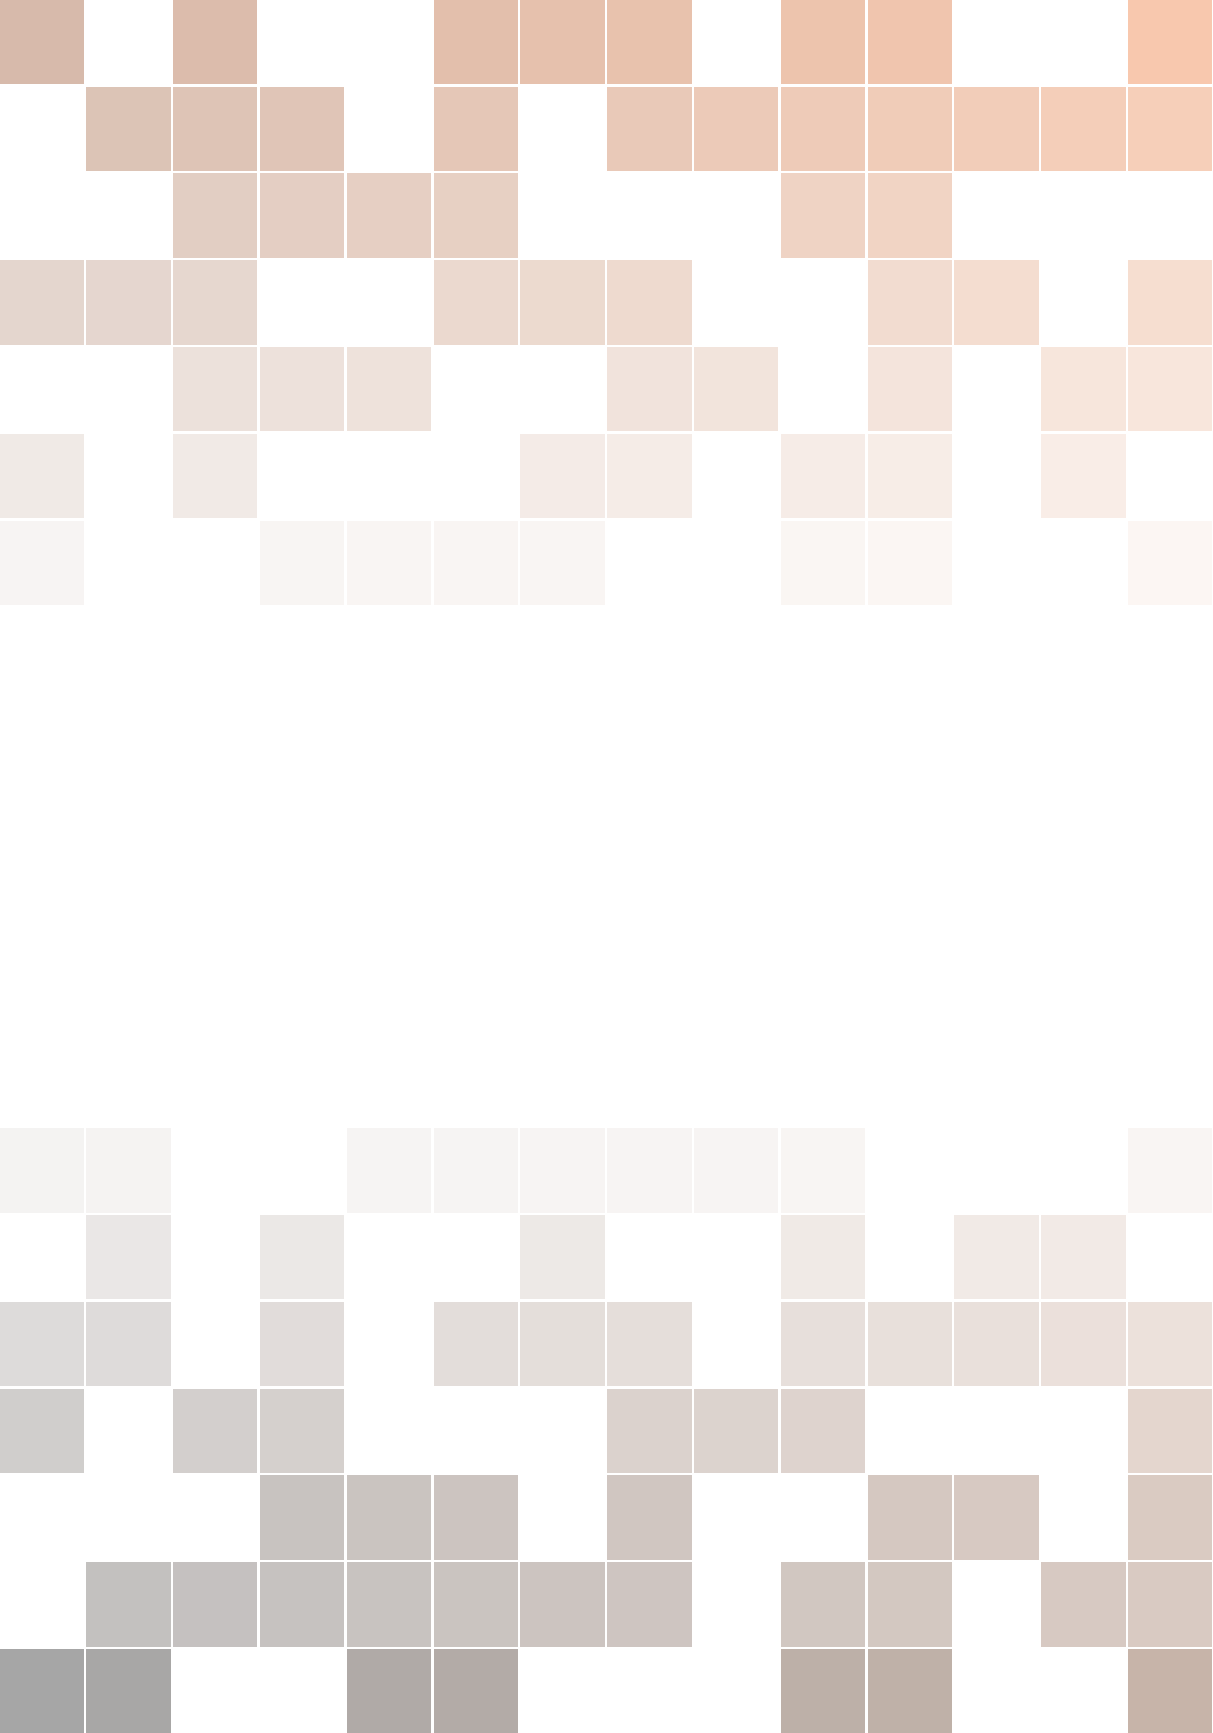
\includegraphics[width=\paperwidth]{background}};
\draw (current page.center) node [fill=ocre!30!white,fill opacity=0.6,text opacity=1,inner sep=1cm]{\Huge\centering\bfseries\sffamily\parbox[c][][t]{\paperwidth}{\centering Álgebra Linear\\[15pt] % Book title
{\Large Notas de Aula 2/2018}\\[20pt] % Subtitle
{\huge Jos\'e Ant\^onio O. Freitas}\\
{\large \today}}}; % Author name

\end{tikzpicture}
\vfill
\endgroup

%----------------------------------------------------------------------------------------
%   COPYRIGHT PAGE
%----------------------------------------------------------------------------------------

\newpage
~\vfill
\thispagestyle{empty}

\noindent \ccbyncsa\ Este texto est\'a licenciado sob uma \textbf{Licen\c{c}a Creative Commons Atribui\c{c}\~ao-N\~aoComercial-CompartilhaIgual 3.0 Brasil} \href{http://creativecommons.org/licenses/by-nc-sa/3.0/br/deed.pt\_BR}{\textit{http://creativecommons.org/licenses/by-nc-sa/3.0/br/deed.pt\_BR}}\\ % Copyright notice

%----------------------------------------------------------------------------------------
%   TABLE OF CONTENTS
%----------------------------------------------------------------------------------------

\usechapterimagefalse % If you don't want to include a chapter image, use this to toggle images off - it can be enabled later with \usechapterimagetrue

\chapterimage{chapter_head_1.pdf} % Table of contents heading image

\pagestyle{empty} % No headers

\tableofcontents % Print the table of contents itself

\cleardoublepage % Forces the first chapter to start on an odd page so it's on the right

\pagestyle{fancy} % Print headers again


%!TEX program = xelatex
%!TEX root = Algebra_Linear.tex
%%Usar makeindex -s indexstyle.ist arquivo no terminal para gerar o {\'\i}ndice remissivo agrupado por inicial
%%Ap\'os executar pdflatex arquivo
\chapter{Sistemas Lineares E Matrizes}

%\section{Preliminares}

\section{Corpos}\label{ssub:corpos}

\begin{definicao}\index{Corpos}
Um conjunto n\~ao vazio $\cp{K}$ \'e chamado de \textbf{corpo} se em $\cp{K}$ podemos definir duas opera\c{c}\~oes, denotadas por
$\oplus$ (adi\c{c}\~ao) e $\otimes$ (multiplica\c{c}\~ao) de modo que
\begin{align*}
a \oplus b \in \cp{K}\\
a \otimes b \in \cp{K}
\end{align*}
para todos $a$, $b \in \cp{K}$ e que satisfa\c{c}am as seguintes propriedades:
\begin{itemize}

	\item[A1)] \textbf{Comutatividade da adi\c{c}\~ao}: $a \oplus b = b \oplus a$ para todos $a$, $b \in \cp{K}$;
	\item[A2)] \textbf{Associatividade da adi\c{c}\~ao}: $a \oplus (b \oplus c) = (a \oplus b) \oplus c$, para todos $a$, $b$ e $c \in \cp{K}$;
	\item[A3)] \textbf{Elemento neutro da adi\c{c}\~ao}: Existe um elemento em $\cp{K}$, denotado por $0_\cp{K}$ ou simplesmente $0$ e chamado de \textbf{elemento neutro da adi\c{c}\~ao}, que satisfaz
	\[
		a \oplus 0_\cp{K} = a = 0_\cp{K} \oplus a
	\]
	para todo $a \in \cp{K}$. (Elemento neutro da adi\c{c}\~ao)
	\item[A4)] \textbf{Elemento oposto da adi\c{c}\~ao}: Para cada $a \in \cp{K}$, existe um elemento em $\cp{K}$, denotado por $-a$ e chamado de \textbf{oposto} de $a$ ou \textbf{inverso aditivo} de $a$ tal que
	\[
		a \oplus (-a) = 0_\cp{K} = (-a) \oplus a.
	\]
	\item[M1)] \textbf{Comutatividade da multiplica\c{c}\~ao}: $a \otimes b = b \otimes a$ para todos $a$, $b \in \cp{K}$;
	\item[M2)] \textbf{Associatividade da multiplica\c{c}\~ao}: $a \otimes (b \otimes c) = (a \otimes b) \otimes c$, para todos $a$, $b$ e $c \in \cp{K}$;
	\item[M3)] \textbf{Elemento neutro da multiplica\c{c}\~ao}: Existe um elemento em $\cp{K}$, denotado por $1_\cp{K}$ ou simplesmente $1$ e chamado de \textbf{elemento neutro da multiplica\c{c}\~ao} ou \textbf{unidade}, que satisfaz
	\[
		a \otimes 1_\cp{K} = a = 1_\cp{K} \otimes a
	\]
	para todo $a \in \cp{K}$.
	\item[M4)] \textbf{Elemento inverso da multiplica\c{c}\~ao}: Para cada $a \in \cp{K}$, $a \ne 0_{\cp{K}}$, existe um elemento em $\cp{K}$, denotado por $a^{-1}$ e chamado de \textbf{inverso multiplicativo} de $a$ 
	tal que
	\[
		a \otimes a^{-1} = 1_\cp{K} = a^{-1} \otimes a.
	\]
	\item[D)] \textbf{Distributividade da soma em rela\c{c}\~ao \`a multiplica\c{c}\~ao}: $(a \oplus b)\otimes c = a\otimes c \oplus b\otimes c$, para todos $a$, $b$ e $c \in \cp{K}$.
\end{itemize}
\end{definicao}

Para simplificar a nota\c{c}\~ao vamos escrever
\[
a \otimes b = ab.
\]
Denotamos um corpo $\cp{K}$ pela terna $(\cp{K}, \otimes, \oplus)$. Quando n\~ao houver chance de confus\~ao em rela\c{c}\~ao \`as opera\c{c}\~oes de soma e multiplica\c{c}\~ao envolvidas no corpo $(\cp{K}, \otimes, \oplus)$, vamos simplesmente dizer que $\cp{K}$ \'e um corpo. Os elementos de um corpo $\cp{K}$ s\~ao chamados de \textbf{escalares}.

\begin{exemplo}
\begin{enumerate}[label={\arabic*})]
	\item S\~ao exemplos de corpos os conjuntos: $\rac$, $\real$, $\complex$ com as opera\c{c}\~oes de soma e multiplica\c{c}\~oes usuais destes conjuntos.

	\item O conjunto $\z$ com a soma e multiplica\c{c}\~oes usuais n\~ao \'e um corpo, pois por exemplo, n\~ao existe $b \in \z$ tal que $2b = 1$.

	\item Seja
	\[
	\rac{[\sqrt{2}]} = \{a + b\sqrt{2} \mid a,\ b \in \rac\}.
	\]
	Dados $a + b\sqrt{2}$, $c + d\sqrt{2} \in \rac{[\sqrt{2}]}$, defina
	\begin{align*}
	(a + b\sqrt{2}) + (c + d\sqrt{2}) = (a + c) + (b + d)\sqrt{2}\\
	(a + b\sqrt{2})(c + d\sqrt{2}) = (ac + 2bd) + (ad + bc)\sqrt{2}
	\end{align*}
	Al\'em disso, $a + b\sqrt{2} = c + d\sqrt{2}$ se, e somente se, $a = c$ e $b = d$.
	Aqui o elemento neutro da adi\c{c}\~ao \'e $0$, o elemento neutro da multiplica\c{c}\~ao \'e $1$, o oposto aditivo de $a + b\sqrt{2}$ \'e $-a - b\sqrt{2}$ e o inverso multiplicativo de $a + b\sqrt{2}$ \'e $\dfrac{a - b\sqrt{2}}{a^2 - 2b^2}$ para $a \ne 0$ ou $b \ne 0$.

	\item Considere as opera\c{c}\~oes $\oplus$ e $\otimes$ em $\rac$ definidas por
	\begin{align*}
		x \oplus y = x + y - 3\\
		x \otimes y = x + y - \dfrac{xy}{3},
	\end{align*}
	para todos $x$, $y \in \rac$. Ent\~ao $(\rac, \oplus, \otimes)$ \'e um corpo.
	\begin{solucao}
		De fato, para todos $x$, $y$ e $z \in \rac$ temos:
		\begin{enumerate}[label={\arabic*})]
			\item $x \oplus y = x + y - 3 = y + x - 3 = y \oplus x$.
			Logo $x \oplus y = y \oplus x$.

			\item Temos
			\begin{align*}
				(x \oplus y) \oplus z &= (x + y - 3) \oplus z = (x + y - 3) + z - 3 = x + y + z - 6\\
				x \oplus ( y \oplus z) &= x \oplus (y + z - 3) = x + (y + z - 3) - 3 = x + y + z - 6.
			\end{align*} Logo $(x \oplus y) \oplus z = x \oplus ( y \oplus z)$, como quer{\'\i}amos.

			\item Tome $0_{\cp{K}} = 3$. Ent\~ao para todo $x \in \rac$ temos
			\[
				x \oplus 0_{\cp{K}} = x \oplus 3 = x + 3 - x = x.
			\]
			Logo $0_{\cp{K}} = 3$ \'e o elemento neutro da opera\c{c}\~ao $\oplus$ em $\rac$.

			\item Para $x \in \rac$ tome $y = 6 - x \in \rac$. Assim
			\[
				x \oplus y = x \oplus (6 - x) = x + (6 - x ) - 3 = 3 = 0_{\cp{K}},
			\]
			logo $y = 6 - x$ \'e o oposto de $x$ na adi\c{c}\~ao $\oplus$ definida em $\rac$.

			\item $x \otimes y = x + y - \dfrac{xy}{3} = y + x - \dfrac{yx}{3} = y \otimes x$, para todos $x$, $y \in \rac$.

			\item Para $x$, $y$ e $z \in \rac$ temos
			\begin{align*}
				(x \otimes y) \otimes z &= \left(x + y - \dfrac{xy}{3}\right) \otimes z = \left(x + y - \dfrac{xy}{3}\right) + y - \dfrac{\left(x + y - \dfrac{xy}{3}\right)z}{3} \\ &= x + y - \dfrac{xy}{3} + z - \dfrac{xz}{3} - \dfrac{yz}{3} + \dfrac{xyz}{9}\\
				x \otimes (y \otimes z) &= x \otimes \left(y + z - \dfrac{yz}{3}\right) = x + \left(y + z - \dfrac{yz}{3}\right) - \dfrac{x\left(y + z - \dfrac{yz}{3}\right)}{3} \\ &= x + y + z - \dfrac{yz}{3} - \dfrac{xy}{3} - \dfrac{xz}{3} + \dfrac{xyz}{9},
			\end{align*}
			logo $(x \otimes y) \otimes z = x \otimes (y \otimes z)$, como quer{\'\i}amos.

			\item Tome $1_{\cp{K}} = 0$. Ent\~ao
			\[
				x \otimes 1_{\cp{K}} = x \otimes 0 = x + 0 - \dfrac{x0}{3} = x,
			\]
			para todo $x \in \rac$. Logo $1_{\cp{K}} = 0$ \'e a unidade da opera\c{c}\~ao $\otimes$ em $\rac$.

			\item Dado $x \in \rac$, $x \ne 3 = 0_{\cp{K}}$ tome $y = \dfrac{-3x}{3 - x} \in \rac$. Temos
			\[
				x \otimes y = x \otimes \dfrac{-3x}{3 - x} = x + \dfrac{-3x}{3 - x} - \dfrac{x\left(\dfrac{-3x}{3 - x}\right)}{3} = 0 = 1_{\cp{K}}.
			\]
			Logo $y = \dfrac{-3x}{3 - x}$ \'e o inverso multiplicativo de $x$ na opera\c{c}\~ao $\otimes$ em $\rac$.

			\item Para todos $x$, $y$ e $z \in \rac$ temos
			\begin{align*}
				(x \oplus y) \otimes z &= (x + y - 3) \otimes z = (x + y - 3) + z - \dfrac{(x + y - 3)z}{3} \\ &= x + y - 3 + z - \dfrac{xz}{3} - \dfrac{yz}{3} + z\\
				(x \otimes z) \oplus (y \otimes z) &= \left(x + z - \dfrac{xz}{3}\right) \oplus \left(y + z - \dfrac{yz}{3}\right) \\ &= x + z - \dfrac{xz}{3} + y + z - \dfrac{yz}{3} - 3,
			\end{align*}
			Logo $(x \oplus y) \otimes z = (x \otimes z) \oplus (y \otimes z)$.
		\end{enumerate}
		Portanto $(\rac, \oplus, \otimes)$ \'e um corpo.
	\end{solucao}
\end{enumerate}
\end{exemplo}

\begin{proposicao}
	Seja $(\cp{K}, +, \cdot)$ um corpo. Ent\~ao:
	\begin{enumerate}[label={\roman*})]
		\item O elemento neutro da soma \'e \'unico.
		\item O oposto aditivo de cada elemento de $\cp{K}$ \'e \'unico.
		\item Vale a lei do cancelamento, isto \'e, se $a + b = a + c$ ent\~ao $b = c$.
		\item Para todo $a \in \cp{K}$, $a\cdot 0_\cp{K} = 0_\cp{K}$.
		\item O elemento neutro da multiplica\c{c}\~ao \'e \'unico.
		\item O inverso de um elemento n\~ao nulo \'e \'unico.
		\item Se $a \in \cp{K}$ \'e tal que $a \ne 0_\cp{K}$ e $ab = ac$, ent\~ao $b = c$.
		\item Se $ab = 0_\cp{K}$, com $a$ e $b \in \cp{K}$, ent\~ao $a = 0_\cp{K}$ ou $b = 0_\cp{K}$.
	\end{enumerate}
\end{proposicao}
\begin{prova}
	Vamos provar algumas propriedades.
	\begin{enumerate}[label={\roman*})]
		\item De fato, suponha que $0_1$ e $0_2$ sejam elementos neutros da soma em $\cp{K}$. Temos
		\[
			0_1 = 0_1 + 0_2 = 0_2.
		\]
	
		\item Sejam $b$ e $c$ elementos opostos de $a$. Daí
		\begin{align*}
			a + b &= 0_\cp{K}\\
			a + c &= 0_\cp{K}.
		\end{align*}
	 	Ent\~ao
		\[
			b = b + 0_\cp{K} = b + (c + a) = (b + a) + c = 0_\cp{K} + c = c.
		\]
		
		\item Temos
		\begin{align*}
			b &= b + 0_{\cp{K}} = b + (a + (-a)) = (b + a) + (-a) \\ &= (a + b) + (-a) = (a + c) + (-a) = (c + a) + (-a) \\ &= c + (a + (-a)) = c + 0_{\cp{K}} \\ &= c
		\end{align*}
		como queríamos.
	
		\item De fato,
		\[
			a\cdot 0_\cp{K} + 0_\cp{K} = a\cdot 0_\cp{K} = a\cdot (0_\cp{K} + 0_\cp{K}) = a\cdot 0_\cp{K} + a\cdot 0_\cp{K},
		\]
		logo pela lei do cancelamento, $a\cdot 0_\cp{K} = 0_\cp{K}$ como quer{\'\i}amos.
	
	
		\item
		De fato, suponha que $1_a$ e $1_b$ sejam elementos neutros da multiplica\c{c}\~ao. Ent\~ao
		\[
			1_a = 1_a\cdot 1_b = 1_b.
		\]
	
		\item Dado $a \in \cp{K}$, $a \ne 0_{\cp{K}}$, suponha que $b$, $c \in \cp{K}$ sejam tais que
		\[
			ab = 1_{\cp{K}} \quad ac = 1_{\cp{K}}.
		\]
		Ent\~ao
		\[
			b = 1_{\cp{K}}b = (ac)b = c(ab) = c1_{\cp{K}} = c.
		\]
		
		\item De fato,
		\begin{align*}
			b &= b1_{\cp{K}} = b(aa^{-1}) = (ba)a^{-1} = (ab)a^{-1} \\ &= (ac)a^{-1} = (ca)a^{-1} = c(aa^{-1}) = c1_{\cp{K}} \\ &= c
		\end{align*}
	
		\item
		Suponha que $a \ne 0_\cp{K}$, ent\~ao existe $a^{-1}$. Da{\'\i}
		\begin{align*}
			&ab = 0_\cp{K}\\
			&a^{-1}(ab) = a^{-1}0_\cp{K}\\
			&1b = 0_\cp{K}\\
			&b = 0_\cp{K}.
		\end{align*}
	\end{enumerate}
\end{prova}


% \begin{observacao}
% Os elementos de um corpo qualquer $\cp{K}$ s\~ao chamados de \textbf{escalares}.
% \end{observacao}

\section{Corpos Finitos}\label{sec:corpor_finitos}\index{Corpos!Finitos}

Seja $p \in \z$ um n\'umero primo. Dado $a \in \z$, sempre \'e poss{\'\i}vel escrever
\[
	a = bp + r,
\]
onde $b$, $r \in \z$ e $0 \le r \le p - 1$. Assim quando efetuamos a divis\~ao inteira de qualquer n\'umero inteiro $a$ por $p$ os poss{\'\i}veis restos s\~ao: $0$, 
$1$, $2$, \dots, $p -1 $.

Assim vamos considerar o seguinte conjunto
\[
	\z_p = \{\overline{0}, \overline{1}, \overline{2}, \dots, \overline{p - 1}\}
\]
onde
\begin{align*}
	&\overline{0} = \{bp \mid b \in \z\} = \{0, \pm p, \pm 2p, \pm 3p, \dots\}\\
	&\overline{1} = \{bp + 1\mid b \in \z\} = \{\pm p + 1, \pm 2p + 1, \pm 3p + 1, \dots\}\\
	&\overline{2} = \{bp + 2\mid b \in \z\} = \{\pm p + 2, \pm 2p + 2, \pm 3p + 2, \dots\}\\
	\vdots\\
	&\overline{p - 1} = \{bp + (p - 1) \mid b \in \z\} = \{(b + 1)p - 1) \mid b \in \z\}\\ &= \{cp - 1 \mid c \in \z\} = \{-1, \pm p - 1, \pm 2p - 1, \pm 3p - 1, \dots\}.
\end{align*}

defina em $\z_p$ a soma $\oplus$ e a multiplica\c{c}\~ao $\otimes$ por: para $\overline{x}$, $\overline{y} \in \z_p$
\begin{align*}
	\overline{x} \oplus \overline{y} = \overline{x + y}\\
	\overline{x} \otimes \overline{y} = \overline{xy},
\end{align*}
onde sob a barra estamos usando a soma e multiplica\c{c}\~ao usuais dos inteiros. Para determinar o valor de $\overline{x + y}$ e de $\overline{xy}$, encontramos o resto da divis\~ao inteira de $x + y$ por $p$ e de $xy$ por $p$. Logo
\begin{align*}
	\overline{x} \oplus \overline{y} \in \z_p\\
	\overline{x} \otimes \overline{y} \in \z_p.
\end{align*}

\begin{exemplos}
\begin{enumerate}[label={\arabic*})]
	\item Para $p = 3$ os poss{\'\i}veis restos na divis\~ao inteira s\~ao: $0$, $1$ e $2$. Da{\'\i}
		\[
			\z_3 = \{\overline{0}, \overline{1}, \overline{2}\}
		\]
	e temos
	\begin{center}
		\begin{tabular}{|c|c|c|c|c|c|}
			\hline
			$\oplus$ &\rule{0pt}{2.5ex} $\overline{0}$ & $\overline{1}$ & $\overline{2}$\\\hline
			$\rule{0pt}{2.5ex}\overline{0}$ & $\overline{0}$ & $\overline{1}$ & $\overline{2}$\\\hline
			$\rule{0pt}{2.5ex}\overline{1}$ & $\overline{1}$ & $\overline{2}$ & $\overline{0}$\\\hline
			$\rule{0pt}{2.5ex}\overline{2}$ & $\overline{2}$ & $\overline{0}$ & $\overline{1}$\\\hline
			\end{tabular} \qquad \begin{tabular}{|c|c|c|c|c|c|}
			\hline
			$\otimes$ &\rule{0pt}{2.5ex} $\overline{0}$ & $\overline{1}$ & $\overline{2}$\\\hline
			$\rule{0pt}{2.5ex}\overline{0}$ & $\overline{0}$ & $\overline{0}$ & $\overline{0}$\\\hline
			$\rule{0pt}{2.5ex}\overline{1}$ & $\overline{0}$ & $\overline{1}$ & $\overline{2}$\\\hline
			$\rule{0pt}{2.5ex}\overline{2}$ & $\overline{0}$ & $\overline{2}$ & $\overline{1}$\\\hline
		\end{tabular}
	\end{center}
	Note que a soma $\oplus$ e o produto $\otimes$ em $\z_3$ s\~ao comutativos, a soma possui elemento neutro que \'e $\overline{0}$, todo elemento possui
	oposto aditivo. A multiplica\c{c}\~ao possui unidade que \'e $\overline{1}$ e todo elemento n\~ao nulo possui inverso multiplicativo. \'E simples verificar que a soma e o produto em $\z_3$ s\~ao associativos e o produto \'e distributivo em rela\c{c}\~ao \`a soma. Portanto, $(\z_3, \oplus, \otimes)$ \'e um corpo. Al\'em disso, em tal corpo temos
	\[
		(\overline{1} \oplus \overline{1}) \oplus \overline{1} = (\overline{1 + 1}) \oplus \overline{1} = \overline{2} \oplus \overline{1} = \overline{3} = \overline{0}.
	\]
	e $\overline{1} \ne \overline{0}$.

	\item Para $p = 5$ os poss{\'\i}veis restos na divis\~ao inteira s\~ao: $0$, $1$, $2$, $3$ e $4$. Da{\'\i}
		\[
			\z_5 = \{\overline{0}, \overline{1}, \overline{2}, \overline{3}, \overline{4}\}
		\]
	e temos
		\begin{center}
			\begin{tabular}{|c|c|c|c|c|c|c|c|}
				\hline
				$\oplus$ &\rule{0pt}{2.5ex}$\overline{0}$ & $\overline{1}$ & $\overline{2}$ & $\overline{3}$ & $\overline{4}$\\\hline
				$\rule{0pt}{2.5ex}\overline{0}$ & $\overline{0}$ & $\overline{1}$ & $\overline{2}$ & $\overline{3}$ & $\overline{4}$\\\hline
				$\rule{0pt}{2.5ex}\overline{1}$ & $\overline{1}$ & $\overline{2}$ & $\overline{3}$ & $\overline{4}$ & $\overline{0}$\\\hline
				$\rule{0pt}{2.5ex}\overline{2}$ & $\overline{2}$ & $\overline{3}$ & $\overline{4}$& $\overline{0}$ & $\overline{1}$ \\\hline
				$\rule{0pt}{2.5ex}\overline{3}$ & $\overline{3}$ & $\overline{4}$ & $\overline{0}$& $\overline{1}$ & $\overline{2}$ \\\hline
				$\rule{0pt}{2.5ex}\overline{4}$ & $\overline{4}$ & $\overline{0}$ & $\overline{1}$& $\overline{2}$ & $\overline{3}$ \\\hline
			\end{tabular} \qquad 
			\begin{tabular}{|c|c|c|c|c|c|}
				\hline
				$\otimes$ &\rule{0pt}{2.5ex} $\overline{0}$ & $\overline{1}$ & $\overline{2}$ & $\overline{3}$ & $\overline{4}$\\\hline
				$\rule{0pt}{2.5ex}\overline{0}$ & $\overline{0}$ & $\overline{0}$ & $\overline{0}$ & $\overline{0}$ & $\overline{0}$\\\hline
				$\rule{0pt}{2.5ex}\overline{1}$ & $\overline{0}$ & $\overline{1}$ & $\overline{2}$ & $\overline{3}$ & $\overline{4}$\\\hline
				$\rule{0pt}{2.5ex}\overline{2}$ & $\overline{0}$ & $\overline{2}$ & $\overline{4}$& $\overline{1}$ & $\overline{3}$ \\\hline
				$\rule{0pt}{2.5ex}\overline{3}$ & $\overline{0}$ & $\overline{3}$ & $\overline{1}$& $\overline{4}$ & $\overline{2}$ \\\hline
				$\rule{0pt}{2.5ex}\overline{4}$ & $\overline{0}$ & $\overline{4}$ & $\overline{3}$& $\overline{2}$ & $\overline{1}$ \\\hline
			\end{tabular}
		\end{center}
	Note que a soma $\oplus$ e o produto $\otimes$ em $\z_5$ s\~ao comutativos, a soma possui elemento neutro que \'e $\overline{0}$, todo elemento possui
	oposto aditivo. A multiplica\c{c}\~ao possui unidade que \'e $\overline{1}$ e todo elemento n\~ao nulo possui inverso multiplicativo. \'E simples verificar que a soma e o produto em $\z_5$ s\~ao associativos e o produto \'e distributivo em rela\c{c}\~ao \`a soma. Portanto, $(\z_5, \oplus, \otimes)$ \'e um corpo. Al\'em disso, em tal corpo temos
	\[
		\overline{1} \oplus \overline{1} \oplus \overline{1} \oplus \overline{1} \oplus \overline{1} = \overline{1 + 1 + 1 + 1 + 1} = \overline{5} = \overline{0}.
	\]
	e $\overline{1} \ne \overline{0}$.
\end{enumerate}
\end{exemplos}

\begin{teorema}
Para todo $p \in \z$, $p$ n\'umero primo, $(\z_p, \oplus, \otimes)$ \'e um corpo.
\end{teorema}
\begin{prova}
Dados $\overline{x}$, $\overline{y}$, $\overline{z} \in \z_p$ temos:
\begin{enumerate}
	\item[A1)] $\overline{x} \oplus \overline{y} = \overline{x + y} = \overline{y + x} = \overline{y} \oplus \overline{x}$;
	\item[A2)] $(\overline{x} \oplus \overline{y}) \oplus \overline{z} = (\overline{x + y}) \oplus \overline{z} = \overline{(x + y) + z} = \overline{x + (y + z)} = \overline{x} \oplus (\overline{y} \oplus \overline{z}) = \overline{x} \oplus (\overline{y} \oplus \overline{z})$
	\item[A3)] Temos que $\overline{0} \in \z_p$ e para todo $\overline{x} \in \z_p$:
	\[
	\overline{0} \oplus \overline{x} = \overline{x} \oplus \overline{0} = \overline{x + 0} = \overline{x}.
	\]
	Logo $\overline{0}$ \'e o elemento neutro da adi\c{c}\~ao em $\z_p$.
	\item[A4)] Dado $\overline{x} \in \z_p$, tome $\overline{p - x} \in \z_p$, pois $0 \le p - x \le p - 1$. Assim
	\[
	\overline{x} \oplus \overline{p - x} = \overline{p - x} \oplus \overline{x} = \overline{(p - x) + x} = \overline{p} = \overline{0}.
	\]
	Logo todo elemento de $\z_p$ possui oposto aditivo.
	\item[M1)] $\overline{x} \otimes \overline{y} = \overline{x\cdot y} = \overline{y \cdot x} = \overline{y} \otimes \overline{x}$.
	\item[M2)] $(\overline{x} \otimes \overline{y}) \otimes \overline{z} = (\overline{x\cdot y}) \otimes \overline{z} = \overline{(x\cdot y) \cdot z} = 
	\overline{x\cdot (y\cdot z)} = \overline{x} \otimes (\overline{y} \otimes \overline{z})$.
	\item[M3)] O elemento $\overline{1} \in \z_p$ \'e tal que
	\[
	\overline{1} \otimes \overline{x} = \overline{x} \otimes \overline{1} = \overline{x\cdot 1} = \overline{x}
	\]
	para todo $\overline{x} \in \z_p$.
	\item[M4)] Primeiramente, como $p$ \'e um n\'umero primo ent\~ao existem $y$, $z \in \z$ tais que
	\[
	xy + pz = 1
	\]
	para todo $x \in \{1, 2, \dots, p - 1\}$. Logo,
	\begin{align*}
	&\overline{xy + pz} = \overline{1}\\
	&\overline{xy} \oplus \overline{pz} = \overline{1}\\
	&\overline{x} \otimes \overline{y} + \overline{p} \otimes \overline{z} = \overline{1}\\
	&\overline{x} \otimes \overline{y} = \overline{1}
	\end{align*}
	uma vez que $\overline{p} = \overline{0}$. Como $\overline{y}$ \'e obtido pelo resto da divis\~ao inteira de $y$ por $p$, ent\~ao 
	$\overline{y} \in \z_p$. Observe que $y \ne 0$ pois $p \ge 2$ e $y \ne p$ pois sen\~ao $(x + z)p = 1$ o que \'e imposs{\'\i}vel uma vez que $p \ge 2$. Logo $\overline{y} \ne \overline{0}$ e assim todo elemento $\overline{x} \in \z_p$ possui inverso multiplicativo.
	\item[D)] $(\overline{x} \oplus \overline{y}) \otimes \overline{z}= (\overline{x + y}) \otimes \overline{z} = \overline{(x + y) \cdot z} = \overline{xz + yz} = \overline{xz} \oplus \overline{yz} = \overline{x} \otimes \overline{z} \oplus \overline{y} \otimes \overline{z}$.
\end{enumerate}
Portanto, $(\z_p, \oplus, \otimes)$ \'e um corpo, como quer{\'\i}amos demonstrar.
\end{prova}

\begin{observacao}
\begin{enumerate}
	\item Se $p$ n\~ao for um n\'umero primo, $(\z_p, \oplus, \otimes)$ pode n\~ao ser corpo. Por exemplo, em $\z_6$ temos $\overline{2} \ne \overline{0}$ e $\overline{3} \ne \overline{0}$, mas
	\[
	\overline{2}\otimes \overline{3} = \overline{2\cdot 3} = \overline{6} = \overline{0}.
	\]

	\item Para simplificar a nota\c{c}\~ao vamos denotar $\oplus$ por $+$ e $\otimes$ por $\cdot$. Assim vamos dizer simplesmente que $(\z_p, +, \cdot)$ \'e um corpo.
\end{enumerate}
\end{observacao}


\section{Sistemas Lineares}\label{ssub:sistemas_lineares}
Seja $\cp{K}$ um corpo. Consideremos o problema de determinar $n$ escalares, ou seja, $n$ elementos $x_1$, $x_2$, \dots, $x_n$ em $\cp{K}$ que satisfa\c{c}am simultaneamente as equa\c{c}\~oes
\begin{equation}\label{sistemalinear}\index{Sistema Linear}
\begin{cases}
a_{11}x_1 + a_{12}x_2 + \cdots + a_{1n}x_n = b_1\\
a_{21}x_1 + a_{22}x_2 + \cdots + a_{2n}x_n = b_2\\
\qquad \vdots\\
a_{m1}x_1 + a_{m2}x_2 + \cdots + a_{mn}x_n = b_m\\
\end{cases}
\end{equation}
onde $b_1$, \dots, $b_m$ e $a_{ij}$, $1 \le i \le m$, $1 \le j \le n$ s\~ao elementos de $\cp{K}$ previamente conhecidos. Chamamos \eqref{sistemalinear} de um \textbf{sistema de $m$ equa\c{c}\~oes lineares a $n$ inc\'ognitas} $x_1$, $x_2$, \dots, $x_n$. Toda $n$-upla $(\alpha_1, \alpha_2, \dots, \alpha_n)$ onde $\alpha_i \in \cp{K}$ para $1 \le i \le n$, que satisfazem a cada uma das equa\c{c}\~oes de \eqref{sistemalinear} \'e chamada de uma \textbf{solu\c{c}\~ao} do sistema. 

Se $b_1 = b_2 = \cdots = b_m = 0_\cp{K} \in K$, dizemos que o sistema
\begin{equation}\label{sistemalinearhomogeneo}\index{Sistema Linear}
\begin{cases}
a_{11}x_1 + a_{12}x_2 + \cdots + a_{1n}x_n = 0_\cp{K}\\
a_{21}x_1 + a_{22}x_2 + \cdots + a_{2n}x_n = 0_\cp{K}\\
\qquad \vdots\\
a_{m1}x_1 + a_{m2}x_2 + \cdots + a_{mn}x_n = 0_\cp{K}\\
\end{cases}
\end{equation}
\'e um \textbf{sistema linear homog\^eneo}, ou que cada uma de suas equa\c{c}\~oes \'e homog\^enea. Observe que tal sistema sempre possui solu\c{c}\~ao, a saber, $x_1 = x_2 = \cdots = x_n = 0_\cp{K}$.

O m\'etodo mais importante para determinar as solu\c{c}\~oes de um sistema de equa\c{c}\~oes lineares \'e o m\'etodo do \textbf{escalonamento}. Por exemplo, considere o sistema
\begin{equation}\label{exemploplo1}
\begin{cases}
2x_1 - x_2 + x_3 = 0\\
x_1 + 3x_2 + 4x_ 3 = 0
\end{cases}
\end{equation}
onde o corpo considerado \'e $\real$.

Observe que multiplicando a segunda equa\c{c}\~ao de \eqref{exemploplo1} por $-2$ e somando o resultado \`a primeira equa\c{c}\~ao obtemos
\[
-7x_2 - 7x_3 = 0
\]
o que resulta em $x_2 = -x_3$. Agora se multiplicarmos a primeira equa\c{c}\~ao de \eqref{exemploplo1} por $3$ e somarmos com a segunda, obtemos
\[
7x_1 + 7x_3 = 0
\]
e da{\'\i} $x_1 = -x_3$.

Assim para que uma terna $(x_1, x_2, x_3)$ de n\'umeros reais seja solu\c{c}\~ao de \eqref{exemploplo1} deve satisfazer
\[
x_1 = x_2 = -x_3.
\]
Por outro lado, qualquer terna da forma $(a, a, -a)$ \'e solu\c{c}\~ao de \eqref{exemploplo1}. Portanto a solu\c{c}\~ao de \eqref{exemploplo1} \'e da forma
\[
(a, a, -a)
\]
onde $a \in \real$.

No caso de um sistema linear da forma \eqref{sistemalinear}, o processo de elemina\c{c}\~ao de vari\'aveis ser\'a feito mediante o uso de 3 tipos de opera\c{c}\~oes. S\~ao elas:
\begin{itemize}
	\item[$e_1$)] Troca da posi\c{c}\~ao de duas equa\c{c}\~oes.
	\item[$e_2$)] Multiplica\c{c}\~ao de uma equa\c{c}\~ao por um escalar n\~ao nulo.
	\item[$e_3$)] Substitui\c{c}\~ao de uma equa\c{c}\~ao pela soma desta equa\c{c}\~ao com alguma outra.
\end{itemize}

Estas tr\^es opera\c{c}\~oes s\~ao chamadas de \textbf{opera\c{c}\~oes elementares}.\index{Opera\c{c}\~oes Elementares}

\begin{exemplo}
Considere o seguinte sistema sobre o corpo $\real$:
\[
\begin{cases}
x_1 + 4x_2 + 3x_3 = 1\\
2x_1 + 5x_2 + 4x_3 = 4\\
x_1 - 3x_2 - 2x_3 = 5
\end{cases}
\]
Efetuando opera\c{c}\~oes elementares podemos escrever:
\begin{align*}
&\begin{cases}
x_1 + 4x_2 + 3x_3 = 1\\
2x_1 + 5x_2 + 4x_3 = 4 & L_2 \rightarrow L_2 - 2L_1\\
x_1 - 3x_2 - 2x_3 = 5
\end{cases} \sim
\begin{cases}
x_1 + 4x_2 + 3x_3 = 1\\
\phantom{0x_1} -3x_2 - 2x_3 = 2\\
x_1 - 3x_2 - 2x_3 = 5 & L_3 \rightarrow L_2 - L_1
\end{cases}\\ & \sim
\begin{cases}
x_1 + 4x_2 + 3x_3 = 1\\
\phantom{0x_1} - 3x_2 - 2x_3 = 2 & L_2 \rightarrow (-1/3)L_2\\
\phantom{0x_1} - 7x_2 - 5x_3 = 4
\end{cases} \sim
\begin{cases}
x_1 + 4x_2 + 3x_3 = 1\\
\phantom{0x_1} x_2 + (2/3)x_3 = (-2/3)\\
\phantom{0x_1} - 7x_2 - 5x_3 = 4 & L_3 \rightarrow L_3 + 7L_2
\end{cases}\\ & \sim
\begin{cases}
x_1 + 4x_2 + 3x_3 = 1\\
\phantom{0x_1} x_2 + (2/3)x_3 = (-2/3)\\
\phantom{0x_1} \phantom{0x_2}  -(1/3)x_3 = -(2/3)
\end{cases}
\end{align*}
Assim encontramos
\[
x_1 = 3, \quad x_2 = -2, \quad x_3 = 2.
\]
\end{exemplo}

\begin{definicao}\index{Sistemas Equivalentes}
Dois sistemas de equa\c{c}\~oes lineares s\~ao chamados de \textbf{equivalentes} se, e somente, se toda solu\c{c}\~ao de qualquer um dos sistemas \'e solu\c{c}\~ao do outro.
\end{definicao}

Dado um sistema linear
\begin{equation}
\begin{cases}
a_{11}x_1 + a_{12}x_2 + \cdots + a_{1n}x_n = b_1\\
a_{21}x_1 + a_{22}x_2 + \cdots + a_{2n}x_n = b_2\\
\qquad \vdots\\
a_{m1}x_1 + a_{m2}x_2 + \cdots + a_{mn}x_n = b_m\\
\end{cases}
\end{equation}
com o objetivo de simplificar sua nota\c{c}\~ao vamos escrev\^e-lo na forma
\begin{equation}\label{formamatricial}
AX = B
\end{equation}
onde
\begin{enumerate}
	\item
	\[
	A = \begin{bmatrix}
	a_{11} & a_{12} & \cdots & a_{1n}\\
	\vdots & & & \vdots\\
	a_{m1} & a_{m2} & \cdots & a_{mn}
	\end{bmatrix}_{m\times n}; \quad a_{ij} \in \cp{K},\ 1 \le i \le m,\ 1 \le j \le n
	\]
	\'e chamada \textbf{matriz dos coeficientes do sistema};
	\item
	\[
	X = \begin{bmatrix}
	x_1\\
	x_2\\
	\vdots\\
	x_n
	\end{bmatrix}_{n \times 1}
	\]
	\item
	\[
	B = \begin{bmatrix}
	b_1\\
	b_2\\
	\vdots\\
	b_m
	\end{bmatrix}_{m \times 1}; \quad b_1, b_2, \dots, b_m \in \cp{K}.
	\]
\end{enumerate}

Uma outra matriz que podemos associar ao sistema \eqref{sistemalinear} \'e
\[
\begin{amatrix}{4}
a_{11} & a_{12} & \cdots & a_{1n} & b_1\\
a_{21} & a_{22} & \cdots & a_{2n} & b_2\\
\vdots & \vdots & \vdots & \vdots & \vdots\\
a_{m1} & a_{m2} & \cdots & a_{mn} & b_m\\
\end{amatrix}
\]
que \'e chamada de \textbf{matriz ampliada do sistema} ou \textbf{matriz aumentada do sistema}.

Na forma matricial as opera\c{c}\~oes elementares s\~ao descritas como:\index{Opera\c{c}\~oes Elementares!Sobre Matrizes}
\begin{itemize}
	\item[$e_1$)] Trocar a $i$-\'esima linha de $A$ pela $j$-\'esima linha de $A$: $L_i \leftrightarrow L_j$;
	\item[$e_2$)] Multiplica\c{c}\~ao da $i$-\'esima linha de $A$ por um escalar $\alpha \in \cp{K}$ n\~ao nulo: $L_i \rightarrow \alpha L_i$;
	\item[$e_3$)] Substitui\c{c}\~ao da $i$-\'esima linha de $A$ pela $i$-\'esima linha mais $\alpha$ vezes a $j$-\'esima linha: $L_i \rightarrow L_i + \alpha L_j$.
\end{itemize}

\begin{observacao}
Denotaremos a matriz
\[
\begin{bmatrix}
0_{\cp{K}} & 0_{\cp{K}} \cdots & 0_{\cp{K}}\\
0_{\cp{K}} & 0_{\cp{K}} \cdots & 0_{\cp{K}}\\
\vdots & & \vdots\\
0_{\cp{K}} & 0_{\cp{K}} \cdots & 0_{\cp{K}}
\end{bmatrix},
\]
onde $0_{\cp{K}}$ \'e o elemento neutro da soma no corpo $\cp{K}$, simplesmente por $0$.
\end{observacao}

Uma raz\~ao para nos restringirmos a estes tr\^es tipos simples de opera\c{c}\~oes sobre linhas \'e que, tendo efetuado uma tal opera\c{c}\~ao $e$ sobre uma matriz $A$, podemos desfazer essa opera\c{c}\~ao efetuando uma opera\c{c}\~ao de mesmo tipo sobre $e(A)$.

\begin{teorema}
A cada opera\c{c}\~ao elementar sobre linhas $e$, corresponde uma opera\c{c}\~ao elementar sobre linhas $e'$, do mesmo tipo que $e$, tal que $e'(e(A)) = A$ para qualquer matriz $A$. Em outras palavras, a opera\c{c}\~ao inversa de uma opera\c{c}\~ao elementar sobre linhas existe e \'e uma opera\c{c}\~ao elementar sobre linhas do mesmo tipo.
\end{teorema}
\begin{prova}
Vamos verificar que cada uma das opera\c{c}\~oes elementares possui uma opera\c{c}\~ao inversa. Seja $A$ uma matriz $m \times n$ sobre o corpo $\cp{K}$
\[
A = \begin{bmatrix}
a_{11} & a_{12} & \cdots & a_{1n}\\
a_{21} & a_{22} & \cdots & a_{2n}\\
\vdots & & & \vdots\\
a_{m1} & a_{m2} & \cdots & a_{mn}
\end{bmatrix}.
\]
\begin{enumerate}
	\item [e1)] Suponha que $e$ seja a opera\c{c}\~ao que troca a linha $i$ pela linha $j$ de $A$. Temos
	\[
	e(A) = 
	\begin{bmatrix}
	a_{11} & a_{12} & \cdots & a_{1n}\\
	a_{21} & a_{22} & \cdots & a_{2n}\\
	\vdots\\
	a_{j1} & a_{j2} & \cdots & a_{jn}\\
	\vdots\\
	a_{i1} & a_{i2} & \cdots & a_{in}\\
	\vdots\\
	a_{m1} & a_{m2} & \cdots & a_{mn}
	\end{bmatrix}.
	\]
	Ent\~ao, seja $e'$ a opera\c{c}\~ao que troca a linha $i$ pela linha $j$ de $e(A)$. Assim
	\[
	e'(e(A)) = A
	\]
	como quer{\'\i}amos.

	\item [e2)] Suponha que $e$ seja a opera\c{c}\~ao que multiplica a $i$-\'esima de $A$ por $\alpha \in \cp{K}$, onde $\alpha \ne 0_\cp{K}$. Temos
	\[
	e(A) = 
	\begin{bmatrix}
	a_{11} & a_{12} & \cdots & a_{1n}\\
	a_{21} & a_{22} & \cdots & a_{2n}\\
	\vdots\\
	\alpha a_{i1} & \alpha a_{i2} & \cdots & \alpha a_{in}\\
	\vdots\\
	a_{m1} & a_{m2} & \cdots & a_{mn}
	\end{bmatrix}.
	\]
	Seja $e'$ a opera\c{c}\~ao que multiplica a linha $i$ de $e(A)$ por $\alpha^{-1} \in \cp{K}$. Ent\~ao
	\[
	e'(e(A)) = A.
	\]
	\item [e3)] Suponha que $e$ seja a opera\c{c}\~ao que substitui a linha $i$ de $A$ pela linha $i$ mais $\alpha$ vezes a linha $j$. Temos
	\[
	e(A) = 
	\begin{bmatrix}
	a_{11} & a_{12} & \cdots & a_{1n}\\
	a_{21} & a_{22} & \cdots & a_{2n}\\
	\vdots\\
	a_{i1} + \alpha a_{j1} & a_{i2} + \alpha a_{j2} & \cdots & a_{in} + \alpha a_{jn}\\
	\vdots\\
	a_{m1} & a_{m2} & \cdots & a_{mn}
	\end{bmatrix}.
	\]
	Seja $e'$ a opera\c{c}\~ao que substitui a linha $i$ de $e(A)$ pela linha $i$ mais $(-\alpha)$ vezes a linha $j$. Ent\~ao
	\[
	e'(e(A)) = 
	\begin{bmatrix}
	a_{11} & a_{12} & \cdots & a_{1n}\\
	a_{21} & a_{22} & \cdots & a_{2n}\\
	\vdots\\
	a_{i1} + \alpha a_{j1} + (-\alpha)a_{j1} & a_{i2} + \alpha a_{j2} + (-\alpha)a_{j2} & \cdots & a_{in} + \alpha a_{jn} + (-\alpha)a_{jn}\\
	\vdots\\
	a_{m1} & a_{m2} & \cdots & a_{mn}
	\end{bmatrix}.
	\]
	e assim
	\[
	e'(e(A)) = A.
	\]
\end{enumerate}
Portanto cada opera\c{c}\~ao elementar sobre linhas possui uma opera\c{c}\~ao inversa.
\end{prova}

\begin{definicao}\index{Matriz!Linha Equivalente}
Se $A$ e $B$ s\~ao matrizes $m \times n$, dizemos que $B$ \'e \textbf{linha-equivalente} a $A$, se $B$ for obtida de $A$ atrav\'es de uma quantidade finita de opera\c{c}\~oes elementares sobre as linhas de $A$.
\end{definicao}

\begin{notacao}
$A \rightarrow B$ ou $A \sim B$.
\end{notacao}

\begin{exemplo}
A matriz
\[
B = \begin{bmatrix}
1 & 0\\
0 & 1\\
0 & 0
\end{bmatrix}
\]
\'e linha equivalente \`a matriz
\[
A = \begin{bmatrix}
\phantom{-}1 & \phantom{-}0\\
\phantom{-}4 & -1\\
-3 & \phantom{-}4
\end{bmatrix}
\]
pois
		\begin{align*}
			A &= \begin{gmatrix}[b]
			\phantom{-}1 & \phantom{-}0\\
			\phantom{-}4 & -1\\
			-3 & \phantom{-}4
			\rowops
			\add[-4]{0}{1}
			\end{gmatrix}\leadsto\begin{gmatrix}[b]
			\phantom{-}1 & \phantom{-}0\\
			\phantom{-}0 & -1\\
			-3 & \phantom{-}4
			\rowops
			\add[3]{0}{2}
			\end{gmatrix}\leadsto\begin{gmatrix}[b]
			1 & \phantom{-}0\\
			0 & -1\\
			0 & \phantom{-}4
			\rowops
			\mult1{\times -1}
			\end{gmatrix}\\&\leadsto\begin{gmatrix}[b]
			1 & 0\\
			0 & 1\\
			0 & 4
			\rowops
			\add[-4]{1}{2}
			\end{gmatrix}\leadsto\begin{bmatrix}
			1 & 0\\
			0 & 1\\
			0 & 0
			\end{bmatrix} = B.
		\end{align*}
\end{exemplo}

\begin{teorema}
Se $X_1$ e $X_2$ s\~ao duas solu\c{c}\~oes de
\[
AX = 0,
\]
ent\~ao $\alpha X_1 + \beta X_2$ tamb\'em \'e solu\c{c}\~ao de $AX = 0$, para quaisquer $\alpha$, $\beta \in \cp{K}$.
\end{teorema}

\begin{teorema}
Se $A$ e $B$ s\~ao matrizes $m \times n$ que s\~ao linha-equivalentes, ent\~ao os sistemas homog\^eneos de equa\c{c}\~oes lineares $AX = 0$ e $BX = 0$ t\^em exatamente as mesmas solu\c{c}\~oes.
\end{teorema}
\begin{prova}
Suponha que podemos obter a matriz $B$ \`a partir da matriz $A$ por meio de uma sequ\^encia finita de opera\c{c}\~oes elementares sobre linhas:
\[
A = A_0 \sim A_1 \sim A_2 \sim \cdots \sim A_r = B.
\]
Nesta situa\c{c}\~ao, para provar que $AX = 0$ e $BX = 0$ tem as mesmas solu\c{c}\~oes basta provar que $A_iX = 0$ e $A_{i + 1}X = 0$ tem as mesmas solu\c{c}\~oes, isto \'e, que uma opera\c{c}\~ao elementar sobre linhas n\~ao altera o conjunto das solu\c{c}\~oes.

Assim podemos supor que $B$ \'e obtida de $A$ por meio de uma \'unica opera\c{c}\~ao elementar. Qualquer que seja a opera\c{c}\~ao elementar, $e_1$ ou $e_2$ ou $e_3$, cada equa\c{c}\~ao do sistema $BX = 0$ ser\'a uma combina\c{c}\~ao das equa\c{c}\~oes do sistema $AX = 0$. Como a inversa de uma opera\c{c}\~ao elementar sobre linhas \'e ainda uma opera\c{c}\~ao elementar sobre linhas, cada equa\c{c}\~ao de $AX = 0$ tamb\'em ser\'a uma combina\c{c}\~ao das equa\c{c}\~oes em $BX = 0$. Logo toda solu\c{c}\~ao de $AX = 0$ tamb\'em \'e solu\c{c}\~ao de $BX = 0$ e toda solu\c{c}\~ao de $BX = 0$ tamb\'em \'e solu\c{c}\~ao de $AX = 0$, como quer{\'\i}amos.
\end{prova}

\begin{exemplo}
Considere o sistema homog\^eneo $AX = 0$, onde:
\begin{enumerate}[label={\arabic*})]
	\item $A = \begin{bmatrix}
	2 & -1 & \phantom{-}3 & \phantom{-}2\\
	1 & \phantom{-}4 & \phantom{-}0 & -1\\
	2 & \phantom{-}6 & -1 & \phantom{-}5
	\end{bmatrix}.$
	Para encontrar a solu\c{c}\~ao deste sistema s\'o precisamos encontrar uma matriz $B$ que seja linha equivalente \`a $A$ e que seja mais f\'acil de determinar a solu\c{c}\~ao do sistema resultante. Assim, vamos executar as opera\c{c}\~oes elementares em $A$ de modo a simplific\'a-la:
	\begin{align*}
	A = \begin{gmatrix}[b]
	2 & -1 & \phantom{-}3 & \phantom{-}2\\
	1 & \phantom{-}4 & \phantom{-}0 & -1\\
	2 & \phantom{-}6 & -1 & \phantom{-}5
	\rowops
	\swap01
	\end{gmatrix}\leadsto\begin{gmatrix}[b]
	1 & \phantom{-}4 & \phantom{-}0 & -1\\
	2 & -1 & \phantom{-}3 & \phantom{-}2\\
	2 & \phantom{-}6 & -1 & \phantom{-}5
	\rowops
	\add[-2]{0}{1}
	\add[-2]{0}{2}
	\end{gmatrix}\\\leadsto\begin{gmatrix}[b]
	1 & \phantom{-}4 & \phantom{-}0 & -1\\
	0 & -9 & \phantom{-}3 & \phantom{-}4\\
	0 & -2 & -1 & \phantom{-}7
	\rowops
	\swap12
	\end{gmatrix}\leadsto\begin{gmatrix}[b]
	1 & \phantom{-}4 & 0 & -1\\
	0 & -2 & -1 & \phantom{-}7\\
	0 & -9 & \phantom{-}3 & \phantom{-}4
	\rowops
	\mult1{\times -1/2}
	\end{gmatrix}\\\leadsto\begin{gmatrix}[b]
	1 & \phantom{-}4 & 0 & -1\\
	0 & \phantom{-}1 & 1/2 & -7/2\\
	0 & -9 & 3 & \phantom{-}4
	\rowops
	\add[9]{1}{2}
	\end{gmatrix}\leadsto\begin{bmatrix}
	1 & 4 & 0 & -1\\
	0 & 1 & 1/2 & -7/2\\
	0 & 0 & 15/2 & -55/2
	\end{bmatrix}
	\end{align*}
	assim obtemos o sistema
	\[
	\begin{cases}
	x_1 + 4x_2 - x_4 = 0\\
	x_2 + (1/2)x_3 - (7/2)x_4 = 0\\
	(15/2)/x_3 - (55/2)x_4 = 0
	\end{cases}.
	\]
	Isolando $x_3$ na \'ultima equa\c{c}\~ao temos a solu\c{c}\~ao dada por
	\[
	S = \left\{\left(\dfrac{-17}{3}x_4, \dfrac{5}{3}x_4, \dfrac{11}{3}x_4, x_4\right) \mid x_4 \in \real\right\}.
	\]

	\item $A = \begin{bmatrix}
	-1 & i\\
	-i & 1\\
	\phantom{-}1 & 2
	\end{bmatrix}.$ Temos:
	\begin{align*}
	A &= \begin{gmatrix}[b]
	-1 & i\\
	-i & 1\\
	\phantom{-}1 & 2
	\rowops
	\swap02
	\end{gmatrix}\leadsto\begin{gmatrix}[b]
	\phantom{-}1 & 2\\
	-i & 1\\
	-1 & i
	\rowops
	\add[i]{0}{1}
	\add{0}{2}
	\end{gmatrix}\\&\leadsto\begin{gmatrix}[b]
	1 & 2\\
	0 & 1 + 2i\\
	0 & 2 + i
	\rowops
	\mult1{\times \dfrac{1 - 2i}{5}}
	\end{gmatrix}\leadsto\begin{gmatrix}[b]
	1 & 2\\
	0 & 1\\
	0 & 2 + i
	\rowops
	\add[-(2 + i)]{1}{2}
	\end{gmatrix}\\&\leadsto\begin{bmatrix}
	1 & 2\\
	0 & 1\\
	0 & 0
	\end{bmatrix}.
	\end{align*}
	Assim obtemos o sistema
	\[
	\begin{cases}
	x_1 + 2x_2 = 0\\
	x_2 = 0
	\end{cases}
	\]
	cuja solu\c{c}\~ao \'e $x_1 = x_2 = 0$.
\end{enumerate}
\end{exemplo}

\begin{definicao}\label{linhareduzida}\index{Matriz!Linha-reduzida}
Uma matriz R $m \times n$ \'e chamada de \textbf{linha-reduzida} se:
\begin{enumerate}[label={\roman*})]
\item o primeiro elemento n\~ao nulo em cada linha n\~ao nula de $R$ \'e $1_\cp{K}$.
\item cada coluna de $R$ que cont\'em o primeiro elemento n\~ao nulo de alguma linha tem todos os seus outros elementos nulos.
\end{enumerate}
\end{definicao}

\begin{exemplo}
\begin{enumerate}[label={\arabic*})]
	\item Um exemplo de uma matriz linha-reduzida \'e a matriz identidade $n \times n$. Tal matriz pode ser definida por
	\[
	I = (a_{ij})_{1 \le i,j \le n}
	\]
	onde
	\[
	a_{ij} = \delta_{ij} = \begin{cases}
	1, & \mbox{ se } i = j\\
	0, & \mbox{ se } i \ne j 
	\end{cases}.
	\]
	O s{\'\i}mbolo $\delta_{ij}$ \'e chamada \textbf{s{\'\i}mbolo de Kronecher} \'e ser\'a utilizado com certa frequ\^encia.
	\item As matrizes
	\[
	A = \begin{bmatrix}
	1 & 0 & \phantom{-}0 & 0\\
	0 & 1 & -1 & 0\\
	0 & 0 & \phantom{-}1 & 0
	\end{bmatrix}; \quad B = \begin{bmatrix}
	0 & 2 & \phantom{-}1\\
	1 & 0 & -3\\
	0 & 0 & \phantom{-}0
	\end{bmatrix}
	\]
	n\~ao s\~ao linha-reduzidas.
\end{enumerate}
\end{exemplo}

\begin{teorema}
Toda matriz $m \times n$ sobre um corpo $\cp{K}$ \'e linha-equivalente a uma matriz linha-reduzida.
\end{teorema}
\begin{prova}
Seja $A$ uma matriz $m \times n$ sobre um corpo $\cp{K}$. Se todo elemento na primeira linha de $A$ \'e $0_\cp{K}$, ent\~ao a condi\c{c}\~ao (a) de \eqref{linhareduzida} est\'a satisfeita no que diz respeito a linha 1. Se a linha 1 tem um elemento n\~ao nulo, seja $r$ o menor inteiro positivo $j$ tal que $a_{1r} \ne 0$. Multiplique a linha 1 por $a_{1r}^{-1}$ e condi\c{c}\~ao (a) de \eqref{linhareduzida} est\'a satisfeita em rela\c{c}\~ao a linha 1. Agora, para cada $i \ge 2$, somemos $-a_{ir}$ vezes a linha 1 \`a linha i. Assim o primeiro elemento n\~ao nulo da linha 1 ocorre na coluna $r$, este elemento \'e $1_\cp{K}$, e todos os outros elementos da coluna $r$ s\~ao nulos.

Considere agora a matriz que resultou das opera\c{c}\~oes acima. Se todo elemento na linha 2 \'e nulo, nada h\'a a fazer. Se algum elemento na linha 2 \'e n\~ao nulo, multiplicamos a linha 2 por um escalar de modo que o primeiro elemento n\~ao nulo da linha 2 seja $1_\cp{K}$. Caso o primeiro elemento n\~ao nulo da linha 1 ocorra na coluna $r$, o primeiro elemento n\~ao nulo da linha 2 n\~ao pode ocorrer na coluna $r$. Digamos ent\~ao que ele ocorra na coluna $r'$. Somando m\'ultiplos adequados da linha 2 \`as diversas linhas, podemos fazer com que todos os elementos da coluna $r'$ seja nulos, com exce\c{c}\~ao do elemento $1_\cp{K}$ da linha 2. O importante a ser observado \'e: ao efetuarmos estas \'ultimas opera\c{c}\~oes, n\~ao alteramos os elementos da linha 1 na colunas 1, 2, \dots, $r$; al\'em disso, n\~ao alteramos nenhum elemento da coluna $r$. \'E claro que, se a linha 1 fosse identicamente nula, as opera\c{c}\~oes com a linha 2 n\~ao afetariam a linha 1.

Operando com uma linha de cada vez da maneira acima, \'e evidente que, com uma quantidade finita de passos, chegamos a uma matriz linha-reduzida.
\end{prova}

\begin{definicao}\index{Matriz!Na forma escada}
Uma matriz $R$ $m \times n$ \'e chamada uma \textbf{matriz linha-reduzida \`a forma em escada} se:
\begin{enumerate}[label={\roman*})]
	\item $R$ \'e linha-reduzida;
	\item toda linha de $R$ cujos elementos s\~ao todos nulos ocorre abaixo de todas as linhas que possuem um elemento n\~ao-nulo;
	\item se as linhas 1, 2, \dots, $r$ s\~ao as linhas n\~ao-nulas de $R$ e se o primeiro elemento n\~ao-nulo da linha $i$ ocorre na coluna $k_i$, $i = 1$, \dots, $r$, ent\~ao $k_1 < k_2 < \cdots < k_r$.
\end{enumerate}
\end{definicao}

\begin{exemplo}
\begin{enumerate}[label={\arabic*})]
	\item  A matriz identidade e a matriz nula s\~ao linha-reduzidas \`a forma escada;
	\item $\begin{bmatrix}
	1 & 0 & \phantom{-}0 & 0\\
	0 & 1 & -1 & 0\\
	0 & 0 & \phantom{-}1 & 0
	\end{bmatrix}$ N\~ao \'e linha-reduzida \`a forma escada.
	\item $\begin{bmatrix}
	0 & 2 & \phantom{-}1\\
	1 & 0 & -3\\
	0 & 0 & \phantom{-}0
	\end{bmatrix}$ N\~ao \'e linha-reduzida \`a forma escada.
	\item $\begin{bmatrix}
	0 & 1 & -3 & 0 & 2\\
	0 & 0 & \phantom{-}0 & 1 & 2\\
	0 & 0 & \phantom{-}0 & 0 & 0
	\end{bmatrix}$ \'E linha-reduzida \`a forma escada.
\end{enumerate}
\end{exemplo}

\begin{teorema}
Toda matriz $A$ $m \times n$ \'e linha-equivalente a uma matriz linha-reduzida \`a forma em escada.
\end{teorema}
\begin{prova}
Sabemos que $A$ \'e linha-equivalente a uma matriz linha-reduzida. Portanto, basta notar que, efetuando uma quantidade finita de permuta\c{c}\~oes das linhas de uma matriz linha-reduzida, podemos transform\'a-la numa matriz linha-reduzida \`a forma em escada.
\end{prova}

\begin{definicao}\index{Posto!de uma matriz}\index{Nulidade!de uma matriz}
Dada uma matriz $A$ $m \times n$, seja $B$ a matriz $m \times n$ linha-reduzida \`a forma em escada linha-equivalente a $A$. O \textbf{posto} de $A$, denotado por $p$, \'e o n\'umero de linhas n\~ao-nulas de $B$. A \textbf{nulidade} de $A$ \'e o n\'umero $n - p$.
\end{definicao}

\begin{exemplo}
Qual o posto e a nulidade da matriz $A$, onde
\[
A = \begin{bmatrix}
\phantom{-}1 & \phantom{-}2 & 1 & 0\\
-1 & \phantom{-}0 & 3 & 5\\
\phantom{-}1 & -2 & 1 & 1
\end{bmatrix}?
\]
Precisamos primeiro reduzir $A$ a sua forma escada:
\begin{align*}
A &= \begin{gmatrix}[b]
\phantom{-}1 & \phantom{-}2 & 1 & 0\\
-1 & \phantom{-}0 & 3 & 5\\
\phantom{-}1 & -2 & 1 & 1
\rowops
\add{0}{1}
\add[-1]{0}{2}
\end{gmatrix}\leadsto\begin{gmatrix}[b]
1 & \phantom{-}2 & 1 & 0\\
0 & \phantom{-}2 & 4 & 5\\
0 & -4 & 0 & 1
\rowops
\mult1{\times (1/2)}
\end{gmatrix}\\&\leadsto\begin{gmatrix}[b]
1 & \phantom{-}2 & 1 & 0\\
0 & \phantom{-}1 & 2 & 5/2\\
0 & -4 & 0 & 1
\rowops
\add[-2]{1}{0}
\add[4]{1}{2}
\end{gmatrix}\leadsto\begin{gmatrix}[b]
1 & 0 & -3 & -5\\
0 & 1 & \phantom{-}2 & \phantom{-}5/2\\
0 & 0 & \phantom{-}8 & \phantom{-}11
\rowops
\mult2{\times 1/8}
\end{gmatrix}\\&\leadsto\begin{gmatrix}[b]
1 & 0 & -3 & -5\\
0 & 1 & \phantom{-}2 & \phantom{-}5/2\\
0 & 0 & \phantom{-}1 & \phantom{-}11/8
\rowops
\add[3]{2}{0}
\add[-2]{2}{1}
\end{gmatrix}\\&\leadsto\begin{bmatrix}
1 & 0 & 0 & -7/8\\
0 & 1 & 0 & -1/4\\
0 & 0 & 1 & \phantom{-}11/8
\end{bmatrix}
\end{align*}
Logo o posto de $A$ \'e $p = 3$ e a nulidade \'e $n - p = 4 - 3 = 1$.
\end{exemplo}

Considere o sistema
\begin{equation}\label{equacaolinear}
AX = B
\end{equation}
onde $A$ \'e uma matriz $m \times n$ e $B$ \'e uma matriz $m \times 1$, ambas com entradas no corpo $\cp{K}$ e $X$ \'e uma matriz $n \times 1$. Observe que, enquanto uma sistema homog\^eneo $AX = 0$ sempre admite a solu\c{c}\~ao
\[
x_1 = x_2 = \cdots = x_n = 0_\cp{K},
\]
um sistema n\~ao homog\^eneo pode ter:
\begin{enumerate}
	\item Uma \'unica solu\c{c}\~ao $x_1 = \alpha_1$, $x_2 = \alpha_2$, \dots, $x_n = \alpha_n$, onde $\alpha_i \in \cp{K}$, para $i = 1$, 2, \dots, $n$. Neste caso dizemos que o sistema \'e \textbf{poss{\'\i}vel e determinado}.
	\item Mais de uma solu\c{c}\~ao. Neste caso dizemos que o sistema \'e \textbf{poss{\'\i}vel e indeterminado}. Caso o corpo $\cp{K}$ tenha infinitos elementos, o sistema ter\'a infinitas solu\c{c}\~oes.
	\item Nenhuma solu\c{c}\~ao. Neste caso dizemos o que sistema \'e \textbf{imposs{\'\i}vel}.
\end{enumerate}

Com o objetivo de resolver o sistema \eqref{equacaolinear} vamos come\c{c}ar formando a matriz ampliada
\[
P = [A|B] = \begin{amatrix}{4}
a_{11} & a_{12} & \dots & a_{1n} & b_1\\
a_{21} & a_{22} & \dots & a_{2n} & b_2\\
\vdots & \vdots & \vdots & \vdots & \vdots\\
a_{m1} & a_{m2} & \dots & a_{mn} & b_m\\
\end{amatrix}_{m \times (n + 1)}.
\]

Sabemos que $P$ \'e linha-equivalente a uma matriz linha-reduzida \`a forma em escada $R$. A \'ultima coluna de $R$ cont\'em elementos $z_1$, $z_2$, \dots, $z_m$ que s\~ao resultados das opera\c{c}\~oes elementares aplicadas \`a matriz $P$. Seja 
\[
Z = \begin{bmatrix}
z_1\\
z_2\\
\vdots\\
z_m
\end{bmatrix}.
\]
Ent\~ao $R$ pode ser escrita como $R = [R' \mid Z]$. Como no caso homog\^eneo, \'e poss{\'\i}vel mostrar que os sistemas
\[
AX = B \mbox{ e } R'X = Z
\]
possuem exatamente as mesmas solu\c{c}\~oes.

As possibilidades para as solu\c{c}\~oes de tal sistema s\~ao descritas no seguinte teorema:

\begin{teorema}
Considere o sistema
\[
AX = B
\]
onde $A$ \'e uma matriz $m \times n$ e $B$ \'e uma matriz $m \times 1$, ambas com entradas no corpo $\cp{K}$ e $X$ \'e uma matriz $n \times 1$. Ent\~ao:
\begin{enumerate}[label={\roman*})]
	\item O sistema tem solu\c{c}\~ao se, e somente se, o posto da matriz ampliada \'e igual ao posto da matriz dos coeficientes.

	\item Se a matriz ampliada e a matriz dos coeficientes t\^em o mesmo posto $p$ e $p = n$, ent\~ao a solu\c{c}\~ao \'e \'unica.

	\item Se a matriz ampliada e a matriz dos coeficientes t\^em o mesmo posto $p$ e $p < n$, ent\~ao podemos escolher $n - p$ vari\'aveis, e as outras $p$ vari\'aveis ser\~ao dadas em fun\c{c}\~ao destas $n - p$ vari\'aveis escolhidas.
\end{enumerate}
O n\'umero $n - p$ \'e chamado de \textbf{grau de liberdade} e as $n - p$ vari\'aveis s\~ao chamadas de \textbf{vari\'aveis livres}.
\end{teorema}
\begin{prova}
\textit{$1^a$ Parte: Se existe solu\c{c}\~ao para o sistema, ent\~ao a matriz ampliada e a matriz dos coeficientes t\^em o mesmo posto:} Para mostrar isso, vamos provar que se a matriz ampliada e a matriz dos coeficientes tiverem postos diferentes, ent\~ao o sistema n\~ao ter\'a solu\c{c}\~ao. Observe primeiro que o posto da matriz ampliada n\~ao pode ser menor que o posto da matriz dos coeficientes uma vez que a matriz ampliada \'e formada a partir da matriz dos coeficientes. Assim o \'unico caso poss{\'\i}vel \'e o posto da matriz ampliada ser maior que o posto da matriz dos coeficientes. Ent\~ao esta matriz, quando reduzida \`a forma em escada deve conter uma linha da forma
\[
\begin{bmatrix}
0_\cp{K} & 0_\cp{K} & \cdots & 0_\cp{K} & \mid & 1_\cp{K}
\end{bmatrix}.
\]
Logo o sistema associado a essa matriz tem uma equa\c{c}\~ao do tipo
\[
0_\cp{K}x_1 + 0_\cp{K}x_2 + \cdots + 0_\cp{K}x_n = 1_\cp{K}
\]
o que \'e imposs{\'\i}vel. Logo n\~ao existe solu\c{c}\~ao.

\textit{$2^a$ Parte: Se o posto \'e igual, ent\~ao existe solu\c{c}\~ao:} Nesta situa\c{c}\~ao podem ocorrer dois casos:
\begin{enumerate}
	\item Se $p = n$, ent\~ao a matriz linha-reduzida \`a forma em escada tem a forma
	\[
	\begin{amatrix}{5}
	1_\cp{K} & 0_\cp{K} & 0_\cp{K} & \cdots & 0_\cp{K} & z_1\\
	0_\cp{K} & 1_\cp{K} & 0_\cp{K} & \cdots & 0_\cp{K} & z_2\\
	\vdots & \vdots & \vdots & \vdots & \vdots & \vdots\\
	0_\cp{K} & 0_\cp{K} & 0_\cp{K} & \cdots & 1_\cp{K} & z_n\\
	0_\cp{K} & 0_\cp{K} & 0_\cp{K} & 0_\cp{K} & 0_\cp{K} & 0_\cp{K}\\
	\vdots & \vdots & \vdots & \vdots & \vdots & \vdots\\
	0_\cp{K} & 0_\cp{K} & 0_\cp{K} & 0_\cp{K} & 0_\cp{K} & 0_\cp{K}
	\end{amatrix}
	\]
	e a solu\c{c}\~ao do sistema ser\'a
	\[
	x_1 = z_1, x_2 = z_2, \cdots, x_n = z_n.
	\]
	\item Se $p \ne n$, ent\~ao devemos ter $p < n$. Caso $p > n$, como a matriz est\'a na forma escada o elemento $1_\cp{K}$ deve ocorrer em duas linhas diferentes, mas na mesma coluna. Mas neste caso, podemos anular uma destas linhas repetidas. Logo, $p < n$. Neste caso a matriz na forma escada pode ter a forma:
	\begin{enumerate}
		\item \[
		\begin{amatrix}{9}
		1_\cp{K} & 0_\cp{K} & 0_\cp{K} & \cdots & 0_\cp{K} & a_{1p+1} & a_{1p+2} & \cdots & a_{1n} & z_1\\
		0_\cp{K} & 1_\cp{K} & 0_\cp{K} & \cdots & 0_\cp{K} & a_{2p+1} & a_{2p+2} & \cdots & a_{2n} & z_2\\
		\vdots & \vdots & \vdots & \vdots & \vdots & \vdots & \vdots & \vdots & \vdots & \vdots\\
		0_\cp{K} & 0_\cp{K} & 0_\cp{K} & \cdots & 1_\cp{K} & a_{pp+1} & a_{pp+2} & \cdots & a_{pn} & z_p\\
		0_\cp{K} & 0_\cp{K} & 0_\cp{K} & 0_\cp{K} & 0_\cp{K} & 0_\cp{K} & 0_\cp{K} & \cdots & 0_\cp{K} & 0_\cp{K}\\
		\vdots & \vdots & \vdots & \vdots & \vdots & \vdots & \vdots & \vdots & \vdots & \vdots\\
		0_\cp{K} & 0_\cp{K} & 0_\cp{K} & 0_\cp{K} & 0_\cp{K} & 0_\cp{K} & 0_\cp{K} & \cdots & 0_\cp{K}  & 0_\cp{K}
		\end{amatrix}.
		\]
		Neste caso teremos
		\[
		\begin{cases}
		x_1 = z_1 + (-a_{1 p + 1})x_{p + 1} + (-a_{1 p + 2})x_{p + 2} + \cdots + (-a_{1n})x_{n}\\
		x_2 = z_2 + (-a_{2 p + 1})x_{p + 1} + (-a_{2 p + 2})x_{p + 2} + \cdots + (-a_{2n})x_{n}\\
		\qquad \vdots\\
		x_p = z_p + (-a_{p p + 1})x_{p + 1} + (-a_{p p + 2})x_{p + 2} + \cdots + (-a_{pn})x_{n}\\
		\end{cases}
		\]
		e o sistema ter\'a mais de uma solu\c{c}\~ao, sendo $x_{p + 1}$ , $x_{p + 2}$, \dots, $x_n$ as vari\'aveis livres.
		\item Uma segunda forma a ser considerada para a matriz reduzida \'e
		\[
		\begin{amatrix}{9}
		0_\cp{K} & 1_\cp{K} & 0_\cp{K} & \cdots & 0_\cp{K} & a_{1p+2} & a_{1p+3} & \cdots & a_{1n} & z_1\\
		0_\cp{K} & 0_\cp{K} & 1_\cp{K} & \cdots & 0_\cp{K} & a_{2p+2} & a_{2p+3} & \cdots & a_{2n} & z_2\\
		\vdots & \vdots & \vdots & \vdots & \vdots & \vdots & \vdots & \vdots & \vdots & \vdots\\
		0_\cp{K} & 0_\cp{K} & 0_\cp{K} & \cdots & 1_\cp{K} & a_{pp+2} & a_{pp+3} & \cdots & a_{pn} & z_p\\
		0_\cp{K} & 0_\cp{K} & 0_\cp{K} & 0_\cp{K} & 0_\cp{K} & 0_\cp{K} & 0_\cp{K} & \cdots & 0_\cp{K} & 0_\cp{K}\\
		\vdots & \vdots & \vdots & \vdots & \vdots & \vdots & \vdots & \vdots & \vdots & \vdots\\
		0_\cp{K} & 0_\cp{K} & 0_\cp{K} & 0_\cp{K} & 0_\cp{K} & 0_\cp{K} & 0_\cp{K} & \cdots & 0_\cp{K}  & 0_\cp{K}
		\end{amatrix}.
		\]
		Neste caso teremos
		\[
		\begin{cases}
		x_2 = z_1 + (-a_{1 p + 2})x_{p + 2} + (-a_{1 p + 3})x_{p + 3} + \cdots + (-a_{1n})x_{n}\\
		x_3 = z_2 + (-a_{2 p + 3})x_{p + 3} + (-a_{2 p + 3})x_{p + 3} + \cdots + (-a_{2n})x_{n}\\
		\qquad \vdots\\
		x_{p+1} = z_p + (-a_{p p + 2})x_{p + 2} + (-a_{p p + 3})x_{p + 3} + \cdots + (-a_{pn})x_{n}\\
		\end{cases}
		\]
		e o sistema ter\'a mais de uma solu\c{c}\~ao, sendo $x_1$, $x_{p + 1}$ , $x_{p + 2}$, \dots, $x_n$ as vari\'aveis livres.
	\end{enumerate}
	Prosseguindo com esse racioc{\'\i}nio, vemos que para qualquer posto $p < n$ teremos um sistema com mais de uma solu\c{c}\~ao e $n - p$ vari\'aveis livres.
\end{enumerate}
Portanto a condi\c{c}\~ao (i) do teorema est\'a provada.

Observe que os itens (ii) e (iii) foram automaticamente demonstrados nos itens (a) e (b) anteriores.

Logo o teorema est\'a provado.
\end{prova}

\begin{exemplo}
Encontre a solu\c{c}\~ao dos seguintes sistemas lineares:
\begin{enumerate}[label={\arabic*})]
	\item $\begin{cases}
	x + 3y + z = 0\\
	2x + 6y + 2z = 0\\
	-x - 3y - z = 0
	\end{cases}$ em $\real$.
	\begin{solucao}
	A matriz dos coeficentes deste sistema \'e
	\[
	\begin{bmatrix}
	\phantom{-}1 & \phantom{-}3 & 1\\
	\phantom{-}2 & \phantom{-}6 & 2\\
	-1 & -3 & -1
	\end{bmatrix}.
	\]
	Aplicando as opera\c{c}\~oes elementares para reduzir $A$ \`a forma em escada:
	\begin{align*}
	A = \begin{gmatrix}[b]
	\phantom{-}1 & \phantom{-}3 & \phantom{-}1 \\
	\phantom{-}2 & \phantom{-}6 & \phantom{-}2 \\
	-1 & -3 & -1 
	\rowops
	\add[-2]{0}{1}
	\add{0}{2}
	\end{gmatrix}\kern-6.23pt\leadsto&\begin{bmatrix}
	1 & 3 & 1 \\
	0 & 0 & 0 \\
	0 & 0 & 0 
	\end{bmatrix}.
	\end{align*}
	Assim o posto de $A$ \'e $p = 1$ e a nulidade \'e 2, ou seja, temos duas vari\'aveis livres, a saber $y$ e $z$. Logo a solu\c{c}\~ao \'e dada por
	\[
	x = -3y - z;\quad y,\ z \in \real.
	\]
	Que pode ser escrita como
	\[
	S = \{(x, y ,z) \mid x, y, z \in \real \} = \{(-3y - z, y, z) \mid y, z \in \real\}.
	\]
	\end{solucao}
	\item $\begin{cases}
	\overline{1}x + \overline{4}y + \overline{2}z = \overline{6}\\
	\overline{1}x + \overline{5}y + \overline{2}z = \overline{2}\\
	\overline{2}x + \overline{3}y + \overline{4}z = \overline{4}\\
	\overline{4}x + \overline{5}y + \overline{1}z = \overline{5}
	\end{cases}$ em $\z_7$.
	\begin{solucao}
	A matriz ampliada do sistema \'e
	\[
	A = \begin{amatrix}{3}
	\overline{1} & \overline{4} & \overline{2} & \overline{6}\\
	\overline{1} & \overline{5} & \overline{2} & \overline{2}\\
	\overline{2} & \overline{3} & \overline{4} & \overline{4}\\
	\overline{4} & \overline{5} & \overline{1} & \overline{5}
	\end{amatrix}.
	\]
	Aplicando as opera\c{c}\~oes elementares para reduzir $A$ a forma em escada:
	\begin{align*}
	A = \begin{gmatrix}[b]
	\overline{1} & \overline{4} & \overline{2} & \overline{6}\\
	\overline{1} & \overline{5} & \overline{2} & \overline{2}\\
	\overline{2} & \overline{3} & \overline{4} & \overline{4}\\
	\overline{4} & \overline{5} & \overline{1} & \overline{5}
	\rowops
	\add[\overline{6}]{0}{1}
	\add[\overline{5}]{0}{2}
	\add[\overline{3}]{0}{3}
	\end{gmatrix}\kern-6.23pt\leadsto&\begin{gmatrix}[b]
	\overline{1} & \overline{4} & \overline{2} & \overline{6}\\
	\overline{0} & \overline{1} & \overline{0} & \overline{3}\\
	\overline{0} & \overline{2} & \overline{0} & \overline{6}\\
	\overline{0} & \overline{3} & \overline{0} & \overline{2}
	\rowops
	\add[\overline{3}]{1}{0}
	\add[\overline{5}]{1}{2}
	\add[\overline{4}]{1}{3}
	\end{gmatrix}\leadsto&\begin{amatrix}{3}
	\overline{1} & \overline{0} & \overline{2} & \overline{1}\\
	\overline{0} & \overline{1} & \overline{0} & \overline{3}\\
	\overline{0} & \overline{0} & \overline{0} & \overline{0}\\
	\overline{0} & \overline{0} & \overline{0} & \overline{0}
	\end{amatrix}.
	\end{align*}
	Assim o posto de $A$ \'e $p = 2$ e a nulidade \'e 1. Logo temos uma \'unica vari\'avel livre que \'e $z$. A solu\c{c}\~ao ent\~ao \'e dada por
	\[
	x = \overline{1} + \overline{5}z,\quad y = \overline{3},\quad z \in \z_7.
	\]
	O conjunto solu\c{c}\~ao \'e
	\[
	S = \{(x, y, z) \mid x, y , z \in \z_7\} = \{(\overline{1} + \overline{5}z, \overline{3}, z) \mid z \in \z_7\}.
	\]
	Tal conjunto cont\'em exatamente 7 solu\c{c}\~oes distintas.
	\end{solucao}
	\item $\begin{cases}
	\overline{2}x_1 + \overline{1}x_2 + \overline{2}x_3 + \overline{2}x_4 = \overline{7}\\
	\overline{3}x_1 + \overline{1}x_2 + \overline{2}x_3 + \overline{1}x_4 = \overline{9}\\
	\overline{1}x_1 + \overline{4}x_3 + \overline{3}x_4 = \overline{6}\\
	\overline{5}x_1 + \overline{1}x_3 + \overline{1}x_4 = \overline{9}
	\end{cases}$ em $\z_{11}$.
	\begin{solucao}
	A matriz ampliada do sistema \'e
	\[
	A = \begin{amatrix}{4}
	\overline{2} & \overline{1} & \overline{2} & \overline{2} & \overline{7}\\
	\overline{3} & \overline{1} & \overline{2} & \overline{1} & \overline{9}\\
	\overline{1} & \overline{0} & \overline{4} & \overline{3} & \overline{6}\\
	\overline{5} & \overline{0} & \overline{1} & \overline{1} & \overline{9}
	\end{amatrix}.
	\]
	Aplicando as opera\c{c}\~oes elementares para reduzir $A$ \`a forma em escada:
	\begin{align*}
	A &= \begin{gmatrix}[b]
	\overline{2} & \overline{1} & \overline{2} & \overline{2} & \overline{7}\\
	\overline{3} & \overline{1} & \overline{2} & \overline{1} & \overline{9}\\
	\overline{1} & \overline{0} & \overline{4} & \overline{3} & \overline{6}\\
	\overline{5} & \overline{0} & \overline{1} & \overline{1} & \overline{9}
	\rowops
	\swap02
	\end{gmatrix}\leadsto\begin{gmatrix}[b]
	\overline{1} & \overline{0} & \overline{4} & \overline{3} & \overline{6}\\
	\overline{3} & \overline{1} & \overline{2} & \overline{1} & \overline{9}\\
	\overline{2} & \overline{1} & \overline{2} & \overline{2} & \overline{7}\\
	\overline{5} & \overline{0} & \overline{1} & \overline{1} & \overline{9}
	\rowops
	\add[\overline{8}]{0}{1}
	\add[\overline{9}]{0}{2}
	\add[\overline{6}]{0}{3}
	\end{gmatrix}\\&\leadsto\begin{gmatrix}[b]
	\overline{1} & \overline{0} & \overline{4} & \overline{3} & \overline{6}\\
	\overline{0} & \overline{1} & \overline{1} & \overline{3} & \overline{2}\\
	\overline{0} & \overline{1} & \overline{5} & \overline{7} & \overline{6}\\
	\overline{0} & \overline{0} & \overline{3} & \overline{8} & \overline{1}
	\rowops
	\add[\overline{10}]{1}{2}
	\end{gmatrix}\leadsto\begin{gmatrix}[b]
	\overline{1} & \overline{0} & \overline{4} & \overline{3} & \overline{6}\\
	\overline{0} & \overline{1} & \overline{1} & \overline{3} & \overline{2}\\
	\overline{0} & \overline{0} & \overline{4} & \overline{4} & \overline{4}\\
	\overline{0} & \overline{0} & \overline{3} & \overline{8} & \overline{1}
	\rowops
	\mult2{\times \overline{3}}
	\end{gmatrix}\\&\leadsto\begin{gmatrix}[b]
	\overline{1} & \overline{0} & \overline{4} & \overline{3} & \overline{6}\\
	\overline{0} & \overline{1} & \overline{1} & \overline{3} & \overline{2}\\
	\overline{0} & \overline{0} & \overline{1} & \overline{1} & \overline{1}\\
	\overline{0} & \overline{0} & \overline{3} & \overline{8} & \overline{1}
	\rowops
	\add[\overline{10}]{2}{1}
	\add[\overline{7}]{2}{0}
	\add[\overline{8}]{2}{3}
	\end{gmatrix}\leadsto\begin{gmatrix}[b]
	\overline{1} & \overline{0} & \overline{0} & \overline{10} & \overline{2}\\
	\overline{0} & \overline{1} & \overline{0} & \overline{2} & \overline{1}\\
	\overline{0} & \overline{0} & \overline{1} & \overline{1} & \overline{1}\\
	\overline{0} & \overline{0} & \overline{0} & \overline{5} & \overline{9}
	\rowops
	\mult3{\times \overline{9}}
	\end{gmatrix}\\&\leadsto\begin{gmatrix}[b]
	\overline{1} & \overline{0} & \overline{0} & \overline{10} & \overline{2}\\
	\overline{0} & \overline{1} & \overline{0} & \overline{2} & \overline{1}\\
	\overline{0} & \overline{0} & \overline{1} & \overline{1} & \overline{1}\\
	\overline{0} & \overline{0} & \overline{0} & \overline{1} & \overline{4}
	\rowops
	\add[\overline{10}]{3}{2}
	\add[\overline{9}]{3}{1}
	\add[\overline{1}]{3}{0}
	\end{gmatrix}\\&\leadsto\begin{amatrix}{4}
	\overline{1} & \overline{0} & \overline{0} & \overline{0} & \overline{6}\\
	\overline{0} & \overline{1} & \overline{0} & \overline{0} & \overline{4}\\
	\overline{0} & \overline{0} & \overline{1} & \overline{0} & \overline{8}\\
	\overline{0} & \overline{0} & \overline{0} & \overline{1} & \overline{4}
	\end{amatrix}.
	\end{align*}
	Assim o posto de $A$ \'e $p = 4$ e a nulidade \'e 0. Logo o sistema tem uma \'unica solu\c{c}\~ao dada por
	\[
	x_1 = \overline{6}, x_2 = \overline{4}, x_3 = \overline{8}, x_4 = \overline{4}.
	\]
	\end{solucao}
	\item $\begin{cases}
	x_1 - x_2 + 2x_3 = 4\\
	x_1 + x_3 = 6\\
	2x_1 - 3x_2 + 5x_3 = 4
	\end{cases}$  em $\rac$.
	\begin{solucao}
	A matriz dos coeficentes deste sistema \'e
	\[
	\begin{amatrix}{3}
	1 & -1 & 2 & 4 \\
	1 & \phantom{-}0 & 1 & 6 \\
	2 & -3 & 5 & 4 
	\end{amatrix}.
	\]
	Aplicando as opera\c{c}\~oes elementares para reduzir $A$ \`a forma em escada:
	\begin{align*}
	A &= \begin{gmatrix}[b]
	1 & -1 & 2 & 4 \\
	1 & \phantom{-}0 & 1 & 6 \\
	2 & -3 & 5 & 4 
	\rowops
	\add[-1]{0}{1}
	\add[-2]{0}{2}
	\end{gmatrix}\kern-6.23pt\leadsto\begin{gmatrix}[b]
	1 & -1 & \phantom{-}2 & 4 \\
	0 & \phantom{-}1 & -1 & 2 \\
	0 & -1 & \phantom{-}1 & -4 
	\rowops
	\add{1}{0}
	\add{1}{2}
	\end{gmatrix}\\&\leadsto\begin{amatrix}{3}
	1 & 0 & \phantom{-}1 & \phantom{-}6 \\
	0 & 1 & -1 & \phantom{-}2 \\
	0 & 0 & \phantom{-}0 & -2 
	\end{amatrix}.
	\end{align*}
	Assim o sistema n\~ao tem solu\c{c}\~ao. Note que o posto da matriz ampliada \'e $p = 3$ e a posto da matriz dos coeficientes \'e 2.
	\end{solucao}
\end{enumerate}
\end{exemplo}

\section{Matrizes e Determinantes}

Seja $\cp{K}$ um corpo. Denotamos por $\cp{M}_{p \times q}(\cp{K})$ o conjunto de todas as matrizes $p \times q$ com entradas em $\cp{K}$. A soma e o produtos de matrizes s\~ao definidos de modo usual.

Quando $p = q = n$, dizemos que uma matriz $A \in \cp{M}_{n \times n}(\cp{K})$, que denotaremos simplesmente por $\cp{M}_{n}(\cp{K})$, \'e \textbf{quadrada}.\index{Matriz!Quadrada}
Tal conjunto tem elemento neutro para a multiplica\c{c}\~ao de matrizes que \'e a \textbf{matriz identidade} $I_n$ dada por
\[
\begin{bmatrix}
1_\cp{K} & 0_\cp{K} & 0_\cp{K} & \cdots & 0_\cp{K}\\
0_\cp{K} & 1_\cp{K} & 0_\cp{K} & \cdots & 0_\cp{K}\\
\vdots\\
0_\cp{K} & 0_\cp{K} & 0_\cp{K} & \cdots & 1_\cp{K}
\end{bmatrix}.
\]

\begin{definicao}
Seja $A \in \cp{M}_{n}(\cp{K})$. Uma matriz $B \in \cp{M}_{n}(\cp{K})$ tal que $BA = I_n$ \'e chamada uma \textbf{inversa \`a esquerda} de $A$; uma matriz $C \in \cp{M}_{n}(\cp{K})$ tal que $AC = I_n$ \'e chamada uma \textbf{inversa \`a direita} de $A$. Se $AB = BA = I_n$, ent\~ao $A$ \'e chamada \textbf{invert{\'\i}vel}.
\end{definicao}

\begin{proposicao}
Se $A \in \cp{M}_{n}(\cp{K})$ possui uma inversa \`a esquerda $B$ e uma inversa \`a direita $C$, ent\~ao $B = C$.
\end{proposicao}

\begin{proposicao}
Sejam $A$, $B \in \cp{M}_{n}(\cp{K})$.
\begin{enumerate}[label={\roman*})]
	\item Se $A$ \'e invert{\'\i}vel, ent\~ao $A^{-1}$ tamb\'em o \'e e $(A^{-1})^{-1} = A$.
	\item Se $A$ e $B$ s\~ao invert{\'\i}veis, ent\~ao $AB$ tamb\'em o \'e e $(AB)^{-1} = B^{-1}A^{-1}$.
\end{enumerate}
\end{proposicao}

Dada um matriz $A$ como encontrar sua inversa? Por exemplo, para $A \in \cp{M}_2(\cp{R})$ dada por
\[
A = \begin{bmatrix}
1 & 2\\
3 & 4
\end{bmatrix}
\]
como achar
\[
B = \begin{bmatrix}
x & y\\
z & t
\end{bmatrix}
\]
tal que $AB = BA = I_2$? Queremos que
\[
\begin{bmatrix}
1 & 2\\
3 & 4
\end{bmatrix}\begin{bmatrix}
x & y\\
z & t
\end{bmatrix} = \begin{bmatrix}
1 & 0\\
0 & 1
\end{bmatrix}.
\]
Temos ent\~ao os seguintes sistemas para resolver:
\[
\begin{cases}
x + 2z = 1\\
3x + 4z = 0
\end{cases} \quad \mbox{e}\quad \begin{cases}
y + 2t = 0\\
3y + 4t = 1
\end{cases}.
\]
Assim podemos considerar a matriz ampliada contendo colunas correspondentes a cada um dos sistemas e reduz{\'\i}-la \`a forma em escada:
\begin{align*}
	A &= \left[
			\begin{array}{cc|cc}
		        1 & 2 & 1 & 0 \\
		        3 & 4 & 0 & 1
    		\end{array}
    	\right]
    	\begin{array}{l}
    	\\
        L_2 \to L_2 - 3L_1
    	\end{array} \sim
    \left[
    	\begin{array}{cc|cc}
    		1 &  2 & \phantom{-}1 & 0 \\
        	0 &  -2 & -3 & 1	
    	\end{array}
    \right]
    \begin{array}{l}
        L_1 \to L_1 + L_2\\
    \end{array}\\ &\sim
    \left[
    	\begin{array}{cc|cc}
        	1 &  0 & -2 & 1 \\
        	0 &  -2 & -3 & 1
    	\end{array}
    \right]
    \begin{array}{l}
        \\
        L_2 \to -\dfrac{1}{2}L_2
    \end{array} \sim
    \left[
    	\begin{array}{cc|cc}
    		1 &  0 & -2 & \phantom{-}1 \\
        	0 &  1 & \phantom{-}3/2 & -1/2
    	\end{array}
    \right]
\end{align*}


Assim a matriz
\[
B = \begin{bmatrix}
-2 & 1 \\
3/2 & -1/2
\end{bmatrix}
\]
\'e tal que $AB = BA = I_2$.

Portanto, determinar se uma matriz $A \in \cp{M}_n(\cp{K})$ possui inversa ou n\~ao \'e equivalente \`a resolver um sistema linear. Assim, temos o seguinte resultado:
\begin{teorema}
Seja $A \in \cp{M}_n(\cp{K})$. As seguintes afirma\c{c}\~oes s\~ao equivalentes:
\begin{enumerate}[label={\roman*})]

	\item $A$ \'e invert{\'\i}vel;
	\item O sistema homog\^eneo $AX = 0$ possui somente a solu\c{c}\~ao trivial;
	\item O sistema $AX = Y$, onde $Y$ \'e uma matriz $n \times 1$, possui uma \'unica solu\c{c}\~ao para qualquer $Y$.
\end{enumerate}
\end{teorema}

\begin{corolario}
Se $A \in \cp{M}_n(\cp{K})$ \'e invert{\'\i}vel e se uma sequ\^encia de opera\c{c}\~oes elementares sobre linhas reduz $A$ \`a matriz unidade, ent\~ao essa mesma sequ\^encia de opera\c{c}\~oes elementares sobre linhas quando aplicadas \`a matriz $I_n$, resulta em $A^{-1}$.
\end{corolario}

\begin{exemplo}
Seja
\[
A = \begin{bmatrix}
1 & 1 & 0\\
0 & 2 & 1\\
1 & 0 & 1
\end{bmatrix}.
\]
Determine a inversa de $A$, se existir.
\begin{solucao}
Temos
\begin{align*}
	A &= \left[
			\begin{array}{ccc|ccc}
				1 & 1 & 0 & 1 & 0 & 0 \\
				0 & 2 & 1 & 0 & 1 & 0\\
				1 & 0 & 1 & 0 & 0 & 1
			\end{array}
		\right]
		\begin{array}{l}
			\\
    		\\
    		L_3 \to L_3 - L_1
		\end{array} \sim
		\left[
			\begin{array}{ccc|ccc}
				1 & \phantom{-}1 & 0 & \phantom{-}1 & 0 & 0 \\
				0 & \phantom{-}2 & 1 & \phantom{-}0 & 1 & 0\\
				0 & -1 & 1 & -1 & 0 & 1
			\end{array}
		\right]
		\begin{array}{l}
			\\
	    	L_2 \leftrightarrow L_3\\
		\end{array}\\ &\sim
		\left[
			\begin{array}{ccc|ccc}
				1 & \phantom{-}1 & 0 & \phantom{-}1 & 0 & 0 \\
				0 & -1 & 1 & -1 & 0 & 1\\
				0 & \phantom{-}2 & 1 & \phantom{-}0 & 1 & 0
			\end{array}
		\right]
		\begin{array}{l}
			\\
	    	L_2 \leftrightarrow L_3\\
		\end{array} \sim
		\left[
			\begin{array}{ccc|ccc}
				1 & \phantom{-}1 & 0 & \phantom{-}1 & 0 & 0 \\
				0 & -1 & 1 & -1 & 0 & 1\\
				0 & \phantom{-}2 & 1 & \phantom{-}0 & 1 & 0
			\end{array}
		\right]
		\begin{array}{l}
			\\
	    	L_2 \to -L_2\\
		\end{array}\\ &\sim
		\left[
			\begin{array}{ccc|ccc}
				1 & 1 & \phantom{-}0 & \phantom{-}1 & 0 & 0 \\
				0 & 1 & -1 & \phantom{-}1 & 0 & -1\\
				0 & 2 & \phantom{-}1 & \phantom{-}0 & 1 & 0
			\end{array}
		\right]
		\begin{array}{l}
			L_1 \to L_1 - L_2\\
	    	\\
	    	L_3 \to L_3 -2L_2
		\end{array} \sim
		\left[
			\begin{array}{ccc|ccc}
				1 & 0 & \phantom{-}1 & \phantom{-}0 & 0 & 1 \\
				0 & 1 & -1 & -1 & 0 & 1\\
				0 & 0 & \phantom{-}3 & -2 & 1 & 2
			\end{array}
		\right]
		\begin{array}{l}
			\\
    		\\
    		L_3 \to \dfrac{1}{3}L_3
		\end{array}\\ &\sim
		\left[
			\begin{array}{ccc|ccc}
				1 & 0 & \phantom{-}1 & \phantom{-}0 & 0 & 1 \\
				0 & 1 & -1 & -1 & 0 & 1\\
				0 & 0 & \phantom{-}1 & -2/3 & 1/3 & 2/3
			\end{array}
		\right]
		\begin{array}{l}
			L_1 \to L_1 - L_3\\
    		L_2 \to L_2 + L_3\\
		\end{array} \sim
		\left[
			\begin{array}{ccc|ccc}
				1 & 0 & 0 & \phantom{-}2/3 & -1/3 & \phantom{-}1/3 \\
				0 & 1 & 0 & \phantom{-}1/3 & \phantom{-}1/3 & -1/3\\
				0 & 0 & 1 & -2/3 & \phantom{-}1/3 & \phantom{-}2/3
			\end{array}
		\right]
\end{align*}
Logo $A$ \'e invert{\'\i}vel e
\[
A^{-1} = \begin{bmatrix}
\phantom{-}2/3 & -1/3 & \phantom{-}1/3 \\
\phantom{-}1/3 & \phantom{-}1/3 & -1/3\\
-2/3 & \phantom{-}1/3 & \phantom{-}2/3
\end{bmatrix}.
\]
\end{solucao}
\end{exemplo}

Faremos agora a defini\c{c}\~ao de \textbf{determinante} de modo indutivo na ordem de uma dada matriz quadrada $A \in \cp{M}_n(\cp{K})$, $n \ge 1$.

Se $n = 1$, ent\~ao a matriz $A \in \cp{M}_1(\cp{K})$ \'e da forma
\[
A = (a_{11})
\]
e neste caso definimos
\[
\det A = a_{11} \in \cp{K}.
\]
Suponha que $n > 1$ e que $\det B$ esteja definido para todas as matrizes  $B \in \cp{M}_p(\cp{K})$ com $p < n$ e seja 
$A \in \cp{M}_n(\cp{K})$. Para cada $(i,j)$, defina a matriz $A_{ij}$ formada a partir de $A$ retirando-se a sua $i$-\'esima linha e a sua $j$-\'esima coluna. \'E claro que $A \in \cp{M}_{n - 1}(\cp{K})$ e portanto $\det A_{ij}$ est\'a definido. Defina ent\~ao
\[
\det A = \sum_{j = 1}^n(-1)^{i + j}a_{ij}\det A_{ij} \in \cp{K}.
\]

\begin{exemplo}
\begin{enumerate}[label={\arabic*})]
	\item Seja
	\[
	A = \begin{bmatrix}
	a & b\\
	c & d
	\end{bmatrix} \in \cp{M}_2(\cp{K}).
	\]
	Fixada a linha 1, temos
	\[
	\det A = \sum_{j = 1}^2(-1)^{1 + j}a_{1j}\det A_{1j} = (-1)^{1 + 1}a_{11}\det A_{11} + (-1)^{1 + 2}a_{12}\det A_{12} = ad - bc.
	\]
	Obter{\'\i}amos o mesmo resultado se consider\'assemos a linha 2.

	\item Seja
	\[
	A = \begin{bmatrix}
	a_{11} & a_{12} & a_{13}\\
	a_{21} & a_{22} & a_{23}\\
	a_{31} & a_{32} & a_{33}
	\end{bmatrix} \in \cp{M}_2(\cp{K}).
	\]
	Fixada a linha 2, temos
	\begin{align*}
	\det A &= \sum_{j = 1}^3(-1)^{2 + j}a_{2j}\det A_{2j} \\ &= (-1)^{2 + 1}a_{21}\det A_{21} + (-1)^{2 + 2}a_{22}\det A_{22} + (-1)^{2 + 3}a_{32}\det A_{32}\\ &= -a_{21}\det\begin{bmatrix}a_{12} & a_{13}\\a_{32} & a_{33}\end{bmatrix} + a_{22}\det\begin{bmatrix}a_{11} & a_{12}\\a_{31} & a_{33}\end{bmatrix} - a_{23}\det\begin{bmatrix}a_{11} & a_{12}\\a_{31} & a_{32}\end{bmatrix}.
	\end{align*}
	Da{\'\i}
	\[
	\det A = a_{11}a_{22}a_{33} + a_{12}a_{23}a_{31} + a_{13}a_{21}a_{32} - a_{13}a_{22}a_{31} - a_{12}a_{21}a_{33} - 
	a_{11}a_{23}a_{32}.
	\]
\end{enumerate}
\end{exemplo}

\begin{proposicao}
	Sejam $A$, $B \in \cp{M}_n(\cp{K})$ e $\lambda \in \cp{K}$. Temos:
	\begin{enumerate}[label={\roman*})]
		\item $\det(AB) = \det A \det B$,
		\item $\det(\lambda A) = \lambda^n \det(A)$,
		\item $\det(A^{-1}) = (\det A)^{-1}$.
	\end{enumerate}
\end{proposicao}


\begin{proposicao}
	Seja $A$ uma matriz $n \times n$ com entradas num corpo $\cp{K}$.
	\begin{enumerate}[label={\roman*})]
		\item Se $B$ é a matriz resultante da permutação de duas linhas de $A$, então $\det (B) = -\det (A)$.
		\item Se $B$ é a matriz resultante da multiplicação de uma linha de $A$ por um escalar não nulo $\alpha \in \cp{K}$, então $\det(B) = \alpha\det(A)$.
		\item Se $B$ é a matriz resultante da soma da linha $i$ de $A$ com um múltiplo não nulo $\alpha \in \cp{K}$ da linha $j$ de $A$, então $\det(B) = \det(A)$.
	\end{enumerate}
\end{proposicao}

\begin{observacao}
\'E poss{\'\i}vel mostrar que o determinante tamb\'em pode ser definido a partir das colunas de uma matriz $A \in \cp{M}_n(\cp{K})$.
\end{observacao}

\begin{teorema}
Uma matriz $A \in \cp{M}_n(\cp{K})$ \'e invert{\'\i}vel se, e somente se, $\det A \ne 0_\cp{K}$.
\end{teorema}
%!TEX root = Algebra_Linear.tex
%%Usar makeindex -s indexstyle.ist arquivo no terminal para gerar o {\'\i}ndice remissivo agrupado por inicial
%%Ap\'os executar pdflatex arquivo
\chapter{Espa\c{c}os Vetoriais}

Em todo este cap{\'\i}tulo $\cp{K}$ denotar\'a um corpo.

\begin{definicao}
	Um conjunto	n\~ao vazio $V$ \'e um \textbf{espa\c{c}o vetorial}\index{Espa\c{c}o Vetorial} sobre um corpo $\cp{K}$ se em seus elementos, chamados \textbf{vetores}, estiverem definidas duas opera\c{c}\~oes satisfazendo:
	\begin{itemize}
		\item[A)] A cada par $u$, $w \in V$ corresponde um vetor $u + w \in V$, chamado \textbf{soma} de $u$ e $w$, de modo que:
		\item[A1)] $u + w = w + u$, para todos $u$, $w \in V$;
		\item[A2)] $(u + w) + v = u + (w + v)$, para todos $u$, $w$ e $v \in V$;
		\item[A3)] Existe em $V$ um vetor, denominado \textbf{vetor nulo} e denotado por $0_V$, tal que
		\[
			0_V + u = u
		\]
		para todo $u \in V$.
		\item[A4)] Para cada vetor $u \in V$, existe um vetor em $V$, denotado por $-u$ tal que
		\[
			u + (-u) = 0_V.
		\]
		\item[M)] A cada par $\alpha \in \cp{K}$ e $u \in V$, corresponde um vetor $\alpha \cdot u \in V$, denominado \textbf{produto por escalar} de $\alpha$ por $u$ de modo que:
		\item[M1)] $(\alpha\beta)u = \alpha(\beta u)$ para todos $\alpha$, $\beta \in \cp{K}$ e todo $u \in V$;
		\item[M2)] $1_\cp{K} v = v$ para todo $v \in V$, onde $1_\cp{K}$ \'e o elemento neutro da multiplica\c{c}\~ao em $\cp{K}$.
		\item[D1)] $\alpha(u + w) = \alpha u + \alpha w$, para todo $\alpha \in \cp{K}$ e todos $u$, $w \in V$;
		\item[D2)] $(\alpha + \beta)u = \alpha u + \beta u$, para todos $\alpha$, $\beta \in \cp{K}$ e todo $u \in V$.
	\end{itemize}
\end{definicao}

\begin{observacao}
	Vamos usar a express\~ao $\cp{K}$-\textbf{espa\c{c}o vetorial} para nos referir a um espa\c{c}o vetorial $V$ sobre um corpo $\cp{K}$.
\end{observacao}

\begin{exemplo}
	\begin{enumerate}[label={\arabic*})]
		\item Todo corpo \'e um espa\c{c}o vetorial sobre si mesmo.
		\item Seja $\cp{K}$ um corpo. Considere o conjunto
		\[
			\cp{K}^n = \underbrace{\cp{K} \times \cp{K} \times \cdots \times \cp{K}}_{n\ vezes} = \{(a_1, a_2,\dots,a_n) \mid a_i \in \cp{K}, i =1, 2, \dots, n\}
		\]
		e defina
		\begin{itemize}
			\item $(a_1, a_2, \dots, a_n) + (b_1, b_2, \dots,b_n) = (a_1 + b_1, a_2 + b_2,\dots, a_n + b_n)$ para todos $(a_1, a_2, \dots,a_n)$ ,$(b_1, b_2, \dots,b_n) \in \cp{K}^n$;
			\item $\alpha (a_1, a_2, \dots,a_n) = (\alpha a_1, \alpha a_2, \dots, \alpha a_n)$ para todo $\alpha \in \cp{K}$ e todo $(a_1, a_2, \dots, a_n) \in \cp{K}^n$.
			Com estas opera\c{c}\~oes $\cp{K}^n$ \'e um espa\c{c}o vetorial sobre $\cp{K}$. Assim temos:
			\begin{itemize}
				\item $\real^n$ \'e um espa\c{c}o vetorial sobre $\real$;
				\item $\complex^n$ \'e um espa\c{c}o vetorial sobre $\complex$;
				\item $(\z_p)^n$ \'e um espa\c{c}o vetorial sobre $\z_p$.
			\end{itemize}

		\end{itemize}
		\item $\complex^n$ \'e um espa\c{c}o vetorial sobre $\real$ se definirmos:
		\begin{itemize}
			\item $(a_1, a_2, \dots, a_n) + (b_1, b_2, \dots,b_n) = (a_1 + b_1, a_2 + b_2,\dots, a_n + b_n)$ para todos $(a_1, a_2, \dots,a_n)$ ,$(b_1, b_2, \dots,b_n) \in \complex^n$;
			\item $\alpha (a_1, a_2, \dots,a_n) = (\alpha a_1, \alpha a_2, \dots, \alpha a_n)$ para todo $\alpha \in \real$ e todo $(a_1, a_2, \dots, a_n) \in \complex^n$.
		\end{itemize}
		\item O conjunto $\rac$ \'e um espa\c{c}o vetorial sobre $\rac$, mas n\~ao \'e um espa\c{c}o vetorial sobre $\real$. (Por qu\^e?)
		\item Considere o conjunto dos polin\^omios
		\[
			\mathcal{P}(\cp{K}) = \{ p(x) = a_nx^n + a_{n - 1}x^{n - 1} + \cdots + a_1x + a_0 \mid a_i \in \cp{K}, i = 0, 1, 2, \dots, n; n \ge 0 \}.
		\]
		Dados $p(x) = a_nx^n + a_{n - 1}x^{n - 1} + \cdots + a_1x + a_0$ e $q(x) = b_mx^m + b_{m - 1}x^{m - 1} + \cdots + b_1x + b_0$ em $\mathcal{P}(\cp{K})$, suponha que $n < m$ e defina:
		\begin{itemize}
			\item $(p + q)(x) = b_mx^m + b_{m - 1}x^{m - 1} + \cdots + b_{n + 1}x^{n + 1} + (a_n + b_n)x^n + \cdots + (a_1 + b_1)x + (a_0 + b_0)$
			\item $(\alpha p)(x) = \alpha a_nx^n + \alpha a_{n - 1}x^{n - 1} + \cdots + \alpha a_1x + \alpha a_0$, onde $\alpha \in \cp{K}$.
		\end{itemize}
		Assim $\mathcal{P}(\cp{K})$ \'e um $\cp{K}$-espa\c{c}o vetorial.
		\item O conjunto das matrizes $\cp{M}_{p \times q}(\cp{K})$ com coeficientes em $\cp{K}$ \'e um $\cp{K}$-espa\c{c}o vetorial com a soma usual de matrizes e a multiplica\c{c}\~ao por escalar usual.
	\end{enumerate}
\end{exemplo}

\begin{definicao}
	Seja $V$ um espa\c{c}o vetorial sobre $\cp{K}$.
	\begin{enumerate}[label={\roman*})]
		\item Um vetor $w \in V$ \'e uma \textbf{combina\c{c}\~ao linear}\index{Espa\c{c}o Vetorial!Combina\c{c}\~ao linear} dos vetores $u_1$, $u_2$, \dots, $u_n \in V$ se existirem escalares $\alpha_1$, $\alpha_2$, \dots, $\alpha_n \in V$ tais que
		\[
			w = \alpha_1 u_1 + \alpha_2u_2 + \cdots + \alpha_nu_n = \sum_{i = 1}^n \alpha_iu_i.
		\]
		\item Seja $\mathcal{B}$ um subconjunto de $V$. Dizemos que $\mathcal{B}$ \'e um \textbf{conjunto gerador}\index{Espa\c{c}o Vetorial!Conjunto gerador} (ou que $\mathcal{B}$ gera $V$) se todo elemento de $V$ for uma combina\c{c}\~ao linear de uma quantidade finita de elementos de $\mathcal{B}$.
	\end{enumerate}
\end{definicao}

\begin{exemplo}
	\begin{enumerate}[label={\arabic*})]
		\item O vetor $(1, 1, 1) \in \real^3$ \'e uma combina\c{c}\~ao linear dos vetores $u_1 = (1, 2, 3)$, $u_2 = (0, 1, 2)$ e $u_3 = (-1, 0, 1)$. De fato, precisamos encontrar $\alpha$, $\beta$ e $\gamma \in \real$ tais que:
		\[
			(1, 1, 1) = \alpha u_1 + \beta u_2 + \gamma u_3 = (\alpha - \gamma, 2\alpha + \beta, 3\alpha + 2\beta + \gamma).
		\]
		Assim resolvendo o sistema
		\[
		\begin{cases}
			\alpha - \gamma = 1\\
			2\alpha + \beta = 1\\
			3\alpha + 2\beta + \gamma = 1
		\end{cases}
		\]
		encontramos que suas solu\c{c}\~oes s\~ao dadas por
		\begin{align*}
			\alpha &= 1 + \gamma\\
			\beta &= -1 - 2\gamma
		\end{align*}
		onde $\gamma \in \real$. Logo o vetor $(1, 1, 1)$ \'e de fato uma combina\c{c}\~ao linear dos vetores $u_1$, $u_2$ e $u_3$. Podemos tomar, por exemplo, $\gamma = 2$ e escrever
		\[
			(1, 1, 1) = 3(1, 2, 3) -7(0, 1, 2) + 2(-1, 0 , 1).
		\]
		\item O vetor $(1, -2, 2) \in \real^3$ n\~ao \'e uma combina\c{c}\~ao linear dos vetores $u_1 = (1, 2, 3)$, $u_2 = (0, 1, 2)$ e $u_3 = (-1, 0, 1)$. De fato, suponha que $\alpha$, $\beta$ e $\gamma \in \real$ s\~ao tais que:
		\[
			(1, -2, 2) = \alpha u_1 + \beta u_2 + \gamma u_3 = (\alpha - \gamma, 2\alpha + \beta, 3\alpha + 2\beta + \gamma).
		\]
		Assim resolvendo o sistema
		\[
		\begin{cases}
			\alpha - \gamma = 1\\
			2\alpha + \beta = -2\\
			3\alpha + 2\beta + \gamma = 2
		\end{cases}.
		\]
		A matriz linha-reduzida \`a forma em escada deste sistema \'e
		\[
			\begin{bmatrix}
				1 & 0 & -1 & \phantom{-}1\\
				0 & 1 & \phantom{-}2 & -4\\
				0 & 0 & \phantom{-}0 & \phantom{-}7
			\end{bmatrix}
		\]
		e portanto o sistema \'e imposs{\'\i}vel. Logo o vetor $(1, -2, 2)$ n\~ao \'e uma combina\c{c}\~ao linear dos vetores $u_1$, $u_2$ e $u_3$.
	\item Considere o $\real$-espa\c{c}o vetorial $\real^3$. Dado um vetor $(a, b, c) \in \real^3$ podemos escrever
	\[
		(a, b, c) = a(1, 0, 0) + b(0, 1, 0) + c(0, 0, 1).
	\]
	Assim qualquer vetor de $\real^3$ \'e uma combina\c{c}\~ao linear dos vetores $(1, 0 , 0)$, $(0, 1 , 0)$ e $(0, 0 , 1)$. Logo o conjunto $\mathcal{B} = \{(1, 0 , 0), (0, 1 , 0), (0, 0 , 1)\}$ \'e um conjunto gerador para $\real^3$.
	\item $\mathcal{B}_1 = \{(1, 0 , 1), (1, 1 , 0), (1, 1 , 1), (-1, 0, 0), (-1, -1, 0), (-1, -1, -1)\}$ tamb\'em \'e um conjunto gerador para $\real^3$ como $\real$-espa\c{c}o vetorial. De fato, dado $(a, b, c) \in \real^3$, queremos encontrar $x_1$, $x_2$, $x_3$, $x_4$, $x_5$, $x_6 \in \real$ tais que
	\[
		(a, b, c) = x_1(1, 0 , 1) + x_2(1, 1 , 0) + x_3(1, 1 , 1) + x_4(-1, 0, 0) + x_5(-1, -1, 0) + x_6(-1, -1, -1).
	\]
	O que fornece o sistema
	\[
		\begin{cases}
			x_1 + x_2 + x_3 - x_4 - x_5 - x_6 = a\\
			x_2 + x_3 - x_5 - x_6 = b\\
			x_1 + x_3 - x_6 = c
		\end{cases}
	\]
	cuja matriz linha-reduzida \`a forma em escada \'e
	\[
		\begin{bmatrix}
			1 & 0 & 0 & -1 & \phantom{-}0 & \phantom{-}0 & a - b\\
			0 & 1 & 0 & -1 & -1 & \phantom{-}0 & a - c\\
			0 & 0 & 1 & \phantom{-}1 & \phantom{-}0 & -1 & b + c - a
		\end{bmatrix},
	\]
	assim o sistema \'e poss{\'\i}vel e indeterminado, com posto 3 e nulidade 3. Sua solu\c{c}\~ao \'e descrita pela equa\c{c}\~oes
	\begin{align*}
		x_1 &= a - b + x_4\\
		x_2 &= a - c + x_4 + x_5\\
		x_3 &= b + c - a - x_4 + x_6
	\end{align*}
	onde $x_4$, $x_5$ e $x_6 \in \real$. Portanto $\mathcal{B}_1$ \'e um conjunto gerador para $\real^3$.
	\item Seja $\mathcal{P}(\real)$ o conjunto dos polin\^omios em $\real$. O subconjunto $\mathcal{B} = \{1, x, x^2, \dots, x^n, \dots\}$ \'e um conjunto gerador de $\mathcal{P}(\real)$ visto como um $\real$-espa\c{c}o vetorial.
	\item O conjunto $\mathcal{B} = \{(1, 0), (0, 1)\}$ gera $\complex^2$ como $\complex$-espa\c{c}o vetorial. No entanto, este conjunto n\~ao gera $\complex^2$ como $\real$-espa\c{c}o vetorial pois, por exemplo, $(i, 0)$ n\~ao \'e combina\c{c}\~ao linear dos vetores em $\mathcal{B}$. De fato, se $\alpha$ e $\beta$ s\~ao tais que
	\[
		(i, 0) = \alpha (1, 0) + \beta (0, 1)
	\]
	ent\~ao $\alpha = i$ o que \'e imposs{\'\i}vel em $\real$.
	\end{enumerate}
\end{exemplo}

\begin{observacao}
	\begin{enumerate}\label{conjuntogerador}
		\item Por conven\c{c}\~ao diremos que o conjunto vazio gera o $\cp{K}$-espa\c{c}o vetorial $\{0\}$.\label{geradorconjuntonulo}
		\item Todo espa\c{c}o vetorial possui um conjunto gerador. (Qual?)
	\end{enumerate}
\end{observacao}

\begin{definicao}
	Seja $V$ um $\cp{K}$-espa\c{c}o vetorial e $\mathcal{B}$ um subconjunto de $V$.
	\begin{enumerate}[label={\roman*})]
		\item Dizemos que $\mathcal{B}$ \'e \textbf{linearmente independente}\index{Espa\c{c}o Vetorial!Conjunto L.I.} ou simplesmente \textbf{L.I.}, se o \'unico meio de escrevermos
		\[
			0_V = \alpha_1 u_1 + \alpha_2 u_2 + \cdots + \alpha_n u_n
		\]
		onde $u_i \in \mathcal{B}$ e $\alpha_i \in \cp{K}$ com $i = 1$, 2, \dots, n \'e tomando $\alpha_1 = \alpha_2 = \cdots = \alpha_n = 0_\cp{K}$.
		
		\item Dizemos que o conjunto $\mathcal{B}$ \'e \textbf{linearemente dependente}\index{Espa\c{c}o Vetorial!Conjunto L.D.} ou simplesmente 
		\textbf{L.D.}, se existem vetores distintos $u_1$, $u_2$, \dots, $u_n \in \mathcal{B}$ e escalares $\alpha_1$, $\alpha_2$, \dots, $\alpha_n$ n\~ao todos nulos, tais que
		\[
			\alpha_1 u_1 + \alpha_2 u_2 + \cdots + \alpha_n u_n = 0_V.
		\]
	\end{enumerate}
\end{definicao}

\begin{exemplo}
	\begin{enumerate}[label={\arabic*})]
		\item Seja $\mathcal{B} = \{(1, 0), (i, 0), (0, 1), (0, 1)\}\sub \complex^2$. Considerando $\complex^2$ como um $\complex$-espa\c{c}o vetorial, ent\~ao $\mathcal{B}$ \'e L.D. pois
		\[
			(0, 0) = 0(1, 0) + 0(i, 0) + 1(0, 1) + i(0, i).
		\]
		Agora, considerando $\complex^2$ com um $\real$-espa\c{c}o vetorial, o conjunto $\mathcal{B}$ \'e L.I.. De fato, se $\alpha$, $\beta$, $\gamma$, $\delta \in \real$ s\~ao tais que
		\[
			(0, 0 ) = \alpha(1, 0) + \beta(i, 0) + \gamma(0, 1) + \delta(0, i)
		\]
		ent\~ao $\alpha = \beta = \gamma = \delta = 0$.
		\item Considerando $\real^2$ como um $\real$-espa\c{c}o vetorial, o conjunto $\mathcal{B} = \{(1, -1), (1, 0), (1, 1)\}$ \'e L.D. pois
		\[
			(0, 0 ) = \dfrac{1}{2}(1, -1) - (1, 0) + \dfrac{1}{2}(1, 1).
		\]
	\end{enumerate}
\end{exemplo}

\begin{observacao}\label{conjutoLDLI}
	Por conven\c{c}\~ao, o conjunto vazio \'e L.I.
\end{observacao}

\begin{propriedades}
	\begin{enumerate}[label={\roman*})]
		\item Todo conjunto contendo o vetor nulo \'e L.D.
		\item Todo espa\c{c}o vetorial n\~ao-nulo possui um conjunto L.I. n\~ao vazio. (Qual?)
		\item Todo subconjunto de um conjunto L.I. \'e L.I.
	\end{enumerate}
\end{propriedades}

\begin{definicao}
	Seja $V$ um espa\c{c}o vetorial sobre o corpo $\cp{K}$. Dizemos que um subconjunto $\mathcal{B}$ de $V$ \'e uma \textbf{base}\index{Espa\c{c}o Vetorial!Base} de $V$ se:
	\begin{enumerate}[label={\roman*})]
		\item $\mathcal{B}$ for um conjunto gerador de $V$;
		\item $\mathcal{B}$ for L.I.
	\end{enumerate}
\end{definicao}

\begin{exemplo}
	\begin{enumerate}[label={\arabic*})]
		\item $\mathcal{B} = \{(1, 0 , 0), (0, 1, 0), (0, 0 ,1)\}$ \'e uma base de $\real^3$ como $\real$-espa\c{c}o vetorial.
		\item $\mathcal{B} = \{(1, 0), (0, 1)\}$ \'e uma base de $\complex^2$ como $\complex$-espa\c{c}o vetorial.
		\item $\mathcal{B} = \{(1, 0), (i , 0), (0, 1) (0, 1), (0, i)\}$ \'e uma base de $\complex^2$ como $\real$-espa\c{c}o vetorial.
		\item Considere $\mathcal{P}(\complex) = \{p(x) = a_nx^n + \cdots + a_1x + a_0 \mid a_i \in \complex\}$ como $\complex$-espa\c{c}o vetorial. Sabemos que o conjunto
		\[
			\mathcal{B} = \{1, x, x^2, \dots, x^n, \dots\}
		\]
		gera $\mathcal{P}(\complex)$ como $\complex$-espa\c{c}o vetorial. Suponha que existam $\alpha_1$, $\alpha_2$, \dots, $\alpha_n \in \complex$ tais que
		\[
			\alpha_0 + \alpha_1x_1 + \cdots + \alpha_nx_n = 0
		\]
		para todo $x \in \complex$. Como um polin\^omio de grau $n$ em $\complex$ n\~ao pode ter mais do que $n$ ra{\'\i}zes, ent\~ao $\alpha_0 = \alpha_1 = \cdots = \alpha_n = 0$ e portanto $\mathcal{B}$ \'e L.I. Logo $\mathcal{B}$ \'e uma base de $\mathcal{P}(\complex)$.
	\end{enumerate}
\end{exemplo}

\begin{observacao}
	Pelas Observa\c{c}\~oes \ref{conjuntogerador} item \ref{geradorconjuntonulo} e Observa\c{c}\~ao \ref{conjutoLDLI}, o conjunto vazio \'e uma base do $\cp{K}$-espa\c{c}o vetorial $\{0\}$.
\end{observacao}

\begin{definicao}
	Dizemos que um espa\c{c}o vetorial $V$ sobre um corpo $\cp{K}$ \'e \textbf{finitamente gerado}\index{Espa\c{c}o Vetorial!Finitamente gerado} se ele possui um conjunto gerador finito.
\end{definicao}

\begin{proposicao}\label{conjuntoLI}
	Seja $V$ um $\cp{K}$-espa\c{c}o vetorial n\~ao nulo e finitamente gerado. Suponha que $\{v_1, v_2, \dots, v_m\}$ seja um conjunto gerador de $V$. Ent\~ao todo conjunto L.I de vetores de $V$ tem no m\'aximo $m$ elementos.
\end{proposicao}
\begin{prova}
	Vamos provar que todo conjunto de elementos de $V$ que contenha mais do que $m$ vetores \'e L.D. Para tanto, seja $\mathcal{A} = \{u_1, u_2, \dots, u_n\}$ com $n > m$. Como $\{v_1, v_2, \dots, v_m\}$ \'e um conjunto gerador de $V$, ent\~ao existem escalares $\alpha_{ij} \in \cp{K}$ tais que para cada $j = 1$, 2, \dots, $n$ temos
	\[
		u_j = \alpha_{1j}v_1 + \alpha_{2j}v_2 + \cdots + \alpha_{mj}v_m = \sum_{i = 1}^m\alpha_{ij}v_i.
	\]
	Assim queremos mostrar que existem escalares $\lambda_1$, $\lambda_2$, \dots, $\lambda_n$ n\~ao todos nulos de modo que
	\[
		\lambda_1 u_1 + \lambda_2 u_2 + \cdots + \lambda_n u_n = 0_V.
	\]
	Agora,
	\[
		\sum_{j = 1}^n\lambda_ju_j = \sum_{j = 1}^n\lambda_j\left(\sum_{i = 1}^m\alpha_{ij}v_i\right) = \sum_{j = 1}^n\sum_{i = 1}^m\lambda_j\alpha_{ij}v_i = \sum_{i = 1}^m\left(\sum_{j = 1}^n\lambda_j\alpha_{ij}\right)v_i.
	\]
	Suponha que
	\[
		\sum_{j = 1}^n\lambda_j\alpha_{ij} = 0_\cp{K}
	\]
	para $i = 1$, 2, \dots, $n$. Assim obtemos o sistema
	\begin{equation}\label{sistemabaseEV}
		\begin{cases}
			\lambda_1\alpha_{11} + \lambda_2\alpha_{12} + \cdots + \lambda_n\alpha_{1n} = 0_\cp{K}\\
			\qquad \vdots\\
			\lambda_1\alpha_{m1} + \lambda_2\alpha_{m2} + \cdots + \lambda_n\alpha_{mn} = 0_\cp{K}\\
		\end{cases}
	\end{equation}
	onde $\lambda_1$, \dots, $\lambda_n$ s\~ao as inc\'ognitas e $\alpha_{ij} \in \cp{K}$. Como o n\'umero de equa\c{c}\~oes \'e menor que o n\'umero de inc\'ognitas, ent\~ao a matriz linha-reduzida \`a forma em escada do sistema \eqref{sistemabaseEV} tem posto menor que $n$, ou seja, o sistema \eqref{sistemabaseEV} tem solu\c{c}\~ao n\~ao trivial. Assim existem $\lambda_1$, \dots, $\lambda_n$ n\~ao todos nulos tais que
	\[
		\sum_{j = 1}^n\lambda_j\alpha_{ij} = 0_\cp{K},
	\]
	ou seja, existem $\lambda_1$, \dots, $\lambda_n$ n\~ao todos nulos de modo que
	\[
		\lambda_1 u_1 + \lambda_2 u_2 + \cdots + \lambda_n u_n = 0_V.
	\]
	Portanto o conjunto $\mathcal{A}$ \'e L.D., como quer{\'\i}amos.
\end{prova}

\begin{corolario}
	Seja $V$ um $\cp{K}$-espa\c{c}o vetorial n\~ao nulo e finitamente gerado. Ent\~ao duas bases quaisquer de $V$ t\^em o mesmo n\'umero de elementos.
\end{corolario}
\begin{prova}
	Sejam $\mathcal{B}$ e $\mathcal{B}'$ duas bases de $V$. Como $V$ \'e finitamente gerado, segue da Proposi\c{c}\~ao \ref{conjuntoLI} que $\mathcal{B}$ e $\mathcal{B}'$ s\~ao finitos pois s\~ao L.I e possuem $m$ e $m'$ elementos, respectivamente.

	Considerando $\mathcal{B}$ como conjunto gerador de $V$ e $\mathcal{B}'$ L.I., segue da Proposi\c{c}\~ao \ref{conjuntoLI} que $m' \le m$. Por outro lado, considerando $\mathcal{B}'$ como conjunto gerador de $V$ e $\mathcal{B}$ L.I., segue da Proposi\c{c}\~ao \ref{conjuntoLI} que $m 
	\le m'$.

	Logo $m = m'$, ou seja, duas bases t\^em sempre o mesmo n\'umero de elementos.
\end{prova}

\begin{definicao}
	Seja $V$ um $\cp{K}$-espa\c{c}o vetorial. Se $V$ admite uma base finita, ent\~ao chamamos de \textbf{dimens\~ao}\index{Espa\c{c}o Vetorial!Dimens\~ao} de $V$, e denotamos por $\dim_\cp{K} V$, o n\'umero de elementos em tal base.
\end{definicao}

\begin{exemplo}
	\begin{enumerate}[label={\arabic*})]
		\item $\dim_\cp{K}\cp{K}^n = n$;
		\item $\dim_\real\real^3 = 3$;
		\item $\dim_\complex\complex^2 = 2$;
		\item $\dim_\real\complex^2 = 4$.
	\end{enumerate}
\end{exemplo}


\begin{proposicao}\label{ampliarconjuntoLI}
	Seja $V$ um $\cp{K}$-espa\c{c}o vetorial e considere $\mathcal{B} = \{u_1, u_2, \dots, u_n\}$ um conjunto L.I. em $V$. Se existir $u \in V$ que n\~ao seja combina\c{c}\~ao linear dos elementos de $\mathcal{B}$, ent\~ao $\{u_1, u_2, \dots, u_n, u\}$ \'e L.I.
\end{proposicao}
\begin{prova}
	Sejam $\alpha_1$, $\alpha_2$, \dots, $\alpha_n$, $\alpha_{n + 1}$ escalares tais que
	\[
		\alpha_1u_1 + \alpha_2u_2 + \cdots + \alpha_nu_n + \alpha_{n + 1}u = 0_u.
	\]
	Se $\alpha_{n + 1} \ne 0_\cp{K}$ ent\~ao podemos escrever
	\[
		u = \left(-\dfrac{\alpha_1}{\alpha_{n + 1}}\right)u_1 + \left(-\dfrac{\alpha_2}{\alpha_{n + 1}}\right)u_2 + \cdots + \left(-\dfrac{\alpha_n}{\alpha_{n + 1}}\right)u_n
	\]
	e ent\~ao $u$ \'e combina\c{c}\~ao linear de $u_1$, \dots, $u_n$ o que contradiz nossa hip\'otese. Assim $\alpha_{n + 1} = 0_\cp{K}$ e da{\'\i} obtemos
	\[
		\alpha_1u_1 + \alpha_2u_2 + \cdots + \alpha_nu_n = 0_u.
	\]
	Mas $\{u_1, u_2, \dots, u_n\}$ \'e L.I, logo $\alpha_1 = \cdots = \alpha_n = 0_\cp{K}$. Portanto, $\{u_1, u_2, \dots, u_n, u\}$ \'e L.I.
\end{prova}

\begin{teorema}
	Todo espa\c{c}o vetorial n\~ao-nulo e finitamente gerado possui uma base.
\end{teorema}
\begin{prova}
	Seja $V$ um $\cp{K}$-espa\c{c}o vetorial n\~ao-nulo e finitamente gerado. Ent\~ao $V$ possui um conjunto gerador finito, digamos com $m$ elementos, $m > 1$. Seja $u_1 \in V$, $u_1 \ne 0_V$. Ent\~ao $\mathcal{B}_1 = \{u_1\}$ \'e L.I. Se $\mathcal{B}_1$ gera $V$ ent\~ao $\mathcal{B}_1$ \'e uma base de $V$. Caso contr\'ario, existe $u_2 \in V$ tal que $u_2$ n\~ao \'e um m\'ultiplo escalar de $u_1$. Pela Proposi\c{c}\~ao \ref{ampliarconjuntoLI}, $\mathcal{B}_2 = \{u_1, u_2\}$ \'e L.I. Novamente, se $\mathcal{B}_2$ gera $V$, ent\~ao $\mathcal{B}_2$ \'e uma base de $V$. Caso contr\'ario, existe $u_3 \in V$ tal que $u_3$ n\~ao \'e uma combina\c{c}\~ao linear de $u_1$ e $u_2$. Da{\'\i}, $\mathcal{B}_3 = \{u_1, u_2, u_3\}$ \'e L.I. Continuando com este processo chegamos a uma base de $V$ ou obtemos conjuntos L.I. com um n\'umero arbitr\'ario de elementos. A segunda op\c{c}\~ao n\~ao \'e poss{\'\i}vel por causa da Proposi\c{c}\~ao \ref{conjuntoLI}. Portanto, com este processo obtemos uma base de $V$.
\end{prova}

\begin{corolario}
	Seja $V$ um espa\c{c}o vetorial sobre um corpo $\cp{K}$ e de dimens\~ao $n \ge 1$. Seja $\mathcal{B}$ um subconjunto de $V$ com $n$ elementos. As seguintes afirma\c{c}\~oes s\~ao equivalentes:
	\begin{enumerate}[label=({\roman*})]
		\item $\mathcal{B}$ \'e uma base de $V$;
		\item $\mathcal{B}$ \'e L.I.;
		\item $\mathcal{B}$ \'e um conjunto gerador de $V$.
	\end{enumerate}
\end{corolario}

\begin{teorema}\label{basecontendoconjuntoLI}
	Seja $V$ uma $\cp{K}$-espa\c{c}o vetorial finitamente gerado e seja $\mathcal{B}$ um conjunto L.I. em $V$. Ent\~ao existe uma base de $V$ contendo $\mathcal{B}$.
\end{teorema}

\begin{proposicao}
	Seja $V$ uma $\cp{K}$-espa\c{c}o vetorial de dimens\~ao $n \ge 1$ e seja $\mathcal{B} \sub V$. As seguintes afirma\c{c}\~oes s\~ao equivalentes:
	\begin{enumerate}[label=({\roman*})]
		\item $\mathcal{B}$ \'e uma base de $V$;
		\item Cada elemento de $V$ se escreve de maneira \'unica como combina\c{c}\~ao linear de elementos de $\mathcal{B}$.
	\end{enumerate}
\end{proposicao}
\begin{prova}
	\begin{itemize}
		\item[$(i) \Rightarrow (ii)$] Suponha que $\mathcal{B} = \{u_1, \dots,u_n\}$ seja um base de $V$. Em particular $\mathcal{B}$ gera $V$. Seja $u \in V$ e suponha que existam escalares $\alpha_1$, \dots, $\alpha_n$, $\beta_1$, \dots, $\beta_n$ tais que
		\[
			\sum_{i = 1}^n \alpha_iu_i = u = \sum_{i = 1}^n \beta_iu_i.
		\]
		Da{\'\i}
		\[
			\sum_{i = 1}^n (\alpha_i - \beta_i)u_i	 = 0_V
		\]
		e como $\mathcal{B}$ \'e L.I segue que $\alpha_1 = \beta_1$, \dots, $\alpha_n = \beta_n$ como quer{\'\i}amos.
		\item[$(ii) \Rightarrow (i)$] Agora suponha que cada elemento de $V$ se escreva de maneira \'unica como combina\c{c}\~ao linear de elementos de $\mathcal{B}$. Assim, $\mathcal{B}$ gera $V$. Resta mostrar que $\mathcal{B}$ \'e L.I. Sejam ent\~ao $\alpha_1$, \dots, $\alpha_n \in \cp{K}$ tais que
		\[
			\alpha_1u_1 + \cdots + \alpha_nu_n = 0_V.
		\]
		Como $0_V = 0_\cp{K}u_1 + \cdots + 0_\cp{K}u_n$, segue ent\~ao da unicidade que $\alpha_1 = \dots = \alpha_n = 0_\cp{K}$ e da{\'\i} $\mathcal{B}$ \'e L.I. Portanto, $\mathcal{B}$ \'e uma base de $V$.
	\end{itemize}
\end{prova}

\section{Subespa\c{c}os} % (fold)
\label{sec:subespacos}

\begin{definicao}
	Seja $V$ um $\cp{K}$-espa\c{c}o vetorial. Um subconjunto n\~ao vazio $W$ de $V$ \'e um \textbf{subespa\c{c}o vetorial} de $V$ se a restri\c{c}\~ao das opera\c{c}o\~es de $V$ a $W$ torna $W$ um $\cp{K}$-espa\c{c}o vetorial.\index{Subespa\c{c}o}
\end{definicao}

\begin{exemplo}
	\begin{enumerate}[label={\arabic*})]
		\item O subconjunto $W = \{0_V\}$ \'e um subespa\c{c}o vetorial de qualquer espa\c{c}o vetorial $V$. O pr\'oprio $V$ como subconjunto de $V$ \'e tamb\'em um subespa\c{c}o vetorial. Estes dois subespa\c{c}os s\~ao chamados de \textbf{subespa\c{c}os triviais}.
		\item Seja $V$ um $\cp{K}$-espa\c{c}o vetorial e $w \in V$. Ent\~ao o conjunto $\cp{K}w = \{\alpha w \mid \alpha \in \cp{K}\}$ \'e um subespa\c{c}o vetorial de $V$.
	\end{enumerate}
\end{exemplo}

\begin{teorema}
	Um subconjunto n\~ao vazio $W$ de um $\cp{K}$-espa\c{c}o vetorial $V$ \'e um subespa\c{c}o de $V$ se, e somente se, para cada par de vetores $u_1$, $u_2 \in W$ e cada escalar $\lambda \in \cp{K}$, temos que $\lambda u_1 + u_2 \in W$.
\end{teorema}
\begin{prova}
	Exerc{\'\i}cio!
\end{prova}

\begin{exemplo}
	\begin{enumerate}[label={\arabic*})]
		\item $V = \real^5$; $W = \{(0,x_2,x_3,x_4,x_5) \mid x_i \in \real\}$ \'e um subespa\c{c}o de $V$.
		\item $V = M_n(\cp{K})$; $UT_n(\cp{K}) = \left\{\begin{bmatrix}
			a_{11} & a_{12} & \cdots & a_{1n}\\
			0_\cp{K} & a_{22} & \cdots & a_{2n}\\
			\vdots\\
			0_\cp{K} & 0_\cp{K} & \cdots & a_{nn}
		\end{bmatrix} \mid a_{ij} \in \cp{K}\right\}$ \'e um subespa\c{c}o de $V$.
		\item $V = \real^2$; $W = \{(x,x^2) \mid x \in \real\}$ n\~ao \'e subespa\c{c}o. Por exemplo, $u = (1,1)$, $v = (2,4) \in W$ e no entanto $u + v \notin W$.
	\end{enumerate}
\end{exemplo}

\begin{proposicao}
	Se $W_1$ e $W_1$ s\~ao subespa\c{c}os de um $\cp{K}$-espa\c{c}o vetorial $V$ ent\~ao
	\begin{enumerate}[label={\roman*})]
		\item $W_1 \cap W_2$ \'e um subespa\c{c}o vetorial de $V$. De fato, $W_1 \cap W_2$ \'e um subespa\c{c}o tanto de $W_1$ quanto de $W_2$.
		\item $W_1 + W_2 = \{u_1 + u_2 \mid u_1 \in W_1, u_2 \in W_2\}$ \'e um subespa\c{c}o vetorial de $V$.
	\end{enumerate}
\end{proposicao}
\begin{prova}
	Exerc{\'\i}cio!
\end{prova}

\begin{proposicao}
	Seja $V$ um $\cp{K}$-espa\c{c}o vetorial n\~ao nulo e de dimens\~ao finita. Se $W$ \'e um subespa\c{c}o n\~ao trivial de $V$, ent\~ao $\dim_\cp{K} W < \dim_\cp{K} V$.
\end{proposicao}
\begin{prova}
	Seja $\mathcal{B} = \{w_1, \dots,w_n\}$ uma base de $W$. Em particular $\mathcal{B}$ \'e um conjunto L.I. de $V$. Como $W \ne V$, existe $u \in V$ tal que $u \notin W$ e assim $u$ n\~ao \'e gerado pelos elementos de $\mathcal{B}$. Da{\'\i} pela Proposi\c{c}\~ao \ref{ampliarconjuntoLI}, $\{w_1, \dots,w_n,u\}$ \'e L.I..Logo, uma base de $V$ conter\'a mais elementos que o conjunto $\mathcal{B}$, isto \'e, $\dim_\cp{K} W < \dim_\cp{K} V$.
\end{prova}

\begin{proposicao}
	Sejam $V$ um $\cp{K}$-espa\c{c}o vetorial, $W_1$ e $W_2$ subespa\c{c}os vetoriais de $V$, ambos de dimens\~ao finita. Ent\~ao
	\[
		\dim_\cp{K}(W_1 + W_2) = \dim_\cp{K}W_1 + \dim_\cp{K}W_2 - \dim_\cp{K}(W_1 \cap W_2).
	\]
\end{proposicao}
\begin{prova}
	Vamos supor primeiro que $W_1 \cap W_2 \ne \{0_V\}$. Como $W_1$ e $W_2$ s\~ao de dimens\~ao finita, ent\~ao $W_1 \cap W_2$ e $W_1 + W_2$ tamb\'em o s\~ao. Assim seja $\mathcal{B} = \{w_1, \dots,w_n\}$ uma base de $W_1 \cap W_2$. Como $W_1 \cap W_2$ \'e um subespa\c{c}o vetorial tanto de $W_1$ como de $W_2$, pelo Teorema \ref{basecontendoconjuntoLI} podemos estender $\mathcal{B}$ a uma base de $W_1$ e a uma base de $W_2$. Sejam $\mathcal{B}_1 = \{w_1,\dots,w_n,v_1,\dots,v_r\}$ uma base de $W_1$ e $\mathcal{B}_2 = \{w_1,\dots,w_n,u_1,\dots,u_p\}$ uma base de $W_2$. Note que $\mathcal{B} \sub \mathcal{B}_1$ e $\mathcal{B} \sub \mathcal{B}_2$. Vamos ent\~ao mostrar que $\mathcal{A} = \{w_1,\dots,w_n,v_1,\dots,v_r,u_1,\dots,u_p\}$ \'e uma base de $W_1 + W_2$. Primeiro mostraremos que $\mathcal{A}$ gera $W_1 + W_2$.

	Seja $v \in W_1 + W_2$. Ent\~ao $v = x + y$ onde $x \in W_1$ e $y \in W_2$. Mas $\mathcal{B}_1$ e $\mathcal{B}_2$ s\~ao bases de $W_1$ e $W_2$, respectivamente. Assim
	\begin{align*}
		x = \sum_{i = 1}^n \alpha_i w_i + \sum_{j = 1}^r\beta_j v_j\\
		y = \sum_{i = 1}^n \delta_i w_i + \sum_{l = 1}^p\gamma_l u_l	
	\end{align*}
	com $\alpha_i$, $\beta_j$, $\delta_i$, $\gamma_l \in \cp{K}$. Da{\'\i}
	\[
		v = x + y = \sum_{i = 1}^n(\alpha_i + \delta_i)w_i + \sum_{j = 1}^r\beta_jv_j + \sum_{l = 1}^p\gamma_lu_l
	\]
	e ent\~ao $\mathcal{A}$ gera $W_1 + W_2$.

	Agora, precisamos mostrar que $\mathcal{A}$ \'e L.I.. Considere ent\~ao a soma
	\[
		\sum_{i = 1}^n\alpha_iw_i + \sum_{j = 1}^r\beta_jv_j + \sum_{l = 1}^p\gamma_lu_l = 0_V
	\]
	onde $\alpha_i$, $\beta_j$, $\gamma_l \in \cp{K}$. Assim
	\begin{equation}\label{equacaoauxiliar}
		\sum_{l = 1}^p\gamma_lu_l = \sum_{i = 1}^n(-\alpha_i)w_i + \sum_{j = 1}^r(-\beta_j)v_j \in W_1 \cap W_2
	\end{equation}
	pois \'e uma combina\c{c}\~ao linear de elementos de $\mathcal{B}_1$ e de $\mathcal{B}_2$, simultaneamente. Logo, existem $\lambda_1$, \dots, $\lambda_n \in \cp{K}$ tais que
	\[
		\sum_{l = 1}^p\gamma_lu_l = \sum_{i = 1}^n\lambda_iw_i
	\]
	isto \'e,
	\[
		\sum_{l = 1}^p\gamma_lu_l + \sum_{i = 1}^n(-\lambda_i)w_i = 0_V.
	\]
	Mas $\mathcal{B}$ \'e L.I., da{\'\i} $\gamma_1 = \cdots = \gamma_p = \lambda_1 = \cdots = \lambda_n = 0_\cp{K}$. Assim podemos reescrever \eqref{equacaoauxiliar} como
	\[
		\sum_{i = 1}^n(-\alpha_i)w_i + \sum_{j = 1}^r(-\beta_j)v_j = 0_\cp{K}.
	\]
	Mas $\mathcal{B}_1$ \'e L.I., donde $\alpha_1 = \cdots = \alpha_n = \beta_1 = \cdots = \beta_r = 0_\cp{K}$. Isto \'e, $\mathcal{A}$ \'e L.I..

	Portanto $\mathcal{A}$ \'e uma base de $W_1 + W_2$ e assim
	\[
		\dim_\cp{K}(W_1 + W_2) = \dim_\cp{K}W_1 + \dim_\cp{K}W_2 - \dim_\cp{K}(W_1 \cap W_2).
	\]

	Se $W_1 \cap W_2 = \{0_V\}$, sejam $\mathcal{B}_1$ e $\mathcal{B}_2$ bases de $W_1$ e $W_2$, respectivamente. Analogamente ao caso anterior, mostra-se que $\mathcal{B}_1 \cup \mathcal{B}_2$ \'e uma base de $W_1 + W_2$.
\end{prova}

\begin{definicao}\index{Subespa\c{c}o!gerado}
	Seja $V$ um $\cp{K}$-espa\c{c}o vetorial e $S = \{u_1,\dots,u_n\} \sub V$. O \textbf{subespa\c{c}o gerado} por $S$ \'e definido como o subconjunto de $V$ formado por todas as combina\c{c}\~oes lineares de $u_1$, \dots, $u_n$. Denotaremos tal conjunto por
	\[
		[u_1,\dots,u_n] = \{\alpha_1u_1 + \cdots + \alpha_nu_n \mid \alpha_1, \dots, \alpha_n \in \cp{K}\}.
	\]
\end{definicao}

\begin{proposicao}
	Seja $V$ um $\cp{K}$-espa\c{c}o vetorial e $\{v_1,\dots,v_n\} \sub V$. O conjunto $[v_1,\dots,v_n]$ \'e um $\cp{K}$-subespa\c{c}o vetorial de $V$.
\end{proposicao}

\begin{exemplo}
	\begin{enumerate}[label={\arabic*})]
		\item Dado $\mathcal{P}(\complex)$ o $\complex$-espa\c{c}o vetorial dos polin\^omios com coeficientes em $\complex$, seja $\{1,x,x^2,x^3,x^4\} \sub \mathcal{P}(\complex)$. Ent\~ao
		\[
			[1,x,x^2,x^3,x^4] = \{a_11 + a_2x + a_3x^2 + a_4x^4\} = \{f(x) \in \mathcal{P}(\complex) \mid \deg f(x) \le 4\}
		\]
		\'e um subespa\c{c}o de $\mathcal{P}(\complex)$.
		\item Considere $\real^5$ como um $\real$-espa\c{c}o vetorial e seja $\{(1,2,0,3,0);(0,0,1,4,0);(0,0,0,0,1)\}$. Ent\~ao
		\[
			[(1,2,0,3,0);(0,0,1,4,0);(0,0,0,0,1)] = \{(\alpha, 2\alpha,\beta,3\alpha + 4\beta,\gamma) \mid \alpha, \beta, \gamma \in \real\}
		\]
		\'e um subespa\c{c}o vetorial de $\real^5$.
		\item Considere $W = [(1,2,3);(0,1,2);(-1,0,1)]$ um $\real$-espa\c{c}o vetorial. Determinar $\dim_\real W$.
		\begin{solucao}
			Inicialmente, vamos verificar se o conjunto $\{(1,2,3);(0,1,2);(-1,0,1)\}$ \'e L.I. ou L.D.. Para isso, sejam $x$, $y$ e $z \in \real$ tais que
			\[
				x(1,2,3) + y(0,1,2) + z(-1,0,1) = (0,0,0).
			\]
			Assim vemos que $x = z$ e $y = -2z$ s\~ao solu\c{c}\~oes para o sistema
			\[
				\begin{cases}
					x - z = 0\\
					2x + y = 0\\
					3x + 2y + z = 0
				\end{cases}
			\]
			e com isso $\{(1,2,3);(0,1,2);(-1,0,1)\}$ \'e L.D. Da{\'\i} $\dim_\real W \le 2$. Agora note que $(1,2,3)$ n\~ao \'e m\'ultiplo escalar de $(0,1,2)$. Logo, $\{(1,2,3); (0,1,2)\}$ \'e L.I. e ent\~ao $\dim_\real W = 2$.
		\end{solucao}
		\item Mostre que
		\[
			S = \left\{ e_1 = \begin{bmatrix}
				\overline{1}\\
				\overline{2}\\
				\overline{6}\\
				\overline{3}\\
				\overline{4}
			\end{bmatrix}; e_2 = \begin{bmatrix}
				\overline{0}\\
				\overline{1}\\
				\overline{3}\\
				\overline{5}\\
				\overline{3}
			\end{bmatrix}, e_3 = \begin{bmatrix}
				\overline{0}\\
				\overline{0}\\
				\overline{2}\\
				\overline{6}\\
				\overline{5}
			\end{bmatrix}, e_4 = \begin{bmatrix}
				\overline{0}\\
				\overline{0}\\
				\overline{0}\\
				\overline{2}\\
				\overline{4}
			\end{bmatrix}, e_5 = \begin{bmatrix}
				\overline{0}\\
				\overline{0}\\
				\overline{0}\\
				\overline{0}\\
				\overline{5}
			\end{bmatrix}\right\}
		\]
		\'e uma base para $\cp{M}_{5\times1}(\z_7)$ como $\z_7$-espa\c{c}o vetorial.
		\begin{solucao}
			Uma base de $\cp{M}_{5\times1}(\z_7)$ \'e dada por
			\[
			S = \left\{ \begin{bmatrix}
				\overline{1}\\
				\overline{0}\\
				\overline{0}\\
				\overline{0}\\
				\overline{0}
			\end{bmatrix}; \begin{bmatrix}
				\overline{0}\\
				\overline{1}\\
				\overline{0}\\
				\overline{0}\\
				\overline{0}
			\end{bmatrix}, \begin{bmatrix}
				\overline{0}\\
				\overline{0}\\
				\overline{1}\\
				\overline{0}\\
				\overline{0}
			\end{bmatrix}, \begin{bmatrix}
				\overline{0}\\
				\overline{0}\\
				\overline{0}\\
				\overline{1}\\
				\overline{0}
			\end{bmatrix}, e_5 = \begin{bmatrix}
				\overline{0}\\
				\overline{0}\\
				\overline{0}\\
				\overline{0}\\
				\overline{1}
			\end{bmatrix}\right\},
		\]
		da{\'\i} $\dim_{\z_7}\cp{M}_{5\times1}(\z_7) = 5$. Assim como $S$ possui 5 elementos, basta mostrar que $S$ \'e L.I.. O que \'e imediato pois
		\[
			a_1e_1 + a_2e_2 + a_3e_3 + a_4e_4 + a_5e_5 = \begin{bmatrix}
				\overline{0}\\
				\overline{0}\\
				\overline{0}\\
				\overline{0}\\
				\overline{0}
			\end{bmatrix}
		\]
		s\'o \'e poss{\'\i}vel se $a_1 = a_2 = a_3 = a_4 = a_5 = \overline{0}$.
		\end{solucao}
		\item Seja $V = \mathcal{P}_4(\real)$. Determine uma base de $V$ contendo os polin\^omios
		\begin{align*}
			&p_1(x) = 1 + 2x - x^2 + 3x^3 + 2x^4\\
			&p_2(x) = 2 + 4x + x^2 + 6x^3 + 3x^4\\
			&p_3(x) = 1 + 2x + 2x^2 + 3x^3 + 2x^4.
		\end{align*}
		\begin{solucao}
			Sabemos que $\mathcal{B} = \{1,x,x^2,x^3,x^4\}$ \'e uma base de $\mathcal{P}_4(\real)$. Tal base \'e chamada de \textbf{base can\^onica} de $\mathcal{P}_4(\real)$. Assim $\dim_\real \mathcal{P}_4(\real) = 5$. Para determinar uma base contendo $p_1(x)$, $p_2(x)$ e $p_3(x)$, come\c{c}amos determinando se tais vetores s\~ao L.I. ou L.D.. Para isso montamos a matriz
			\[
				A = \begin{bmatrix}
					\phantom{-}1 & 2 & 1\\
					\phantom{-}2 & 4 & 2\\
					-1 & 1 & 2\\
					\phantom{-}3 & 6 & 3\\
					\phantom{-}2 & 3 & 2
				\end{bmatrix}.
			\]
			Aplicando as opera\c{c}\~oes elementares em $A$ para reduz{\'\i}-la a forma em escada
			\begin{align*}
				A &= \begin{gmatrix}[b]
  					\phantom{-}1 & 2 & 1\\
					\phantom{-}2 & 4 & 2\\
					-1 & 1 & 2\\
					\phantom{-}3 & 6 & 3\\
					\phantom{-}2 & 3 & 2
					\rowops
			   		\add[-2]{0}{1}
			   		\add[1]{0}{2}
			   		\add[-3]{0}{3}
			   		\add[-2]{0}{4}
     			\end{gmatrix}\leadsto\begin{bmatrix}
  					1 & \phantom{-}2 & 1\\
					0 & \phantom{-}0 & 0\\
					0 & \phantom{-}3 & 3\\
					0 & \phantom{-}0 & 0\\
					0 & -1 & 0
     			\end{bmatrix} = M.
     		\end{align*}
     		Como a matrix $M$ possui posto 3, ent\~ao $\{p_1(x), p_2(x), p_3(x)\}$ \'e L.I. em $\mathcal{P}_4(\real)$. Observe que $M$ n\~ao tem 1 na segunda e quarta linhas. Assim vamos adicionar a $M$ uma coluna com 1 na segunda linha e outra com 1 na quarta linha, obtendo
     		\[
     			M' = \begin{bmatrix}
  					1 & \phantom{-}2 & 1 & 0 & 0\\
					0 & \phantom{-}0 & 0 & 1 & 0\\
					0 & \phantom{-}3 & 3 & 0 & 0\\
					0 & \phantom{-}0 & 0 & 0 & 1\\
					0 & -1 & 0 & 0 & 0
     			\end{bmatrix}.
     		\]
     		Assim $\mathcal{B}' = \{p_1(x), p_2(x), p_3(x),x, x^3\}$ forma uma base de $\mathcal{P}_4(\real)$ contendo $p_1(x)$, $p_2(x)$ e $p_3(x)$.
		\end{solucao}
		\item Considere $V = \cp{M}_{3\times 2}(\real)$. Verifique se o conjunto formado pelas matrizes
		\[
			A_1 = \begin{bmatrix}
				\phantom{-}1 & 0\\
				-1 & 3\\
				\phantom{-}3 & 2
			\end{bmatrix}; A_2 = \begin{bmatrix}
				0 & -1\\
				2 & \phantom{-}4\\
				3 & \phantom{-}2
			\end{bmatrix}; A_3 = \begin{bmatrix}
				1 & -2\\
				3 & \phantom{-}11\\
				9 & \phantom{-}6
			\end{bmatrix}.
		\]
		\'e L.D. ou L.I. em $V$.
		\begin{solucao}
			Considere a matriz $M$ formada pelas entradas das matrizes $A_1$, $A_2$ e $A_3$ escritas como colunas de $M$
			\[
				M = \begin{bmatrix}
					\phantom{-}1 & \phantom{-}0 & \phantom{-}1\\
					\phantom{-}0 & -1 & -2\\
					-1 & \phantom{-}2 & \phantom{-}3\\
					\phantom{-}3 & \phantom{-}4 & \phantom{-}11\\
					\phantom{-}3 & \phantom{-}3 & \phantom{-}9\\
					\phantom{-}2 & \phantom{-}2 & \phantom{-}6
				\end{bmatrix}.
			\]
			Aplicando as opera\c{c}\~oes elementares em $M$:
			\begin{align*}
				M &= \begin{gmatrix}[b]
  					\phantom{-}1 & \phantom{-}0 & \phantom{-}1\\
					\phantom{-}0 & -1 & -2\\
					-1 & \phantom{-}2 & \phantom{-}3\\
					\phantom{-}3 & \phantom{-}4 & \phantom{-}11\\
					\phantom{-}3 & \phantom{-}3 & \phantom{-}9\\
					\phantom{-}2 & \phantom{-}2 & \phantom{-}6
					\rowops
			   		\add[1]{0}{2}
			   		\add[-3]{0}{3}
			   		\add[-3]{0}{4}
			   		\add[-2]{0}{5}
     			\end{gmatrix}\leadsto\begin{gmatrix}[b]
  					1 & \phantom{-}0 & \phantom{-}1\\
					0 & -1 & -2\\
					0 & \phantom{-}2 & \phantom{-}3\\
					0 & \phantom{-}4 & \phantom{-}8\\
					0 & \phantom{-}3 & \phantom{-}6\\
					0 & \phantom{-}2 & \phantom{-}4
					\rowops
			   		\add[2]{1}{2}
			   		\add[4]{1}{3}
			   		\add[3]{1}{4}
			   		\add[2]{1}{5}
     			\end{gmatrix}\leadsto\\&\begin{bmatrix}
  					1 & \phantom{-}0 & \phantom{-}1\\
					0 & -1 & -2\\
					0 & \phantom{-}0 & \phantom{-}0\\
					0 & \phantom{-}0 & \phantom{-}0\\
					0 & \phantom{-}0 & \phantom{-}0\\
					0 & \phantom{-}0 & \phantom{-}0
     			\end{bmatrix}.
     		\end{align*}
     		Como a matriz possui posto 2, ent\~ao o vetor $A_3$ \'e uma combina\c{c}\~ao linear de $A_1$ e $A_2$, ou seja, $\{A_1, A_2, A_3\}$ \'e L.D..
		\end{solucao}
	\end{enumerate}
\end{exemplo}
% section subespacos (end)

\section{Espa\c{c}os de dimens\~ao infinita} % (fold)
\label{sec:espacos_de_dimensao_infinita}
\begin{definicao}
	Seja $X$ um conjunto qualquer.
	\begin{enumerate}[label={\roman*})]
		\item Uma \textbf{rela\c{c}\~ao de ordem parcial sobre} $X$, que denotaremos por $\prec$, \'e um rela\c{c}\~ao que satisfaz:\index{Rela\c{c}\~ao de Ordem!Parcial}
		\begin{enumerate}[label={\alph*})]
			\item $y\prec y$ para todo $y \in X$ (propriedade reflexiva);
			\item Se $y\prec z$ e $z\prec t$ com $y$, $z$, $t \in X$, ent\~ao $y\prec t$ (propriedade transitiva);
			\item Se $y\prec z$ e $z\prec y$, com $y$, $z \in X$, ent\~ao $y = z$ (propriedade antissim\'etrica).
		\end{enumerate}
		\item Uma \textbf{rela\c{c}\~ao de ordem total sobre} $X$ \'e uma rela\c{c}\~ao de ordem parcial $\prec$ sobre $X$ com  a propriedade que para quaisquer $y$, $z \in X$, ou $y\prec z$ ou $z\prec y$.\index{Rela\c{c}\~ao de Ordem!Total}
		\item Um \textbf{conjunto parcialmente ordenado} \'e um par $(X, \prec)$ consistindo de um conjunto $X$ e uma ordem parcial $\prec$ sobre o mesmo. De modo an\'alogo, definimos um \textbf{conjunto totalmente} ordenado.
		\item Considere $(X, \prec)$ um conjunto parcialmente ordenado. Um elemento $\alpha \in X$ \'e denominado \textbf{maximal} se $\alpha \prec \beta$, para $\beta \in X$, ent\~ao $\alpha = \beta$.\index{Elemento!Maximal}
		\item Seja $A \sub X$. Um elemento $m \in X$ \'e denominado uma \textbf{cota superior para} $A$ se $x \prec m$, para todo $x \in A$.\index{Cota Superior}
	\end{enumerate}
\end{definicao}

\begin{exemplo}
	\begin{enumerate}[label={\arabic*})]
		\item A ordem natural do conjunto dos n\'umeros reais $\real$, $\le$, \'e uma rela\c{c}\~ao de ordem total.
		\item Considere em $\cp{N}$ a seguinte rela\c{c}\~ao: $a \prec b$ se, e somente se, $a = kb$ para $k \in \cp{N}$. Ent\~ao $\prec$ \'e uma rela\c{c}\~ao de ordem parcial em $\cp{N}$.
		\begin{solucao}
			De fato,
			\begin{enumerate}
				\item $a \prec a$ pois $a = a1$.
				\item Se $a \prec b$ e $b \prec c$ ent\~ao $a = k_1b$ e $b = k_2 c$. Da{\'\i} $a = (k_1k_2)c$, ou seja, $a \prec c$.
				\item Se $a \prec b$ e $b \prec a$, ent\~ao $a = k_1b$ e $b = k_2a$. Logo $k_1 = k_2 = 1$ e assim $a = b$.
			\end{enumerate}
			A ordem n\~ao \'e total pois, por exemplo, 2 e 3 n\~ao s\~ao compar\'aveis.

			Agora considere o subconjunto
			\[
				\mathcal{P} = \{0,2,4,8,\dots\} = \{2^k \mid k \in \cp{N}\}.
			\]
			Tal conjunto \'e totalmente ordenado por $\prec$. O conjunto $\mathcal{P}_1 = \{2,4,8,3,9,27\}$ \'e parcialmente ordenando por $\prec$ e possui dois elementos maximais que s\~ao 8 e 27.
		\end{solucao}
		\item Seja $\mathcal{A}$ uma cole\c{c}\~ao qualquer de conjuntos. A inclus\~ao de conjuntos, $\sub$, \'e uma rela\c{c}\~ao de ordem parcial sobre $\mathcal{A}$. N\~ao \'e, de modo geral, uma ordem total.
		\item Sejam $X$ um conjunto n\~ao vazio e $\mathcal{P}(X)$ a classe de todos os subconjuntos de $X$. Ent\~ao $(\mathcal{P}(X),\sub)$ \'e um conjunto parcialmente ordenado. Seja $\mathcal{B}$ qualquer classe de subconjuntos de $X$, ent\~ao a uni\~ao de todos os conjuntos $A \in \mathcal{B}$ \'e uma cota superior para $\mathcal{B}$. Por exemplo, para $X = \cp{N}$, seja $\mathcal{P}(X)$ formado por todos os subconjuntos de $\cp{N}$. Considere $\mathcal{B}$ dado por
		\[
			\mathcal{B} = \{A\sub \cp{N} \mid A = \{2k\}, k \in \cp{N}\}.
		\]
		Assim $\cup_{k \in \cp{N}}\{2k\}$ \'e uma cota superior para $\mathcal{B}$.
	\end{enumerate}
\end{exemplo}

\begin{lema}[Lema de Zorn]\index{Lema de Zorn	}
	Seja $X$ um conjunto parcialmente ordenando com a propriedade que cada subconjunto totalmente ordenado adminte uma cota superior. Ent\~ao $X$ cont\'em um elemento maximal.
\end{lema}

\begin{teorema}
	Seja $V$ um espa\c{c}o vetorial sobre $\cp{K}$ e seja $\mathcal{C}$ um conjunto L.I. em $V$. Ent\~ao existe uma base $\mathcal{B}$ de $V$ contendo $\mathcal{C}$.	
\end{teorema}
\begin{prova}
	Sejam $V$ um espa\c{c}o vetorial sobre $\cp{K}$ e $\mathcal{C}$ um subconjunto L.I. de $V$. Considere $\mathcal{P}$ a classe de todos os subconjuntos L.I. em $V$ que contenham $\mathcal{C}$. \'E claro que $\mathcal{P}$ \'e n\~ao vazio, j\'a que o pr\'oprio conjunto $\mathcal{C}$ pertence a $\mathcal{P}$. Al\'em disso, $\mathcal{P}$ \'e parcialmente ordenado por inclus\~ao. Para usar o Lema de Zorn, precisamos mostrar que todo subconjunto totalmente ordenado de $\mathcal{P}$ tem uma cota superior. Com esse objetivo, considere $\mathcal{D} = \{\mathcal{A}_\alpha\}_{\alpha \in I}$ um subconjunto totalmente ordenado de $\mathcal{P}$. O candidato natural para cota superior de $\mathcal{D}$ \'e a uni\~ao de todos os conjuntos $\mathcal{A}_\alpha$ em $\mathcal{D}$. Precisamos mostrar que $\mathcal{A} = \cup_{\alpha \in I}\mathcal{A}_\alpha$ \'e L.I.. Seja ent\~ao $\mathcal{L} = \{v_1, v_2, \dots,v_n\}$ um subconjunto finito de $\mathcal{A}$. Da{\'\i} para cada $i = 1$, \dots, $n$ existe $\alpha_i \in I$ tal que $v_i \in \mathcal{A}_{\alpha_i}$. Como $\mathcal{A}$ \'e totalmente ordenado, podemos reorganizar os {\'\i}ndices $i$ de tal modo que $\mathcal{A}_{\alpha_1} \sub \mathcal{A}_{\alpha_2} \sub \cdots \sub \mathcal{A}_{\alpha_n}$. Agora cada $\mathcal{A}_{\alpha_i}$ \'e L.I. pois pertencem a $\mathcal{P}$, ent\~ao como $\mathcal{L} \sub \mathcal{A}_{\alpha_n}$, segue que $\mathcal{L}$ tamb\'em \'e L.I.. Como $\mathcal{L}$ \'e qualquer conjunto finito, segue que $\mathcal{A}$ \'e L.I.. Assim $\mathcal{D}$ possui uma cota superior. Segue do Lema de Zorn que $\mathcal{P}$ tem elemento maximal, que vamos chamar de $\mathcal{B}$. Provemos que $\mathcal{B}$ \'e uma base de $V$. Primeiro como $\mathcal{B}$ \'e um elemento de $\mathcal{P}$, ent\~ao $\mathcal{B}$ \'e L.I.. Resta ent\~ao provar que $\mathcal{B}$ gera $V$. Para isso, suponha que existe $w \in V$ que n\~ao \'e gerado por $\mathcal{B}$. Assim $\mathcal{B} \cup \{w\}$ \'e L.I.. Mas $\mathcal{B} \sub \mathcal{B} \cup \{w\}$ o que \'e imposs{\'\i}vel pois $\mathcal{B}$ \'e elemento maximal. Logo tal $w$ n\~ao existe. Portanto $\mathcal{B}$ \'e uma base de $V$.
\end{prova}
% section espacos_de_dimens_o_infinita (end)

%!TEX program = xelatex
%!TEX root = Algebra_Linear.tex
%%Usar makeindex -s indexstyle.ist Algebra_Linear.idx arquivo no terminal para gerar o {\'\i}ndice remissivo agrupado por inicial
%%Ap\'os executar pdflatex arquivo

\chapter{Transformações Lineares}

Em todo esse capítulo $\cp{K}$ denotará um corpo.

\section{Conceitos Básicos}

\begin{definicao}
	Sejam $(V, +, \cdot)$ e $(W, \oplus, \otimes)$ espaços vetoriais sobre um corpo $\cp{K}$. Uma função $T : V \to W$ é uma \textbf{transformação linear} se
	\begin{enumerate}
		\item $T(u_1 + u_2) = T(u_1) \oplus T(u_2)$ para todos $u_1$, $u_2 \in V$;
		\item $T(\lambda \cdot u) = \lambda \otimes T(u)$ para todo $\lambda \in \cp{K}$ e todo $u \in V$.
	\end{enumerate}
\end{definicao}

\begin{observacao}
	Para simplificar a notação, vamos adotar os mesmos símbolos para indicar a soma e o produto por escalar nos espaços vetoriais que aparecerão no decorrer do texto. No entanto, o leitor deve estar ciente que estes símbolos podem ter significados diferentes, dependendo do espaço vetorial em questão.
\end{observacao}

\begin{lema}
	Sejam $V$ e $W$ espaços vetoriais sobre $\cp{K}$. Então uma função $T : V \to W$ é uma transformação linear se, e somente se,
	\[
		T(\lambda u_1 + u_2) = \lambda T(u_1) + T(u_2),
	\]
	para todos $u_1$, $u_2 \in V$ e todo $\lambda \in \cp{K}$.
\end{lema}
\begin{prova}
	Deixada a cargo do leitor.
\end{prova}

\begin{lema}
	Sejam $V$ e $W$ espaços vetoriais sobre $\cp{K}$ e $T : V \to W$ uma transformação linear. Então:
	\begin{enumerate}\label{transformacao_linear_propriedades_basicas}
		\item $T(0_V) = 0_W$, onde $0_V$ e $0_W$ denotam os vetores nulos de $V$ e $W$, respectivamente.

		\item $T(-u) = -T(u)$, para cada $u \in V$.

		\item $T(\sum_{i=1}^m\alpha_iu_i) = \sum_{i=1}^mT(u_i)$, onde $\alpha_i \in \cp{K}$ e $u_i \in V$ para $i = 1$, \dots, $m$.
	\end{enumerate}
\end{lema}
\begin{prova}
	\begin{enumerate}
		\item Note que
		\[
			0_W + T(0_V) = T(0_V + 0_V) = T(0_V) + T(0_V),
		\]
		ou seja, $T(0_V) = 0_W$.

		\item Basta observar que $-u = (-1_\cp{K})u$ e daí
		\[
			T(-u) = T((-1_\cp{K})u) = -1_\cp{K}T(u) = -T(u).
		\]

		\item Por indução em $m$. Se $m = 2$, então
		\[
			T(\alpha_1u_1 + \alpha_2u_2) = T(\alpha_1u_1) + T(\alpha_2u_2) = \alpha_1T(u_1) + \alpha_2T(u_2).
		\]
		Suponha que para $m = p$ tenhamos
		\[
			T(\sum_{i=1}^p\alpha_iu_i) = \sum_{i=1}^pT(u_i).
		\]
		Vamos mostra que é válido para $m = p + 1$. De fato,
		\begin{align*}
			T(\sum_{i=1}^{p+1}\alpha_iu_i) &= T([\sum_{i=1}^p\alpha_iu_i] + \alpha_{p + 1}u_{p + 1}) = T(\sum_{i=1}^p\alpha_iu_i) + T(\alpha_{p+1}u_{p+1}) \\ &= \sum_{i=1}^p\alpha_iT(u_i) + \alpha_{p+1}T(u_{p+1}) = \sum_{i=1}^{p+1}\alpha_iT(u_i).
		\end{align*}
	\end{enumerate}
\end{prova}

\begin{exemplo}
	\begin{enumerate}
		\item Sejam $V$ e $W$ $\cp{K}$-espaços vetoriais. A função $T : V \to W$ dada por $T(u) = 0_W$ para todo $u \in V$ é uma transformação linear.
		
		\item Seja $V$ um $\cp{K}$-espaço vetorial. A função $T : V \to V$ dada por $T(u) = u$ para todo $u \in V$ é uma transformação linear.
		
		\item Considere $\real$ como um $\real$-espaço vetorial. Dado $a \in \real$, defina $T_a : \real \to \real$ por $T_a(x) = ax$ para todo $x \in \real$. Então $T_a$ é uma transformação linear. Agora, seja $T : \real \to \real$ dada por $T(x) = e^x$. Então $T$ não é uma transformação linear pois $T(0) \ne 0$.
		
		\item Sejam $\cp{K}^3$ e $\cp{M}_2(\cp{K})$ $\cp{K}$-espaços vetoriais. Defina $T : \cp{K}^3 \to \cp{M}_2(\cp{K})$ por
		\[
			T(a, b, c) = \begin{bmatrix}
				a+b & 0_\cp{K}\\
				0_\cp{K} & c - b
			\end{bmatrix}.
		\]
		Então $T$ é uma transformação linear. De fato, dados $(a, b, c)$, $(d, e, f) \in \cp{K}^3$ e $\lambda \in \cp{K}$ temos
		\begin{align*}
			T(\lambda(a,b,c) + (d,e,f)) &= T(\lambda a + d, \lambda b + e, \lambda c + f) \\ &= \begin{bmatrix}
				(\lambda a + d) + (\lambda b + e) & 0_\cp{K}\\
				0_\cp{K} & (\lambda c + f) - (\lambda b + e)
			\end{bmatrix} \\ &= \begin{bmatrix}
				\lambda a + \lambda b & 0_\cp{K}\\
				0_\cp{K} & \lambda c - \lambda b
			\end{bmatrix} + \begin{bmatrix}
				d + e & 0_\cp{K}\\
				0_\cp{K} & f - e
			\end{bmatrix} \\ &= \lambda T(a,b,c) + T(d,e,f).
		\end{align*}

		\item Seja $\mathcal{P}(\complex)$ um $\complex$-espaço vetorial e considere $D : \mathcal{P}(\complex) \to \mathcal{P}(\complex)$ dado por
		\[
			D(a_0 + a_1x + a_2x^2 + \cdots + a_nx^n) = a_1 + 2a_2x + \cdots + na_nx^{n-1}.
		\]
		Então $D$ é uma transformação linear.

		\item Seja $\mathcal{C}([a,b], \real) = \{ f : [a,b] \to \real \mid f \mbox{ é uma função contínua}\}$. É imediato verificar que $\mathcal{C}([a,b], \real)$ é um $\real$-espaço vetorial. Defina $T : \mathcal{C}([a,b], \real) \to \real$ por
		\[
			T(f(x)) = \int_a^bf(x)dx.
		\]
		Então $T$ é uma transformação linear.

		\item Sejam $a_1$, \dots, $a_n \in \cp{K}$. Defina $T : \cp{K}^n \to \cp{K}$ por
		\[
			T(x_1, \dots, x_n) = \sum_{i=1}^na_ix_i.
		\]
		É imediato verificar que $T$ é uma transformação linear. Denote por $e_i$ o elemento de $\cp{K}^n$ contendo $1_\cp{K}$ na posição $i$ e $0_\cp{K}$ das demais. Então $\{e_1, \dots, e_n\}$ é uma base de $\cp{K}^n$ e
		\[
			T(e_i) = a_i
		\]
		para $i = 1$, \dots, $n$. Agora, se $S : \cp{K}^n \to \cp{K}$ é uma transformação linear, então pelo Lema \ref{transformacao_linear_propriedades_basicas} item (c)
		\[
			S(x_1, \dots, x_n) = S(\sum_{i=1}^nx_ie_i) = \sum_{i=1}^nS(e_i)
		\]
		onde $S(e_i) \in \cp{K}$ para $i = 1$, \dots, $n$. Logo qualquer transformação linear de $T : \cp{K}^n \to \cp{K}$ é da forma
		\[
			T(x_1, \dots, x_n) = \sum_{i=1}^na_ix_i,
		\]
		para determinados escalares $a_1$, \dots, $a_n \in \cp{K}$. Isto é, para determinarmos a transformação $T$ só precisamos conhecer seus valores na base $\{e_1, \dots, e_n\}$ de $\cp{K}^n$.
	\end{enumerate}
\end{exemplo}

\begin{teorema}\label{existencia_de_transformacao_unica_dado_valores}
	Sejam $V$ e $W$ $\cp{K}$-espaços vetoriais. Se $\{u_1, \dots, u_n\}$ é uma base de $V$ e se $\{w_1, \dots, w_n\} \subseteq W$, então existe uma única transformação linear $T : V \to W$ tal que $T(u_i) = w_i$ para cada $i = 1$, \dots, $n$.
\end{teorema}
\begin{prova}
	Dado $v \in V$, como $\{u_1, \dots, u_n\}$ é uma base de $V$, então sabemos que existem únicos $\alpha_1$, \dots, $\alpha_n \in \cp{K}$ tais que
	\[
		v = \alpha_1u_1 + \cdots + \alpha_nu_n.
	\]
	Defina então $T : V \to W$ por
	\[
		T(v) = T(\alpha_1u_1 + \cdots + \alpha_nu_n) = \alpha_1w_1 + \cdots + \alpha_nw_n.
	\]
	A unicidade dos escalares $\alpha_1$, \dots, $\alpha_n \in \cp{K}$ garantem que $T$ está bem definida, isto é, um mesmo elemento de $V$ não pode ter duas imagens distintas.

	Agora, note que $T(u_i) = w_i$ para cada $i = 1$, \dots, $n$. Assim precisamos mostrar que $T$ é linear. Sejam $v_1 = \sum_{i=1}^n\alpha_iu_i$, $v_2 = \sum_{i=1}^n\beta_iu_i$ e $\lambda \in \cp{K}$. Então
	\begin{align*}
		T(\lambda v_1 + v_2) = T(\lambda\sum_{i=1}^n\alpha_iu_i + \sum_{i=1}^n\beta_iu_i) = T(\sum_{i=1}^n(\lambda\alpha_i + \beta_i)u_i) = \sum_{i=1}^n(\lambda_i\alpha_i + \beta_i)w_i = \lambda\sum_{i=1}^n\alpha_iw_i + \sum_{i=1}^n\beta_iw_i = \lambda T(v_1) + T(v_2).
	\end{align*}
	Logo $T$ é uma transformação linear.

	Resta agora mostrar que $T$ é única. Suponha que exista uma transformação linear $S : V \to W$ tal que $S(u_i) = w_i$ para todo $i = 1$, \dots, $n$. Para $v = \sum_{i=1}^n\alpha_iu_i$ temos
	\[
		S(v) = S(\sum_{i=1}^n\alpha_iu_i) = \sum_{i=1}^n\alpha_iS(u_i) = \sum_{i=1}^n\alpha_iw_i = \sum_{i=1}^n\alpha_iT(u_i) = T(\sum_{i=1}^n\alpha_iu_i) = T(v)
	\]
	para todo $v \in V$. Logo $T=S$, isto é, existe uma única transformação linear que satisfaz as condições do teorema.
\end{prova}

\begin{exemplo}
	Os vetores $v_1 = (1,2)$ e $v_2 = (3,4)$ são L.I em $\real^2$ e assim formam uma base de $\real^2$. Assim pelo Teorema \ref{existencia_de_transformacao_unica_dado_valores}, sabemos que existe uma única transformação linear $T : \real^2 \to \real^3$ tal que
	\begin{align*}
		T(v_1) &= T(1,2) = (3,2,1)\\
		T(v_2) &= T(3,4) = (6,5,4).
	\end{align*}
	Determine $T(1,0)$.
\end{exemplo}
\begin{solucao}
	Inicialmente escrevemos $(1,0)$ como combinação linear de $v_1$ e $v_2$:
	\[
		(1, 0) = \alpha(1,2) + \beta(3,4).
	\]
	Obtendo $\alpha = -2$ e $\beta = 1$. Assim
	\[
		T(1,0) = T(-2(1,2) + (3,4)) = -2T(1,2) + T(3,4) = (0,1,2).
	\]
\end{solucao}

\begin{definicao}
	Sejam $V$ e $W$ $\cp{K}$-espaços vetoriais e $T : V \to W$ uma transformação linear.
	\begin{enumerate}
		\item O conjunto
		\[
			\ker T = \{u \in V \mid T(u) = 0_W\}
		\]
		é chamado de \textbf{kernel} ou \textbf{núcleo} de $T$. (O núcleo de $T$ também pode ser denotado por $Nuc\ T$.)

		\item O conjunto
		\[
			\im T = \{u \in W \mid \mbox{ existe } v \in V \mbox{ tal que } T(v) = u\}
		\]
		é chamado de \textbf{imagem} de $T$.
	\end{enumerate}
\end{definicao}

\begin{proposicao}
	Sejam $V$ e $W$ $\cp{K}$-espaços vetoriais e $T : V \to W$ uma transformação linear. Então:
	\begin{enumerate}
		\item $\ker T$ é um subespaço de $V$;
		\item $\im T$ é um subespaço de $W$.
	\end{enumerate}
\end{proposicao}
\begin{prova}
	\begin{enumerate}
		\item Inicialmente $\ker T \ne \emptyset$ pois $T(0_V) = 0_W$, ou seja, $0_V \in \ker T$. Agora, sejam $u_1$, $u_2 \in \ker T$ e $\lambda \in \cp{K}$. Precisamos mostrar que $\lambda u_1 + u_2 \in cp{K}$, isto é, precisamos mostrar que $\lambda u_1 + u_2 \in \ker T$. Temos
		\[
			T(\lambda u_1 + u_2) = \lambda T(u_1) + T(u_2) = 0_W.
		\]
		Logo, $\ker T$ é um subespaço de $V$.

		\item Inicialmente $0_W \in \im T$ pois $0_W = T(0_V)$ e daí $\im T \ne \emptyset$. Sejam $w_1$, $w_2 \in \im T$ e $\lambda \in \cp{K}$. Então existem $u_1$, $u_2 \in V$ tais que $w_1 = T(u_1)$ e $w_2 = T(u_2)$. Assim
		\[
			\lambda w_1 + w_2 = \lambda T(u_1) + T(u_2) = T(\lambda u_1) + T(u_2) = T(\lambda u_1 + u_2)
		\]
		e então $\lambda w_1 + w_2 \in \im T$. Portanto, $\im T$ é um subespaço de $W$.
	\end{enumerate}
\end{prova}

\begin{exemplos}
	\begin{enumerate}
		\item Seja $T : \real^3 \to \cp{M}_2(\real)$ dada por
		\[
			T(a,b,c) = \begin{bmatrix}
				a + b & 0\\
				0 & c - b
			\end{bmatrix}.
		\]
		Determine $\ker T$ e $\im T$.
		\begin{solucao}
			Temos
			\[
				T(a,b,c) = \begin{bmatrix}
					0 & 0\\
					0 & 0
				\end{bmatrix}
			\]
			se, e só se, $a = -b$ e $c = b$. Daí
			\[
				\ker T = \{(a,b,c) \in \real^3 \mid a = -b, c = b\} = \{(-b,b,b) \mid b \in \real\}.
			\]
			Note que $\{(1,1,1)\}$ é uma base de $\ker T$, ou seja, $\dim_\real \ker T = 1$.

			Agora,
			\begin{align*}
				\im T &= \{v \in \cp{M}_2(\real) \mid \mbox{ existe } u \in \real^3 \mbox{ de modo que } T(u) = v\}\\
				\im T &= \left\{ \begin{bmatrix}
					a + b & 0\\
					0 & c - b
				\end{bmatrix} \mid a, b, c \in \real\right\}.
			\end{align*}
			Assim temos
			\begin{align*}
				\begin{bmatrix}
					a + b & 0\\
					0 & c - b
				\end{bmatrix} &= a \begin{bmatrix}
					1 & 0\\ 0 & 0
				\end{bmatrix} + b \begin{bmatrix}
					1 & 0\\ 0 & 0
				\end{bmatrix} + c \begin{bmatrix}
					0 & 0\\ 0 & 1
				\end{bmatrix} + b \begin{bmatrix}
					0 & 0\\ 0 & -1
				\end{bmatrix}
			\end{align*}
			e é fácil ver que
			\[
				\mathcal{B}' = \left\{ \begin{bmatrix}
					1 & 0\\ 0 & 0
				\end{bmatrix}; \begin{bmatrix}
					1 & 0\\ 0 & -1
				\end{bmatrix}; \begin{bmatrix}
					0 & 0\\ 0 & 1
				\end{bmatrix}\right\}
			\]
			é um conjunto gerado de $\im T$. No entanto tal conjunto não é L.I.. Mas o conjunto
			\[
				\left\{ \begin{bmatrix}
					1 & 0\\ 0 & 0
				\end{bmatrix}; \begin{bmatrix}
					0 & 0\\ 0 & 1
				\end{bmatrix}\right\}
			\]
			é uma base de $\im T$, ou seja, $\dim_\real\im T = 2$. Observe que
			\[
				\dim_\real\ker T + \dim_\real\im T = 3 = \dim_\real\real^3.
			\]
		\end{solucao}

		\item Seja $T : \real^2 \to \real$ dada por $T(x,y) = x + y$. Determine $\ker T$ e $\im T$.
		\begin{solucao}
			Temos
			\begin{align*}
				\ker T &= \{(x,y) \in \real^2 \mid T(x,y) = 0\} = \{(x,y) \in \real^2 \mid x + y = 0\}\\
				\ker T &= \{(x,-x) \in \real^2 \mid x \in \real\}.
			\end{align*}
			Assim $\{(1,-1)\}$ é uma base de $\ker T$, ou seja, $\dim_\real\ker T = 1$.

			Agora
			\[
				\im T = \{w \in \real \mid \mbox{ existe } (x,y) \in \real^2 \mbox{ tal que } T(x,y) = w\}.
			\]
			Assim dado $w \in \real$ um número real qualquer, tome o elemento $(w,0) \in \real^2$. Temos $T(w,0) = w + 0 = w$. Logo $\im T = \real$ e então $\dim_\real\im T = 1$.

			Novamente temos
			\[
				\dim_\real\ker T + \dim_\real\im T = 2 = \dim_\real\real^2.
			\]
		\end{solucao}
	\end{enumerate}
\end{exemplos}

\begin{definicao}
	Sejam $V$ e $W$ $\cp{K}$-espaços vetoriais e $T : V \to W$ uma transformação linear.
	\begin{enumerate}
		\item Dizemos que $T$ é \textbf{injetora} se dados $u_1$, $u_2 \in V$ tais que $T(u_1) = T(u_2)$, então $u_1 = u_2$. De modo equivalente, se $u_1$, $u_2 \in V$ são tais que $u_1 \ne u_2$, então $T(u_1) \ne T(u_2)$.

		\item Dizemos que $T$ é \textbf{sobrejetora} se $\im T = W$. Em outras palavras, $T$ é \textbf{sobrejetora} se para todo $w \in W$, existe $u \in V$ tal que $T(u) = w$.

		\item Se $T$ é injetora e sobrejetora, então dizemos que $T$ é um \textbf{isomorfismo}.
	\end{enumerate}
\end{definicao}

\begin{exemplos}
	\begin{enumerate}
		\item A transformação linear $T : \real^2 \to \real$ dada por $T(x,y) = x + y$ é sobrejetora, mas não é injetora.

		\item A transformação linear $T : V \to V$ dada por $T(u) = u$ é injetora e sobrejetora, ou seja, é um isomorfismo.
	\end{enumerate}
\end{exemplos}

\begin{proposicao}\label{caracteriza_transformacao_injetora}
	Sejam $V$ e $W$ $\cp{K}$-espaços vetoriais e $T : V \to W$ uma transformação linear. Então $T$ é injetora se, e somente se, $\ker T = \{0_V\}$.
\end{proposicao}
\begin{prova}
	Suponha que $T$ é injetora. Queremos mostrar que $\ker T = \{0_V\}$. Seja então $u \in \ker T$. Então $T(u) = 0_W$. Mas $T(0_V) = 0_W$ e como $T$ é injetora devemos ter $u = 0_V$. Logo $\ker T = \{0_V\}$.

	Agora suponha que $\ker T = \{0_V\}$. Queremos mostrar que $T$ é injetora. Para isso, sejam $u_1$, $u_2 \in V$ tais que $T(u_1) = T(u_2)$. Então
	\begin{align*}
		T(u_1) &= T(u_2)\\
		T(u_1) - T(u_2) & = 0_W\\
		T(u_1 - u_2) &= 0_W,
	\end{align*}
	isto é, $u_1 - u_2 \in \ker T$. Mas $\ker T = \{0_V\}$, logo $u_1 = u_2$. Portanto $T$ é injetora.
\end{prova}

\begin{exemplo}
	Seja $T : \cp{K}^4 \to \cp{M}_2(\cp{K})$ dada por
	\begin{align*}
		T(1_\cp{K},0_\cp{K},0_\cp{K},0_\cp{K}) &= \begin{bmatrix}
			1_\cp{K} & 0_\cp{K}\\
			0_\cp{K} & 0_\cp{K}
		\end{bmatrix}; T(0_\cp{K},1_\cp{K},0_\cp{K},0_\cp{K}) = \begin{bmatrix}
			0_\cp{K} & 1_\cp{K}\\
			0_\cp{K} & 0_\cp{K}
		\end{bmatrix}\\
		T(0_\cp{K},0_\cp{K},1_\cp{K},0_\cp{K}) &= \begin{bmatrix}
			0_\cp{K} & 0_\cp{K}\\
			1_\cp{K} & 0_\cp{K}
		\end{bmatrix}; T(0_\cp{K},0_\cp{K},0_\cp{K},1_\cp{K}) = \begin{bmatrix}
			0_\cp{K} & 0_\cp{K}\\
			0_\cp{K} & 1_\cp{K}
		\end{bmatrix}\\
	\end{align*}
	É fácil ver que $\ker T = \{(0_\cp{K},0_\cp{K},0_\cp{K},0_\cp{K})\}$. Além disso,
	\[
		\im T = \left[\begin{bmatrix}
			1_\cp{K} & 0_\cp{K}\\
			0_\cp{K} & 0_\cp{K}
		\end{bmatrix};\begin{bmatrix}
			0_\cp{K} & 1_\cp{K}\\
			0_\cp{K} & 0_\cp{K}
		\end{bmatrix};\begin{bmatrix}
			0_\cp{K} & 0_\cp{K}\\
			1_\cp{K} & 0_\cp{K}
		\end{bmatrix};\begin{bmatrix}
			0_\cp{K} & 0_\cp{K}\\
			0_\cp{K} & 1_\cp{K}
		\end{bmatrix}\right] = \cp{M}_2(\cp{K}).
	\]
	Daí $\dim_\cp{K}\im T = 4$ e novamente
	\[
		\dim_\cp{K}\ker T + \dim_\cp{K}\im T = 4 = \dim_cp{K}\cp{M}_2(\cp{K}).
	\]
\end{exemplo}

\begin{lema}\label{transformacao_gera_imagem}
	Sejam $V$ e $W$ $\cp{K}$-espaços vetoriais e $T : V \to W$ uma transformação linear. Se $\mathcal{B} = \{u_1, \dots, u_n\}$ é uma base de $V$, então $\{T(u_1), \dots, T(u_n)\}$ gera $\im T$.
\end{lema}
\begin{prova}
	Seja $w \in \im T$. Por definição, existe $u \in V$ tal que $T(u) = w$. Como $\mathcal{B}$ é uma base de $V$, então existem $\alpha_1$, \dots, $\alpha_n \in \cp{K}$ tais que $u = \alpha_1u_1 + \cdots + \alpha_nu_n$. Daí
	\[
		w = T(u) = \alpha_1T(u_1) + \cdots + \alpha_nT(u_n),
	\]
	ou seja, todo vetor de $\im T$ é uma combinação linear de $T(u_1)$, \dots, $T(u_n)$. Portanto $\im T = [T(u_1), \dots, T(u_n)]$ como queríamos.
\end{prova}

\begin{exemplo}
	Considere $\complex^2$ e $\real^3$ como $\real$-espaços vetoriais e seja $T : \complex^2 \to \real^3$ dada por
	\[
		T(a+bi, c+di) = (a - c, b + 2d, a + b - c + 2d)
	\]
	onde $a$, $b$ e $c \in \real$. É fácil ver que $T$ é uma transformação linear. Seja $\{(1,0);(i,0);(0,1);(0,i)\}$ uma base de $\complex^2$. Temos pelo Lema \ref{transformacao_gera_imagem} que $\{T(1,0);T(i,0);T(0,1);T(0,i)\}$ gera $\im T$. Agora
	\begin{align*}
		T(1,0) &= (1,0,1);\quad T(i,0) = (0,1,1)\\
		T(0,1) &= (-1,0,-1);\quad T(0,i) = (0,2,2)
	\end{align*}
	e temos
	\begin{align*}
		T(1,0) &= -T(0,1)\\
		T(i,0) &= 2T(0,i).
	\end{align*}
	Observe que $T(1,0)$ não é múltiplo de $T(0,i)$. Logo o conjunto $\{T(1,0); T(0,i)\}$ é uma base de $\im T$.
\end{exemplo}

\begin{teorema}[Teorema do Núcleo e da Imagem]\label{teorema_do_nucleo_e_da_imagem}
	Sejam $V$ e $W$ $\cp{K}$-espaços vetorias com $\dim_\cp{K}V$ finita. Seja $T : V \to W$ uma transformação linear. Então
	\[
		\dim_\cp{K}V = \dim_\cp{K}\ker T + \dim_\cp{K}\im T.
	\]
\end{teorema}
\begin{prova}
	Suponha primeiro que $\ker T \ne \{0_V\}$. Seja $\mathcal{B}_1 = \{u_1, \dots, u_n\}$ uma base de $\ker T$. Podemos completar o conjunto $\mathcal{B}_1$ até obter uma base $\mathcal{B} = \{u_1, \dots, u_n, v_1, \dots, v_r\}$ de $V$. Para demonstrar o teorema precisamos encontrar uma base de $W$ com $r$ elementos. Considere então os seguintes elementos de $W$:
	\[
		T(u_1), \dots, T(u_n), T(v_1), \dots, T(v_r).
	\]
	Como $u_i \in \ker T$, então $T(u_i) = 0_W$ para $i = 1$, \dots, $n$. Assim pelo Lema \ref{transformacao_gera_imagem}, $\mathcal{B}_2 = \{T(v_1), \dots, T(v_r)\}$ é um conjunto gerador de $\im T$. Precisamos mostrar que $\mathcal{B}_2$ é L.I. para que seja uma base de $\im T$. Para isso, sejam $\lambda_1$, \dots, $\lambda_r \in \cp{K}$ tais que
	\[
		\lambda_1T(v_1) + \cdots + \lambda_rT(v_r) = 0_W.
	\]
	Daí $\lambda_1v_1 + \cdots + \lambda_rv_r \in \ker T$. Então existem $\alpha_1$, \dots, $\alpha_n \in \cp{K}$ tais que
	\[
		\lambda_1v_1 + \cdots + \lambda_rv_r = \alpha_1u_1 + \cdots + \alpha_nu_n,
	\]
	ou seja, $\lambda_1 = \cdots = \lambda_r = \alpha_1 = \cdots = \alpha_n = 0_\cp{K}$ pois $\{u_1, \dots, u_n, v_1, \dots, v_r\}$ é uma base de $V$. Portanto $\{T(v_1), \dots, T(v_r)\}$ é uma base de $\im T$. Logo
	\[
		\dim_\cp{K}V = \dim_\cp{K}\ker T + \dim_\cp{K}\im T.
	\]
	Agora, se $\ker T = \{0_V\}$, considere $\mathcal{B} = \{u_1, \dots, u_n\}$ uma base de $V$. De maneira análoga ao caso anterior, mostra-se que $\{T(u_1), \dots, T(u_n)\}$ é uma base de $\im T$. Logo
	\[
		\dim_\cp{K}V = \dim_\cp{K}\ker T + \dim_\cp{K}\im T.
	\]
\end{prova}

\section{Isomorfismos}

\begin{definicao}
	Sejam $V$ e $W$ espaços vetoriais sobre o corpo $\cp{K}$ e seja $T : V \to W$ uma transformação linear. Se $T$ é um isomorfismo, então dizemos que $V$ e $W$ são \textbf{espaços vetoriais isomorfos} e denotamos por $V \cong W$.
\end{definicao}

\begin{proposicao}\label{equivalencia_isomorfismo_dimensao_finita}
	Sejam $V$ e $W$ espaços vetoriais sobre $\cp{K}$ tais que $\dim_\cp{K}V = \dim_\cp{K}W = n < \infty$ e seja $T : V \to W$ uma transformação linear. Então as seguintes afirmações são equivalentes:
	\begin{enumerate}
		\item $T$ é um isomorfismo.
		\item $T$ é injetora.
		\item $T$ é sobrejetora.
	\end{enumerate}
\end{proposicao}
\begin{prova}
	As implicações $(i) \Rightarrow (ii) \Rightarrow (iii)$ seguem da definição de isomorfismo.
	\begin{enumerate}
		\item[$(ii) \Rightarrow (i)$] Suponha que $T$ é injetora. Queremos mostrar que $T$ é um isomorfismo. Assim só precisamos mostrar que $T$ é sobrejetora. Como $T$ é injetora, então pela Proposição \ref{caracteriza_transformacao_injetora}, temos $\ker T = \{0_V\}$. Assim, pelo Teorema \ref{teorema_do_nucleo_e_da_imagem} temos
		\[
			\dim_\cp{K}\im T = \dim_\cp{K}V = \dim_\cp{K}W = n,
		\]
		logo $\im T = W$, isto é, $T$ é sobrejetora. Assim $T$ é um isomorfismo.

		\item[$(iii) \Rightarrow (i)$] Suponha que $T$ é sobrejetora. Queremos mostrar que $T$ é um isomorfismo. Para isso, basta mostrar que $T$ é injetora. Como $T$ é sobrejetora, então $\im T = W$ e daí $\dim_\cp{K}\im T = n$. Assim, pelo Teorema \ref{teorema_do_nucleo_e_da_imagem} devemos ter $\dim_\cp{K}\ker T = 0$, ou seja, $\ker T = \{0_V\}$ e então $T$ é injetora. Logo, $T$ é um isomorfismo.
	\end{enumerate}
\end{prova}

\begin{exemplos}
	\begin{enumerate}
		\item Considere a transformação linear $T : \real^2 \to \real^3$ dada por $T(x,y) = (-y, x, x+y)$. Pelo Teorema \ref{teorema_do_nucleo_e_da_imagem}, sabemos que $T$ não pode ser sobrejetora, logo $\dim_\real\im T \le 2$. Agora
		\[
			(x,y) \in \ker T \Leftrightarrow T(x,y) = (0,0,0) \Leftrightarrow (-y,x,x+y) = (0,0,0) \Leftrightarrow x = y = 0.
		\]
		Daí $\ker T = \{(0,0)\}$ e então $T$ é injetora.

		Temos
		\[
			\im T = \{(-y,x,x+y) \in \real^3 \mid x, y \in \real\}.
		\]
		Note que
		\[
			(-y,x,x+y) = y(-1,0,1) + x(0,1,1)
		\]
		e então $\{(-1,0,1);(0,1,1)\}$ gera $\im T$ e como estes vetores não são múltiplos um do outro, eles formam uma base para $\im T$. Assim $\im T = [(-1,0,1);(0,1,1)]$ e $\dim_\real\im T = 2$.

		\item Considere o espaço vetorial $\mathcal{P}(\complex)$ sobre $\complex$ e seja $\mathcal{D} : \mathcal{P}(C) \to \mathcal{P}(C)$ dada por $\mathcal{D}(p(x)) = p'(x)$ a derivada de $p(x)$. Observe que $\ker D = \{p(x) = a \mid a \in \complex\}$. Além disso, $\im \mathcal{D} = \mathcal{P}(\complex)$ pois todo elemento de $\mathcal{P}(\complex)$ tem uma primitiva.

		\item Seja
		\[
			\cp{K}^\n = \{(a_i)_{i \in \n} = (a_1, a_2, \dots, a_n, \dots) \mid a_i \in \cp{K}, i \ge 1\}
		\]
		onde $\cp{K} = \real$ ou $\cp{K} = \complex$. Defina
		\begin{itemize}
			\item $(a_1,a_2,\dots,a_n,\dots) + (b_1,b_2,\dots,b_n,\dots) = (a_1+b_1,a_2+b_2,\dots,a_n+b_n,\dots)$

			\item $\lambda(a_1,a_2,\dots,a_n,\dots) = (\lambda a_1,\lambda a_2,\dots,\lambda a_n,\dots)$
		\end{itemize}
		para todos $(a_1,a_2,\dots,a_n,\dots)$, $(b_1,b_2,\dots,b_n,\dots) \in \cp{K}^\n$ e todo $\lambda \in \cp{K}$. É fácil ver que $\cp{K}^\n$ é um $\cp{K}$-espaço vetorial. Defina $T : \cp{K}^\n \to \cp{K}^\n$ dada por
		\[
			T((a_i)_{i\in\n}) = ((a_i)_{i+1\in\n}) = (a_2,a_3,\dots,a_n,\dots).
		\]
		É imediato ver que $T$ é uma transformação linear. Além disso, $T$ é sobrejetora pois dada uma sequência $(y_i)_{i\in\n}$, considere $x = (0,y_1,y_2,\dots,y_n,\dots) \in \cp{K}^\n$. Temos
		\[
			T(x) = (y_1,y_2,\dots,y_n,\dots),
		\]
		assim $\im T = \cp{K}^\n$. Além disso, $T$ não é injetora pois dado $(x_1,0,0,\dots,0,\dots) \in \cp{K}^\n$ tempos
		\[
			T(x_1,0,0,\dots,0,\dots) = (0,0,0,\dots,0,\dots)
		\]
		e então
		\[
			\ker T = \{(x_1,0,0,\dots,0) \mid x_1 \in \cp{K}\}.
		\]
	\end{enumerate}
\end{exemplos}

\begin{teorema}\label{teorema_espacos_isomorfos}
	Dois $\cp{K}$-espaços vetoriais de mesma dimensão finita são isomorfos.
\end{teorema}
\begin{prova}
	Se ambos os espaços forem nulos, nada há a fazer. Sejam $V$ e $W$ espaços vetoriais sobre $\cp{K}$ tais que $\dim_\cp{K}V = \dim_\cp{K}K = n < \infty$. Seja $\mathcal{A} = \{v_1,\dots,v_n\}$ e $\mathcal{B} = \{w_1,\dots,w_n\}$ bases de $V$ e $W$, respectivamente. Pelo Teorema \ref{existencia_de_transformacao_unica_dado_valores} sabemos que existe uma única transformação linear $T : V \to W$ tal que
	\[
		T(v_i) = w_i
	\]
	para $i=1$,\dots, $n$.

	Vamos mostrar que $T$ é sobrejetora e daí pela Proposição \ref{equivalencia_isomorfismo_dimensao_finita} será um isomorfismo. Para isto, seja $y \in W$, um elemento qualquer de $W$. Como $\mathcal{B}$ é uma base de $W$, existem escalares $\alpha_1$, \dots, $\alpha_n \in \cp{K}$ tais que
	\[
		y = \sum_{i=1}^n\alpha_iw_i.
	\]
	Seja $x \in V$ dado por
	\[
		x = \sum_{i=1}^n\alpha_iv_i
	\]
	pois $\mathcal{A}$ é uma base de $V$. Temos
	\[
		T(x) = T(\sum_{i=1}^m\alpha_iv_i) = \sum_{i=1}^n\alpha_iT(v_i) = \sum_{i=1}^n\alpha_iw_i = y,
	\]
	logo $\im T = W$, ou seja, $T$ é sobrejetora.

	Portanto $V$ e $W$ são isomorfos.
\end{prova}

\begin{corolario}
	Todo $\cp{K}$-espaço vetorial de dimensão $n \ge 1$ é isomorfo a $\cp{K}^n$.
\end{corolario}

\begin{exemplos}
	\begin{enumerate}
		\item $\mathcal{P}_n(\cp{K}) \cong \cp{K}^{n+1}$.
		\item $\cp{M}_{p\times q}(\cp{K}) \cong \cp{K}^{pq}$.
	\end{enumerate}
\end{exemplos}

\section{Transformações Lineares e Matrizes} % (fold)
\label{sec:transformacoes_lineares_e_matrizes}

Sejam $V$ um espaço vetorial sbore $\cp{K}$ de dimensão $n \ge 1$ e $\mathcal{B} = \{v_1,\dots,v_n\}$ uma base de $V$. Sabemos que cada elemento de $V$ se escreve de modo único como combinação linear dos elementos de $\mathcal{B}$, isto é,dado $u \in V$ existem únicos escalares $\alpha_1$, \dots, $\alpha_n \in \cp{K}$ tais que
\[
	u = \alpha_1v_1 + \cdots + \alpha_nv_n.
\]

Assim vamos fixar uma ordem para os elementos da base $\mathcal{B}$ e por isso vamos chamá-la de \textbf{base ordenada} de $V$. Pela unicidade dos elementos $\alpha_1$, \dots, $\alpha_n$ acima, podemos denotar o vetor $u$ por
\[
	[u]_\mathcal{B} = (\alpha_1,\dots,\alpha_n)_\mathcal{B}
\]
e dizemos que $\alpha_1$, \dots, $\alpha_n$ são as \textbf{coordenadas de $u$ em relação à base ordenada $\mathcal{B}$}.

\begin{exemplos}
	\begin{enumerate}
		\item Considere $V = \complex^2$ como um $\complex$-espaço vetorial e seja $\mathcal{B} = \{(1,i);(i,0)\}$ uma base de $\complex^2$ \textit{(Verifique!)}. Dado o vetor $v = (i, 2+i) \in \complex^2$, quais suas coordenadas em relação a tal base?
		\begin{solucao}
			As coordenadas de $v$ em relação à base $\mathcal{B}$ serão $[v]_\mathcal{B} = (\alpha_1,\alpha_2)_\mathcal{B}$ onde $\alpha_1$, $\alpha_2 \in \complex^2$ são tais que
			\[
				v = \alpha_1(1,i) + \alpha_2(i,0).
			\]
			Resolvendo o sistema resultante obtemos $\alpha_1 = 1 - 2i$ e $\alpha_2 = 3 + i$. Assim
			\[
				[v]_\mathcal{B} = (1 - 2i, 3 + i)_\mathcal{B}.
			\]
		\end{solucao}

		\item Agora considere $V = \complex^2$ como um $\real$-espaço vetorial e seja $\mathcal{A} = \{(1,1);(i,0);(1,i);(0,1)\}$ uma base de $\complex^2$ \textit{(Verifique!)}. Dado o vetor $v = (i,2+i) \in \complex^2$, quais suas coordenadas em relação a tal base?
		\begin{solucao}
			As coordenadas de $v$ em relação à base $\mathcal{A}$ serão $[v]_\mathcal{A} = (\alpha_1,\alpha_2,\alpha_3,\alpha_4)_\mathcal{A}$ onde $\alpha_1$, $\alpha_2$, $\alpha_3$, $\alpha_4 \in \complex$ são tais que
			\[
				v = \alpha_1(1,1) + \alpha_2(i,0) + \alpha_3(1,i) + \alpha_4(0,1).
			\]
			Resolvendo o sistema resultante obtemos $\alpha_1 = -1$, $\alpha_2 = 1$, $\alpha_3 = 1$ e $\alpha_4 = 3$. Assim
			\[
				[v]_\mathcal{A} = (-1,1,1,3)_\mathcal{A}.
			\]
		\end{solucao}
	\end{enumerate}
\end{exemplos}

Agora, sejam $V$ e $W$ espaços vetoriais sobre $\cp{K}$ tais que $\dim_\cp{K}V = p \ge 1$ e $\dim_\cp{K} W = q \ge 1$. Vamos fixar bases ordenadas $\mathcal{B}_1 = \{v_1,\dots,v_n\}$ e $\mathcal{B}_2 = \{w_1,\dots,w_n\}$ de $V$ e $W$, respectivamente. Seja $T : V \to W$ uma transformação lineares. Sabemos pelo Teorema \ref{existencia_de_transformacao_unica_dado_valores} que $T$ fica completamente determinada se conhecermos seus valores na base de $V$. Assim
\begin{align*}
	T(v_1) &= b_{11}w_1 + b_{21}w_2 + \cdots + b_{q1}wq = \sum_{i=1}^qb_{i1}w_i\\
	T(v_2) &= b_{12}w_1 + b_{22}w_2 + \cdots + b_{q2}wq = \sum_{i=1}^qb_{i2}w_i\\
	&\vdots\\
	T(v_p) &= b_{1p}w_1 + b_{2p}w_2 + \cdots + b_{qp}wq = \sum_{i=1}^qb_{ip}w_i
\end{align*}
para certos $b_{ij} \in \cp{K}$ onde $1 \le i \le q$ e $1 \le j \le p$.

Agora, seja $x \in V$. Então
\[
	x = \alpha_1v_1 + \alpha_2v_2 + \cdots + \alpha_pv_p
\]
onde $\alpha_1$, $\alpha_2$, \dots, $\alpha_p \in \cp{K}$. Daí
\begin{align*}
	T(x) &= T(\alpha_1v_1 + \alpha_2v_2 + \cdots + \alpha_pv_p) = \alpha_1T(v_1) + \alpha_2T(v_2) + \cdots + \alpha_pT(v_p)\\
	&= \alpha_1\sum_{i=1}^qb_{i1}w_i + \alpha_2\sum_{i=1}^qb_{i2}w_i + \cdots + \alpha_p\sum_{i=1}^qb_{ip}w_i\\
	&= \sum_{j=1}^p\alpha_j\left(\sum_{i=1}^qb_{ij}w_i\right) = \sum_{j=1}^p\sum_{i=1}^q(\alpha_jb_{ij}w_i)\\
	&= \sum_{i=1}^q\left(\sum_{j=1}^p\alpha_jb_{ij}\right)w_i.
\end{align*}
Note que os escalares $\sum_{j=1}^p\alpha_jb_{1j}$, $\sum_{j=1}^p\alpha_jb_{2j}$, \dots, $\sum_{j=1}^p\alpha_jb_{qj}$ são as coordenadas do vetor $T(x)$ em relação à base $\mathcal{B}_2$, isto é,
\[
	[T(x)]_{\mathcal{B}_2} = \left(\sum_{j=1}^p\alpha_jb_{1j}, \sum_{j=1}^p\alpha_jb_{2j}, \dots, \sum_{j=1}^p\alpha_jb_{qj}\right).
\]
Por outro lado,
\[
	\underbrace{\begin{bmatrix}
		b_{11} & b_{21} & \dots & b_{q1}\\
		b_{12} & b_{22} & \dots & b_{q2}\\
		\vdots & & \ddots & \vdots\\
		b_{1p} & b_{2p} & \dots & b_{qp}
	\end{bmatrix}}_{A}\begin{bmatrix}
		\alpha_1\\
		\alpha_2\\
		\vdots\\
		\alpha_n
	\end{bmatrix} = \begin{bmatrix}
		b_{11}\alpha_1 + b_{21}\alpha_2 + \cdots + b_{q1}\alpha_p\\
		b_{12}\alpha_1 + b_{22}\alpha_2 + \cdots + b_{q2}\alpha_p\\
		\vdots \\
		b_{1p}\alpha_1 + b_{2p}\alpha_2 + \cdots + b_{qp}\alpha_p
	\end{bmatrix}
\]
e daí podemos escrever
\[
	[T(x)]_{\mathcal{B}_2} = A[x]_{\mathcal{B}_1}
\]
onde $A \in \cp{M}_{q\times p}(\cp{K})$.

Agora seja $A \in \cp{M}_{q\times p}(\cp{K})$ onde
\[
	A = \begin{bmatrix}
		a_{11} & a_{21} & \dots & a_{1p}\\
		a_{21} & a_{22} & \dots & a_{2p}\\
		\vdots & & \ddots & \vdots\\
		a_{q1} & a_{q2} & \dots & a_{qp}
	\end{bmatrix}.
\]

Seja $V$ um espaço vetorial sobre $\cp{K}$ de dimensão $p \ge 1$ e $W$ um espaço vetorial sobre $\cp{K}$ de dimensão $q \ge 1$. Tome $\mathcal{B}_1 = \{v_1,\dots,v_p\}$ e $\mathcal{B}_2 = \{w_1,\dots,w_n\}$ bases ordenadas de $V$ e $W$, respectivamente. Defina $T : V \to W$ por
\begin{align*}
	T(v_1) &= a_{11}w_1 + a_{21}w_2 + \cdots + a_{q1}w_q\\
	&\vdots\\
	T(v_p) &= a_{1p}w_1 + a_{2p}w_2 + \cdots + a_{qp}w_q.
\end{align*}
Então $T$ é uma transformação linear  tal que
\[
	[T(x)]_{\mathcal{B}_2} = A[x]_{\mathcal{B}_1}
\]
para todo $x \in V$.

Assim provamos o seguinte teorema:
\begin{teorema}\label{teorema_toda_transformacao_matriz}
	Sejam $V$ e $W$ $\cp{K}$-espaços vetoriais de dimensões $p \ge 1$ e $q \ge 1$, respectivamente. Sejam $\mathcal{B}_1$ e $\mathcal{B}_2$ bases ordenadas de $V$ e $W$, respectivamente. Então para cada transformação linear $T : V \to W$, existe uma matriz $A \in \cp{M}_{q\times p}(\cp{K})$ tal que
	\[
		[T(x)]_{\mathcal{B}_2} = A[x]_{\mathcal{B}_1}
	\]
	para todo vetor $x \in B$. Além disso, a cada matriz $A \in \cp{M}_{q\times p}(\cp{K})$ corresponde uma transformação lineares $T : V \to W$ tal que
	\[
		[T(x)]_{\mathcal{B}_2} = A[x]_{\mathcal{B}_1}
	\]
	para todo $x \in V$.
\end{teorema}

\begin{definicao}
	A matriz $A \in \cp{M}_{q\times p}(\cp{K})$ do Teorema \ref{teorema_toda_transformacao_matriz} é chamada de \textbf{matriz da transformação linear} $T$ com respeito às bases ordenadas $\mathcal{B}_1$ e $\mathcal{B}_2$ e será denotada por
	\[
		A = [T]_{\mathcal{B}_{1},\mathcal{B}_{2}}.
	\]
	No caso em que $V = W$ e $\mathcal{B}_1 = \mathcal{B}_2 = \mathcal{B}$, denotaremos $[T]_{\mathcal{B}_{1},\mathcal{B}_{2}}$ simplesmente por $[T]_\mathcal{B}$
\end{definicao}

\begin{exemplos}
	\begin{enumerate}
		\item Seja $T : \real^2 \to \real^2$ a transformação linear definida por
		\[
			T(x,y) = (x,0).
		\]
		Considere $\real^2$ com a base canônica $\mathcal{B} = \{e_1=(1,0);e_2=(0,1)\}$. Encontre $[T]_\mathcal{B}$.
		\begin{solucao}
			Temos
			\begin{align*}
				T(e_1) &= (1,0) = 1(1,0) + 0(0,1)\\
				T(e_2) &= (0,0) = 0(1,0) + 0(0,1).
			\end{align*}
			Logo a matriz de $T$ é
			\[
				[T]_\mathcal{B} = \begin{bmatrix}
					1 & 0\\
					0 & 0
				\end{bmatrix}.
			\]
			Além disso, dado $(x,y) \in \real^2$ temos
			\[
				(x,y) = xe_1 + ye_2
			\]
			e então
			\[
				[(x,y)]_\mathcal{B} = (x,y)_\mathcal{B}.
			\]
			Assim podemos escrever
			\[
				[T(x,y)]_\mathcal{B} = [T]_\mathcal{B}[(x,y)]_\mathcal{B} = \begin{bmatrix}
					1 & 0\\
					0 & 0
				\end{bmatrix}[(x,y)]_\mathcal{B}
			\]
			para todo $(x,y) \in \real^2$.
		\end{solucao}

		\item Seja $T : \real^3 \to \real^2$ tal que
		\[
			T(x,y,z) = (2x+y-z,3x-2y+4z).
		\]
		Considere as bases $\mathcal{B}_1 = \{(1,1,1);(1,1,0);(1,0,0)\}$ e $\mathcal{B}_2 = \{(1,3);(1,4)\}$. Encontre $[T]_{\mathcal{B}_{1},\mathcal{B}_{2}}$.
		\begin{solucao}
			Temos
			\begin{align*}
				T(1,1,1) &= (2,5) = 3(1,3) - 1(1,4)\\
				T(1,1,0) &= (3,1) = 11(1,3) - 8(1,4)\\
				T(1,0,0) &= (2,3) = 5(1,5) - 3(1,4)
			\end{align*}
			e daí
			\[
				[T]_{\mathcal{B}_{1},\mathcal{B}_{2}} = \begin{bmatrix}
					\phantom{-}3 & \phantom{-}11 & \phantom{-}5\\
					-1 & -8 & -3
				\end{bmatrix}.
			\]
			Agora considerando as bases $\mathcal{B}_3 = \{(1,0,0);(0,1,0);(0,0,1)\}$ e $\mathcal{B}_4 = \{(1,0);(0,1)\}$ obtemos
			\begin{align*}
				T(1,0,0) &= (2,3) = 2(1,0) + 3(0,1)\\
				T(0,1,0) &= (1,-2) = 1(1,0) - 2(0,1)\\
				T(0,0,1) &= (-1,4) = -1(1,0) + 4(0,1)
			\end{align*}
			e assim a matriz de $T$ será
			\[
				[T]_{\mathcal{B}_{3},\mathcal{B}_{4}} = \begin{bmatrix}
					\phantom{-}2 & \phantom{-}1 & -1\\
					\phantom{-}3 & -2 & \phantom{-}4
				\end{bmatrix}.
			\]
		\end{solucao}
	\end{enumerate}
\end{exemplos}

\begin{teorema}\label{matriz_da_composicao_de_transformacoes}
	Sejam $F : V \to W$ e $G : W \to U$ duas transformações lineares onde $V$, $W$ e $U$ são $\cp{K}$-espaços vetoriais de dimensões $p$, $q$ e $r$, respectivamente. Fixe bases ordenadas $\mathcal{B}_V$, $\mathcal{B}_W$ e $\mathcal{B}_U$ para $V$, $W$ e $U$, respectivamente. Então $(G \circ F) : V \to U$ dada por $(G\circ F)(v) = G(F(v))$ é uma transformação linear e
	\[
		[(G \circ F)]_{{\mathcal{B}_V},{\mathcal{B}_W}} = [G]_{{\mathcal{B}_W},{\mathcal{B}_U}}[F]_{{\mathcal{B}_V},{\mathcal{B}_W}}.
	\]
\end{teorema}
\begin{prova}
	É imediato verificar que $G\circ F$ é uma transformação linear.

	Sejam $\mathcal{B}_V = \{v_1,\dots,v_p\}$, $\mathcal{B}_W = \{w_1,\dots,w_q\}$ e $\mathcal{B}_U = \{u_1,\dots,u_r\}$ bases ordenadas para $V$, $W$ e $U$, respectivamente. Considere as matrizes
	\begin{enumerate}
		\item $[F]_{{\mathcal{B}_V},{\mathcal{B}_W}} = (a_{ij})_{q\times p}$ onde $F(v_j) = \sum_{i=1}^qa_{ij}w_i$ para $j=1$, \dots, $p$;
		\item $[G]_{{\mathcal{B}_W},{\mathcal{B}_U}} = (b_{ij})_{r\times p}$ onde $G(w_j) = \sum_{k=1}^rb_{ij}u_i$ para $k=1$, \dots, $r$;
		\item $[G \circ F]_{{\mathcal{B}_V},{\mathcal{B}_W}} = (c_{ij})_{r\times p}$ onde $(G\circ F)(v_j) = sum_{k=1}^rc_{ij}u_i$ para $k=1$, \dots, $r$.
	\end{enumerate}

	Vamos calcular $(G\circ F)(v_j)$
	\begin{align*}
		(G\circ F)(v_j) &= G(F(v_j)) = G(\sum_{i=1}^qa_{ij}w_i)\\
		&= \sum_{i=1}^qa_{ij}G(w_i) = \sum_{i=1}^qa_{ij}\sum_{k=1}^rb_{ki}w_i\\
		&= \sum_{k=1}^r\sum_{i=1}^qb_{ki}a_{ij}u_i.
	\end{align*}
	Assim da unicidade dos escalares obtemos
	\[
		c_{kj} = \sum_{i=1}^qb_{ki}a_{ij}
	\]
	para $j=1$, \dots, $p$ e $k = 1$, \dots, $r$. Isto é, para cada par $(j,k)$ o elemento $c_{kj}$ da matriz $[(G\circ F)]_{{\mathcal{B}_V},{\mathcal{B}_W}}$ é o elemento na posição $(k,j)$ da matriz resultante da multiplicação de $[G]_{{\mathcal{B}_W},{\mathcal{B}_U}}$ por $[F]_{{\mathcal{B}_V},{\mathcal{B}_W}}$. Portanto
	\[
		[(G\circ F)]_{{\mathcal{B}_V},{\mathcal{B}_W}} = [G]_{{\mathcal{B}_W},{\mathcal{B}_U}}[F]_{{\mathcal{B}_V},{\mathcal{B}_W}}
	\]
	como queríamos.
\end{prova}

Vamos tratar, principalmente, com a representação por matrizes de transformações lineares de um espaço em si mesmo. Lembre-se que esta matriz muda de acordo com a escolha da base. Assim, deve-se prestar atenção sempre à base escolhida. Assim como um espaço vetorial pode ter várias bases distintas, o que acontecerá com a matriz representante de uma transformação linear quando mudamos a base ordenada? Vamos considerar $T : V \to V$ uma transformação linear sobre o $\cp{K}$-espaço vetorial de dimensão finita $V$ e sejam
\[
	\mathcal{B}_1 = \{v_1,\dots,v_n\}, \quad \mathcal{B}_2 = \{w_1,\dots,w_n\}
\]
bases ordenadas de $V$. Qual a relação entre as matrizes $[T]_{\mathcal{B}_1}$ e $[T]_{\mathcal{B}_2}$?

Para responder a esta questão, primeiro vamos determinar uma relação entre $[x]_{\mathcal{B}_1}$ e $[x]_{\mathcal{B}_2}$, para todo $x \in V$. Como $\mathcal{B}_1$ é uma base de $V$, então existem $\alpha_{ij} \in \cp{K}$, $1 \le i,\ j \le n$ tais que
\begin{align*}
	w_1 &= \alpha{11}v_1 + \cdots + \alpha_{n1}v_n\\
	&\vdots\\
	w_n &= \alpha{1n}v_1 + \cdots + \alpha_{nn}v_n.
\end{align*}
Agora, dado $x \in V$, existem $\beta_1$, \dots, $\beta_n \in \cp{K}$ tais que
\[
	x = \beta_1w_1 + \cdots + \beta_nw_n.
\]
Daí
\begin{align*}
	x &= \beta_1(\alpha_{11}v_1 + \cdots + \alpha_{n1}v_n) + \cdots + (\alpha_{1n}v_1 + \cdots + \alpha_{nn}v_n)\\
	&= (\beta_1\alpha_{11} + \beta_2\alpha_{12} + \cdots + \beta_n\alpha_{1n})v_1 + \cdots + (\beta_1\alpha_{n1} + \beta_2\alpha_{n2} + \cdots + \beta_n\alpha_{nn})v_n\\
	&= \sum_{j=1}^n\beta_j\alpha_{1j}v_1 + \cdots + \sum_{j=1}^n\beta_j\alpha_{nj}v_n\\
	&= \sum_{i=1}^n\left(\sum_{j=1}^n\beta_j\alpha_{ij}\right)v_i.
\end{align*}
Assim as coordenadas de $x$ em relação à base $\mathcal{B}_1$ são
\[
	[x]_{\mathcal{B}_1} = \begin{bmatrix}
		\sum_{j=1}^n\beta_j\alpha_{1j}\\
		\vdots\\
		\sum_{j=1}^n\beta_j\alpha_{nj}
	\end{bmatrix}.
\]
Seja $P$ a matriz cuja entrada $(i,j)$ é o escalar $\alpha_{ij}$, isto é,
\[
	P = \begin{bmatrix}
		\alpha_{11} & \cdots & \alpha_{1n}\\
		\vdots\\
		\alpha_{n1} & \cdots & \alpha_{nn}
	\end{bmatrix}.
\]
Então podemos escrever
\[
	[x]_{\mathcal{B}_1} = P \begin{bmatrix}
		\beta_1\\ 
		\vdots\\
		\beta_n
	\end{bmatrix} = P[x]_{\mathcal{B}_2}.
\]
Mais ainda, como $\mathcal{B}_1$ e $\mathcal{B}_2$ são bases de $V$, então $[x]_{\mathcal{B}_1} = [0_V]_{\mathcal{B}_1}$ se, e somente se, $[x]_{\mathcal{B}_2} = [0_V]_{\mathcal{B}_2}$. Logo $P$ possui inversa. Assim mostramos o seguinte teorema:

\begin{teorema}\label{teorema_mudanca_base}
	Sejam $V$ um $\cp{K}$-espaço vetorial de dimensão $n \ge 1$, $\mathcal{B}_1$ e $\mathcal{B}_2$ bases ordenadas de $V$. Então existe uma única matriz $P \in \cp{M}_n(\cp{K})$, necessariamente invertível tal que
	\begin{enumerate}
		\item $[x]_{\mathcal{B}_1} = P[x]_{\mathcal{B}_2}$
		\item $[x]_{\mathcal{B}_2} = P^{-1}[x]_{\mathcal{B}_1}$
	\end{enumerate}
	para todo $x \in V$. As colunas de $P = \begin{bmatrix}
		P_1 & P_2 & \cdots & P_n
	\end{bmatrix}$ são dadas por
	\[
		P_j = [w_j]_{\mathcal{B}_2}
	\]
	para $j = 1$, \dots, $n$.
\end{teorema}

Além disso, também temos o seguinte teorema:

\begin{teorema}\label{teorema_matriz_mudanca_base}
	Seja $P \in \cp{M}_n(\cp{K})$ um matriz invertível. Sejam $V$ um $\cp{K}$-espaço vetorial de dimensão $n \ge 1$ e $\mathcal{B}_1$ uma base ordenada de $V$. Então existe uma única base ordenada $\mathcal{B}_2$ de $V$ tal que
	\begin{enumerate}
		\item $[x]_{\mathcal{B}_1} = P[\mathcal{B}_1]_{\mathcal{B}_2}$
		\item $[x]_{\mathcal{B}_2} = P^{-1}[x]_{\mathcal{B}_1}$
	\end{enumerate}
	para todo $x \in V$.
\end{teorema}

\begin{definicao}
	A matriz $P \in \cp{M}_n(\cp{K})$ do Teorema \ref{teorema_matriz_mudanca_base} é chamada de \textbf{matriz de mudança de base} é é denotada por $P = [I]_{{\mathcal{B}_1},{\mathcal{B}_2}}$.
\end{definicao}

Agora, sejam $T : V \to V$ uma transformação linear, $\mathcal{B}_1 = \{v_1,\dots,v_n\}$ e $\mathcal{B}_2 = \{w_1,\dots,w_n\}$ bases ordenadas de $V$. Sabemos que existe $P \in \cp{M}_n(\cp{K})$ invertível tal que
\begin{equation}\label{equacao_mudanca_base}
	[x]_{\mathcal{B}_1} = P[x]_{\mathcal{B}_2}
\end{equation}
para todo $x \in V$. Mas, para todo $x \in V$ temos
\begin{equation}\label{equacao_coordenadas_imagem}
	[T(x)]_{\mathcal{B}_1} = [T]_{\mathcal{B}_1}[x]_{\mathcal{B}_1}.
\end{equation}
Aplicando \eqref{equacao_mudanca_base} ao vetor $T(x)$ obtemos
\begin{equation}\label{equacao_mudanca_base_imagem}
	[T(x)]_{\mathcal{B}_1} = P[T(x)]_{\mathcal{B}_2}.
\end{equation}
Combinando \eqref{equacao_mudanca_base}, \eqref{equacao_coordenadas_imagem} e \eqref{equacao_mudanca_base_imagem}:
\begin{align*}
	[T]_{\mathcal{B}_1}[x]_{\mathcal{B}_1} &= [T(x)]_{\mathcal{B}_1} = P[T(x)]_{\mathcal{B}_2}\\
	[T]_{\mathcal{B}_1}P[x]_{\mathcal{B}_2} &= P[T(x)]_{\mathcal{B}_2}\\
	P^{-1}[T]_{\mathcal{B}_1}P[x]_{\mathcal{B}_2} &= [T(x)]_{\mathcal{B}_2} = [T]_{\mathcal{B}_2}[x]_{\mathcal{B}_2}.
\end{align*}
Daí
\[
	P^{-1}[T]_{\mathcal{B}_1} = [T]_{\mathcal{B}_2}
\]
o que responde nossa pergunta.

Por outro lado, sabemos que existe uma única transformação linear $G : V \to V$ tal que
\[
	G(v_i) = w_i
\]
para $i = 1$, \dots, $n$. Mais ainda, tal transformação linear é um isomorfismo. Afirmamos que a matriz $P$ acima é exatamente a matriz de $G$ em relação à base $\mathcal{B}_1$. De fato, as entradas de $P$ são definidas por
\[
	w_i = \sum_{i=1}^n\alpha_{ij}v_i
\]
e como $G(v_i) = w_i$ podemos escrever
\[
	G(v_i) = w_i = \sum_{i=1}^n\alpha_{ij}v_i
\]
e então por definição $[G]_{\mathcal{B}_1} = P$. Desse modo, temos o seguinte teorema:

\begin{teorema}
	Sejam $V$ um espaço vetorial sobre $\cp{K}$ de dimensão finita, $\mathcal{B}_1 = \{v_1,\dots,v_n\}$ e $\mathcal{B}_2 = \{w_1,\dots,w_n\}$ bases ordenadas de $V$. Suponha que $T : V \to V$ é uma transformação linear. Se $P = \begin{bmatrix}P_1 & P_2 & \dots & P_n
	\end{bmatrix} \in \cp{M}_n(\cp{K})$ é uma matriz com colunas
	\[
		P_j = [w_j]_{\mathcal{B}_1}
	\]
	então
	\[
		[T]_{\mathcal{B}_2} = P^{-1}[T]_{\mathcal{B}_1}P.
	\]
	Alternativamente, se $G$ é o isomorfismo de $V$ definido por $G(v_i) = w_i$, $i = 1$, \dots, $n$ então
	\[
		[T]_{\mathcal{B}_2} = ([G]_{\mathcal{B}_1})^{-1}[T]_{\mathcal{B}_1}[G]_{\mathcal{B}_1}.
	\]
\end{teorema}

\begin{definicao}
	Sejam $A$, $B \in \cp{M}_n(\cp{K})$. Dizemos que $B$ é \textbf{semelhante} a $A$ sobre $\cp{K}$ se existe $P \in \cp{M}_n(\cp{K})$ invertível tal que
	\[
		B = P^{-1}AP.
	\]
\end{definicao}

\begin{exemplos}
	\begin{enumerate}
		\item Seja $T : \real^2 \to \real^2$ dada por $T(x,y) = (x,0)$. Sabemos que com relação à base $\mathcal{B}_1 = \{e_1=(1,0);e_2=(0,1)\}$ a matriz de $T$ é
		\[
			[T_{\mathcal{B}_1} = \begin{bmatrix}
				1 & 0\\
				0 & 0
			\end{bmatrix}.
		\]
		Agora, seja $\mathcal{B}_2$ a base de $\real^2$ formada por
		\[
			\mathcal{B}_2 = \{w_1 = (1,1);w_2=(2,1)\}.
		\]
		Então
		\begin{align*}
			w_1 &= e_1 + e_2\\
			w_2 & 2e_1 + e_2.
		\end{align*}
		Assim $P$ é a matriz
		\[
			P = \begin{bmatrix}
				1 & 2\\
				1 & 1
			\end{bmatrix}
		\]
		cuja inversa é
		\[
			P^1 = \begin{bmatrix}
				-1 & \phantom{-}2\\
				\phantom{-}1 & -1
			\end{bmatrix}.
		\]
		Logo
		\begin{align*}
			[T]_{\mathcal{B}_2} &= P^{-1}[T]_{\mathcal{B}_1}P\\
			[T]_{\mathcal{B}_2} &= \begin{bmatrix}
				-1 & -2\\
				\phantom{-}1 & \phantom{-}2
			\end{bmatrix}.
		\end{align*}

		\item Seja $\mathcal{D} : \mathcal{P}_3(\real) \to \mathcal{P}_3(\real)$ a transformação derivada. Considere a base $\mathcal{B}_1 = \{f_1 = 1; f_2 = x; f_3 = x^2; f_4 = x^3\}$. Tome $t \in \real$ e defina
		\[
			\mathcal{B}_2 = \{g_1 = 1; g_2 = (x + t); g_3 = (x + t)^3; f_4 = (x + t)^3\}.
		\]
		Assim
		\begin{align*}
			g_1 &= 1f_1 + 0f_2 + 0f_3 + 0f_4\\
			g_2 &= tf_1 + xf_2 + 0f_3 + 0f_4\\
			g_3 &= t^2f_1 + 2tf_2 + 1f_3 + 0f_4\\
			g_4 &= t^3f_1 + 3t^2f_2 + 3tf_3 + 1f_4\\
		\end{align*}
		e então
		\[
			P = \begin{bmatrix}
				1 & t & t^2 & t^3\\
				0 & 1 & 2t & 3t^2\\
				0 & 0 & 1 & 3t\\
				0 & 0 & 0 & 1
			\end{bmatrix}
		\]
		é invertível com
		\[
			P^{-1} = \begin{bmatrix}
				1 & -t & t^2 & -t^3\\
				0 & 1 & -2t & 3t^2\\
				0 & 0 & 1 & -3t\\
				0 & 0 & 0 & 1
			\end{bmatrix}
		\].
		Agora
		\begin{align*}
			D(f_1) &= 0\\
			D(f_2) &= 1\\
			D(f_3) &= 2x\\
			D(f_4) &= 3x^2
		\end{align*}
		e então
		\[
			[D]_{\mathcal{B}_1} = \begin{bmatrix}
				0 & 1 & 0 & 0\\
				0 & 0 & 2 & 0\\
				0 & 0 & 0 & 3\\
				0 & 0 & 0 & 0
			\end{bmatrix}.
		\]
		Logo
		\[
			[D]_{\mathcal{B}_2} = P^{-1}[D]_{\mathcal{B}_1}P = \begin{bmatrix}
				0 & 1 & 0 & 0\\
				0 & 0 & 2 & 0\\
				0 & 0 & 0 & 3\\
				0 & 0 & 0 & 0
			\end{bmatrix}.
		\]
	\end{enumerate}
\end{exemplos}
% section transformacoes_lineares_e_matrizes (end)
%!TEX root = Algebra_Linear.tex
%%Usar makeindex -s indexstyle.ist Algebra_Linear.idx arquivo no terminal para gerar o {\'\i}ndice remissivo agrupado por inicial
%%Ap\'os executar pdflatex arquivo
\chapter{Formas Can\^onicas}

Sejam $(V,\boxplus,\boxdot)$ e $(W,\oplus,\otimes)$ espa\c{c}os vetoriais sobre $\cp{K}$. Denote por
\[
	\mathcal{L}(V,W) = \{T : V \to W \mid T \mbox{ \'e uma transforma\c{c}\~ao linear}\}.
\]
Dados $T$, $G \in \mathcal{L}(V,W)$ e $\lambda \in \cp{K}$ defina
\begin{itemize}
	\item $(T + G)(u) = T(u) \oplus G(u)$
	\item $(\lambda T)(u) = \lambda\otimes T(u)$
\end{itemize}
para todo $u \in V$. \'E f\'acil verificar que $(\mathcal{L}(V,W),+,\cdot)$ \'e um $\cp{K}$-espa\c{c}o vetorial. O vetor nulo \'e a transforma\c{c}\~ao linear $0 : V \to W$ tal que $0(u) = 0_W$ para todo $u \in V$. Dado $T \in \mathcal{L}(V,W)$, o vetor oposto \'e $(-T) : V \to W$ definido por $(-T)(u) = -T(u)$ para todo $u \in V$.

\begin{teorema}
	Sejam $V$ e $W$ $\cp{K}$-espa\c{c}os vetoriais  com dimens\~oes $p$ e $q$, respectivamente. Ent\~ao
	\[
		\dim_\cp{K}\mathcal{L}(V,W) = pq = (\dim_\cp{K}V)(\dim_\cp{K}W).
	\]
\end{teorema}
\begin{prova}
	Sejam $\mathcal{B}_V = \{v_1,\dots,v_p\}$ e $\mathcal{B}_W = \{w_1,\dots,w_q\}$ bases de $V$ e $W$, respectivamente. Para cada par $(i,j)$ com $1 \le i \le q$ e $1 \le j \le p$ vamos definir uma transforma\c{c}\~ao linear $T_{(i,j)} : V \to W$ por
	\begin{equation}\label{vetoresbaseL(V,W)}
		T_{(i,j)}(v_r) = \begin{cases}
			w_i & \mbox{se } r = j\\
			0_W & \mbox{se } r \ne j
		\end{cases},
	\end{equation}
	isto \'e, $T_{(i,j)}(v_r) = \delta_{jr}w_i$, onde $\delta_{jr}$ \'e o s{\'\i}mbolo de Kronecker ($\delta_{jr} = 1_\cp{K}$ se $r = j$ e $\delta_{jr} = 0_\cp{K}$ se $r \ne j$). Sabemos que existe uma \'unica transforma\c{c}\~ao linear que satisfaz \eqref{vetoresbaseL(V,W)} para cada $(i,j)$. Assim obtemos um conjunto
	\begin{equation}\label{baseL(V,W)}
		\mathcal{A} = \{T_{(1,1)}; T_{(1,2)};\dots;T_{(1,p)};\dots;T_{(q,1)};\dots;T_{(q,p)}\}
	\end{equation}
	com $pq$ elementos. Vamos mostrar que $\mathcal{A}$ \'e uma base de $\mathcal{L}(V,W)$. Primeiro, seja $G \in \mathcal{L}(V,W)$ e considere a matriz $[G]_{\mathcal{B}_V,\mathcal{B}_W} = (a_{ij})$ com rela\c{c}\~ao \`as bases $\mathcal{B}_V$ e $\mathcal{B}_W$. Assim $[G]_{\mathcal{B}_V,\mathcal{B}_W}$ \'e dada por
	\begin{align*}
		G(v_1) &= a_{11}w_1 + \cdots + a_{q1}w_q = \sum_{i = 1}^qa_{i1}w_i\\
		&\vdots\\
		G(v_p) &= a_{1p}w_1 + \cdots + a_{qp}w_q = \sum_{i = 1}^qa_{ip}w_i,
	\end{align*}
	ou simplesmente, $G(v_r) = \sum_{i = 1}^qa_{ir}w_i$ para $r = 1$, \dots, $p$. Considere agora a transforma\c{c}\~ao linear $H : V \to W$ dada por
	\[
		H = \sum_{i = 1}^q\sum_{j = 1}^pa_{ij}T_{(i,j)}.
	\]
	Vamos mostrar que $G = H$. Para isso, basta mostrar que $G(v_j) = H(v_j)$ para $v_j \in \mathcal{B}_V$. Temos
	\begin{align*}
		H(v_r) &= \sum_{i = 1}^q\sum_{j = 1}^pa_{ij}T_{(i,j)}(v_r) = \sum_{i = 1}^q\sum_{j = 1}^pa_{ij}\delta_{jr}(w_i)\\ &= \sum_{i = 1}^q(a_{i1}\delta_{1r}w_i + a_{i2}\delta_{2r}w_i + \cdots + a_{ip}\delta_{pr}w_i)\\ &= \sum_{i = 1}^qa_{ir}w_i = G(v_r)
	\end{align*}
	para cada $r = 1$, \dots, $p$. Portanto $G = H$ e assim $\mathcal{A}$ gera $\mathcal{L}(V,W)$.

	Mostremos agora que $\mathcal{A}$ \'e L.I. em $\mathcal{L}(V,W)$. Para isso, sejam $b_{ij} \in \cp{K}$ com $1 \le i \le q$ e $1 \le j \le p$ tais que
	\[
		S = \sum_{i = 1}^q\sum_{j = 1}^pb_{ij}T_{(i,j)} = 0.
	\]
	Assim $S(v_r) = 0_W$ para todo $r = 1$, \dots, $p$. Da{\'\i}
	\begin{align*}
		0_W &= S(v_r) = \sum_{i = 1}^q\sum_{j = 1}^pb_{ij}T_{(i,j)}(v_r) = \sum_{i = 1}^q\sum_{j = 1}^pb_{ij}\delta_{jr}(w_i)\\ &= \sum_{i = 1}^q(b_{i1}\delta_{1r}w_i + b_{i2}\delta_{2r}w_i + \cdots + b_{ip}\delta_{pr}w_i)\\ &= \sum_{i = 1}^qb_{ir}w_i
	\end{align*}
	para $r = 1$, \dots, $p$. Isto \'e,
	\begin{align*}
		&b_{11}w_1 + \cdots + b_{q1}w_q = 0_W\\
		&\vdots\\
		&b_{1p}w_1 + \cdots + b_{qp}w_q = 0_W
	\end{align*}
	e como $\mathcal{B}_W = \{w_1,\dots,w_q\}$ \'e L.I. em $W$, ent\~ao $b_{ij} = 0_\cp{K}$ para todo $1 \le i \le q$ e $1 \le j \le p$. Logo $\mathcal{A}$ \'e L.I. e assim uma base para $\mathcal{L}(V,W)$. Portanto
	\[
		\dim_\cp{K}\mathcal{L}(V,W) = pq = (\dim_\cp{K}V)(\dim_\cp{K}W)
	\]
	como quer{\'\i}amos.
\end{prova}

\begin{corolario}
	Sejam $V$ e $W$ $\cp{K}$-espa\c{c}os vetoriais de dimens\~oes $p$ e $q$, respectivamente. Ent\~ao $\mathcal{L}(V,W)$ \'e isomorfo a $\cp{M}_{q\times p}(\cp{K})$.
\end{corolario}

\begin{definicao}
	\begin{enumerate}[label=({\roman*})]
		\item Seja $V$ um $\cp{K}$-espa\c{c}o vetorial. Um \textbf{operador linear} \'e uma transforma\c{c}\~ao linear $T : V \to V$.\index{Operador Linear}
		\item Se $T : V \to V$ \'e um operador linear, denotamos $T \circ T$ por $T^2$ e mais geralmente
		\[
			\underbrace{T \circ T \circ \dots \circ T}_{n} = T^n.
		\]
		Al\'em disso, $T^0 = Id : V \to V$ o operador tal que $Id(u) = u$ para todo $u \in V$.
	\end{enumerate}
\end{definicao}

\section{Operadores Diagonaliz\'aveis} % (fold)
\label{sec:operadores_diagonalizaveis}

Seja $T : V \to V$ um operador linear e suponha que exista uma base $\mathcal{B} = \{v_1,\dots,v_n\}$ de $V$ tal que
\begin{align}\label{formadiagonal}
	[T]_\mathcal{B} = \begin{bmatrix}
		\lambda_1 & 0_\cp{K} & 0_\cp{K} & \dots & 0_\cp{K}\\
		0_\cp{K} & \lambda_2 & 0_\cp{K} & \dots & 0_\cp{K}\\
		\vdots & & \ddots & & \vdots\\
		0_\cp{K} & 0_\cp{K} & 0_\cp{K} & \dots & \lambda_n
	\end{bmatrix}
\end{align}
com $\lambda_i \in \cp{K}$ para $i = 1$, \dots, $n$. Assim
\[
	[T(v_i)]_\mathcal{B} = [T]_\mathcal{B}[v_i]_\mathcal{B} = [T]_\mathcal{B}\begin{bmatrix}
		0_\cp{K}\\
		0_\cp{K}\\
		\vdots\\
		0_\cp{K}\\
		1_\cp{K}\\
		0_\cp{K}\\
		\vdots\\
		0_\cp{K}
	\end{bmatrix}_\mathcal{B} = \begin{bmatrix}
		0_\cp{K}\\
		0_\cp{K}\\
		\vdots\\
		0_\cp{K}\\
		\lambda_i\\
		0_\cp{K}\\
		\vdots\\
		0_\cp{K}
	\end{bmatrix}_\mathcal{B}
\]
para $i = 1$, \dots, $n$. Isto \'e,
\[
	T(v_i) = \lambda_i v_i
\]
para $i = 1$, \dots, $n$.

\begin{definicao}
	Seja $T : V \to V$ um operador linear.
	\begin{enumerate}[label=({\roman*})]
		\item Um \textbf{autovalor} de $T$ \'e um elemento $\lambda \in \cp{K}$ tal que existe um vetor n\~ao nulo $u \in V$ com $T(u) = \lambda u$.\index{Autovalor}
		\item Se $\lambda$ \'e um autovalor de $T$, ent\~ao todo vetor n\~ao nulo $u \in V$ tal que
		\[
			T(u) = \lambda u
		\]
		\'e chamado de \textbf{autovetor} de $T$ \textbf{associado} ao autovalor $\lambda$. Denotaremos por $Aut_T(\lambda)$ o subespa\c{c}o gerado por todos os autovetores associados a $\lambda$. Assim\index{Autovetor}
		\[
			\aut_T(\lambda) = \{u \in V \mid T(u) = \lambda u\}.
		\]
		\item Suponha que $\dim_\cp{K} V = n < \infty$. Dizemos que $T$ \'e \textbf{diagonaliz\'avel} se existir uma base $\mathcal{B}$ de $V$ tal que $[T]_\mathcal{B}$ \'e diagonal, isto \'e, tem a forma \eqref{formadiagonal}. Tal fato equivale a dizer que existe uma base formada por autovetores.\index{Transforma\c{c}\~ao Linear!Diagonaliz\'avel}
	\end{enumerate}
\end{definicao}

Seja $T : V \to V$ um operador linear onde $V$ \'e um $\cp{K}$-espa\c{c}o vetorial de dimens\~ao finita. Vamos determinar um m\'etodo para encontrar todos os autovalores de $T$, caso existam.

Se $\lambda \in \cp{K}$ \'e um autovalor, ent\~ao existe $u \in V$, $u \ne 0_V$ tal que $T(u) = \lambda u$. Assim, seja $Id : V \to V$ o operador identidade. Temos
\begin{align*}
	T(u) &= \lambda u\\
	T(u) &= \lambda Id(u)\\
	T(u) - \lambda Id(u) = 0_V\\
	(T - \lambda Id)(u) = 0_V
\end{align*}
isto \'e, $u \in \ker (T - \lambda Id)$. Reciprocamente, se $u \in \ker (T - \lambda Id)$ e $u \ne 0_V$, ent\~ao $T(u) = \lambda u$. Logo
\begin{center}
		$\lambda$ \'e um autovalor de $T$, se, e somente, $\ker (T - \lambda Id) \ne \{0_V\}$.
\end{center}

Agora, seja $\mathcal{A}$ uma base qualquer de $V$ e considere a matriz $[T - \lambda Id]_\mathcal{A}$ do operador $T - \lambda Id \in \mathcal{L}(V,V)$. Como $\dim_\cp{K}V < \infty$, se $T - \lambda Id$ \'e injetor, ent\~ao $T - \lambda Id$ \'e um isomorfismo e da{\'\i} invert{\'\i}vel. Isto \'e, $[T - \lambda Id]_\mathcal{A}$ \'e uma matriz invert{\'\i}vel. Mas se $\lambda \in \cp{K}$ \'e autovalor, ent\~ao $\ker (T - \lambda Id) \ne \{0_V\}$, ou seja, $T - \lambda Id$ n\~ao \'e injetora e consequentemente n\~ao pode ser um isomorfismo. Loga a matriz $[T - \lambda Id]_\mathcal{A}$ n\~ao \'e invert{\'\i}vel. Assim
\[
\det [T - \lambda Id]_\mathcal{A} = 0_\cp{K}.
\]
Portanto, $\lambda \in \cp{K}$ \'e um autovalor de $T$ se, e somente se,
\[
\det [T - \lambda Id]_\mathcal{A} = 0_\cp{K}.
\]

\begin{proposicao}
	Sejam $\lambda \in \cp{K}$ um autovalor do operador linear $T : V \to V$. Ent\~ao
	\[
		\aut_T(\lambda) = \ker(T - \lambda Id).
	\]
\end{proposicao}

Seja $x$ uma vari\'avel. Temos
\begin{align}
	[T - xId]_\mathcal{A} = [T]_\mathcal{A} - x[Id]_\mathcal{A} = \begin{bmatrix}
		a_{11} - x & a_{12} & a_{13} & \cdots & a_{1n}\\
		a_{21} & a_{22} - x & a_{23} & \cdots & a_{1n}\\
		\vdots\\
		a_{n1} & a_{n2} & a_{n3} & \cdots & a_{nn} - x
	\end{bmatrix}
\end{align}
onde $[T]_\mathcal{A} = (a_{ij})$, $a_{ij} \in \cp{K}$ para $1 \le i,\ j \le n$. Assim $\det[T - xId]_\mathcal{A}$ \'e um polin\^omio de grau $n$ com coeficiente em $\cp{K}$. O termo $x^n$ aparece com coeficiente $\pm 1_\cp{K}$. Portanto, $\lambda \in \cp{K}$ \'e um autovalor de $T$ se, e somente se, $\lambda$ \'e uma raiz de
\[
\det[T - xId]_\mathcal{A}.
\]

Agora, seja $\mathcal{B}$ uma outra base de $V$. Sabemos que existe $P \in \cp{M}_n(\cp{K})$ invert{\'\i}vel tal que
\[
[T - xId]_\mathcal{B} = P^{-1}[T - xId]_\mathcal{A}P.
\]
Ent\~ao
\[
	\det([T - xId]_\mathcal{B}) = \det(P^{-1}[T - xId]_\mathcal{A}P) = \det(P^{-1})\det([T - xId]_\mathcal{A})\det(P) = \det[T - xId]_\mathcal{A}
\]
uma vez que $\det(P^{-1})\det(P) = 1_\cp{K}$. Logo o polin\^omio $\det[T - xId]_\mathcal{A}$ n\~ao depende da base escolhida para $V$.

\begin{definicao}
	Sejam $V$ um $\cp{K}$-espa\c{c}o vetorial de dimens\~ao finita, $T \in \mathcal{L}(V,V)$ um operador linear e $\mathcal{A}$ uma base de $V$. Chamamos o polin\^omio $\det([T - xId]_\mathcal{A})$ de \textbf{polin\^omio caracter{\'\i}stico} de $T$ e o denotamos por $p_T(x)$.
	\index{Polin\^omio!Caracter{\'\i}stico}
\end{definicao}

\begin{exemplo}
	\begin{enumerate}
		\item Seja $T : \real^2 \to \real^2$ o operador linear dado por $T(x,y) = (-y,x)$. Encontre os autovalores de $T$ e os autoespa\c{c}os associados, se existirem.
		\begin{solucao}
			Vamos considerar a base can\^onica de $\real^2$ dada por $\mathcal{A} = \{e_1 = (1,0); e_2 = (0,1)\}$. Temos
			\begin{align}
				T(1,0) = (0,1) = 0(1,0) + 1(1,0)\\
				T(0,1) = (-1,0) = -1(1,0) + 0(1,0).
			\end{align}
			Da{\'\i}
			\[
				[T]_\mathcal{A} = \begin{bmatrix}0 & -1\\ 1 & 0\end{bmatrix}
			\]
			e ent\~ao
			\begin{align*}
				p_T(x) = \det([T - xId]_\mathcal{A}) = \det\begin{bmatrix} -x & -1\\1 & -x\end{bmatrix} = x^2 + 1.
			\end{align*}
			Como $p_T(x)$ n\~ao possui ra{\'\i}zes em $\real$, segue que $T$ n\~ao possui autovalores.
		\end{solucao}
		\item Seja $T : \complex^2 \to \complex^2$ o operador linear dado por $T(x,y) = (-y,x)$. Encontre os autovalores de $T$ e os autoespa\c{c}os associados, se existirem, considerando $\complex^2$ com um $\complex$-espa\c{c}o vetorial.
		\begin{solucao}
			Considere a base can\^onica $\mathcal{A}$ de $\complex^2$. \'E imediato verificar que o polin\^omio caracter{\'\i}stico de $T$ \'e $p_T(x) = x^2 + 1$, cujas ra{\'\i}zes s\~ao $\pm i$. Assim $T$ possui 2 autovalores distintos e para cada um deles vamos encontrar o autoespa\c{c}o associado.
			\begin{itemize}
				\item Para $\lambda_1 = i$ temos:
				\[
					[T - iId]_\mathcal{A} = \begin{bmatrix} -i & -1\\1 & -i\end{bmatrix}
				\]
				e assim $(x,y) \in \aut_T(i)$ se, e s\'o se,
				\[
					\begin{bmatrix} -i & -1\\1 & -i\end{bmatrix} \begin{bmatrix} x\\y\end{bmatrix}	 = \begin{bmatrix} 0\\0\end{bmatrix},
				\]
				isto \'e, $x = iy$. Logo
				\[
					\aut_T(i) = \{(iy,y) \in \complex^2 \mid y \in \complex\} = [(i,1)].
				\]
				Assim, $\mathcal{B}_1 = \{(i,1)\}$ \'e uma base de $\aut_T(i)$ e da{\'\i} $\dim_\complex\aut_T(i) = 1$.
				\item Para $\lambda_1 = -i$ temos:
				\[
					[T + iId]_\mathcal{A} = \begin{bmatrix} i & -1\\1 & i\end{bmatrix}
				\]
				e assim $(x,y) \in \aut_T(-i)$ se, e s\'o se,
				\[
					\begin{bmatrix} i & -1\\1 & i\end{bmatrix} \begin{bmatrix} x\\y\end{bmatrix}	 = \begin{bmatrix} 0\\0\end{bmatrix},
				\]
				isto \'e, $x = -iy$. Logo
				\[
					\aut_T(-i) = \{(-iy,y) \in \complex^2 \mid y \in \complex\} = [(-i,1)].
				\]
				Assim, $\mathcal{B}_2 = \{(-i,1)\}$ \'e uma base de $\aut_T(-i)$ e da{\'\i} $\dim_\complex\aut_T(-i) = 1$.
			\end{itemize}
			Agora o conjunto $\mathcal{B} = \mathcal{B}_1 \cup \mathcal{B}_2 = \{(i,1);(-i,1)\}$ \'e uma base de $\complex^2$ e nesta base temos
			\[
				[T]_\mathcal{B} = \begin{bmatrix} i & 0\\0 & -i\end{bmatrix}.
			\]
		\end{solucao}
		\item Seja $T : \real^3 \to \real^3$ o operador linear tal que
		\[
			[T]_\mathcal{A} = \begin{bmatrix}
								3 & -3 & -4\\
								0 & 3 & 5\\
								0 & 0 & 1
							\end{bmatrix}
		\]
		onde $\mathcal{A}$ \'e uma base qualquer de $\real^3$. Determine, casa exista, uma base de $\real^3$ tal que o operador $T$ seja diagonaliz\'avel.
		\begin{solucao}
			Temos
			\[
				p_T(x) = \det([T - xId]_\mathcal{A}) = (3 - x)^2(-1 -x)
			\]
			e assim os autovalores de $T$ s\~ao $\lambda_1 = 3$ e $\lambda_2 = -1$.
			\begin{itemize}
				\item Para $\lambda_1 = 3$ temos que $(x,y,z) \in \aut_T(3)$ se, e s\'o se,
				\[
					\begin{bmatrix}
						0 & -3 & -4\\
						0 & 0 & 5\\
						0 & 0 & -4
					\end{bmatrix}\begin{bmatrix}
						x\\y\\z
					\end{bmatrix} = \begin{bmatrix}
						0\\0\\0
					\end{bmatrix}.
				\]
				Assim
				\[
					\aut_T(3) = \{(x,0,0) \mid x \in \real\} = [(1,0,0)]
				\]
				e ent\~ao $\mathcal{B}_1 = \{(1,0,0)\}$ \'e uma base de $\aut_T(3)$ e $\dim_\real\aut_T(3) = 1$.
				\item Para $\lambda_2 = -1$ temos que $(x,y,z) \in \aut_T(-1)$ se, e s\'o se,
				\[
					\begin{bmatrix}
						4 & -3 & -4\\
						0 & 4 & 5\\
						0 & 0 & 0
					\end{bmatrix}\begin{bmatrix}
						x\\y\\z
					\end{bmatrix} = \begin{bmatrix}
						0\\0\\0
					\end{bmatrix}.
				\]
				Assim
				\[
					\aut_T(-1) = \{(z/16,-5z/4,z) \mid z \in \real\} = [(1/16,-5/4,1)]
				\]
				e ent\~ao $\mathcal{B}_2 = \{(1/16,-5/4,1)\}$ \'e uma base de $\aut_T(-1)$ e $\dim_\real\aut_T(-1) = 1$.
			\end{itemize}
			Note que o conjunto $\mathcal{B} = \mathcal{B}_1 \cup \mathcal{B}_2$ \'e L.I. mas n\~ao \'e uma base de $\real^3$. Neste caso o operador $T$ n\~ao \'e diagonaliz\'avel.
		\end{solucao}
		\item Seja $T : \real^3 \to \real^3$ o operador tal que
		\[
			[T]_\mathcal{A} = \begin{bmatrix}
								1 & 2 & -1\\
								-2 & -3 & 1\\
								2 & 2 & -2
							\end{bmatrix}
		\]
		onde $\mathcal{A}$ \'e uma base qualquer de $\real^3$. Determinar se $T$ \'e diagonaliz\'avel.
		\begin{solucao}
		Temos
		\[
				p_T(x) = \det([T - xId]_\mathcal{A}) = -(x + 1)^2(x + 2)
			\]
			e assim os autovalores de $T$ s\~ao $\lambda_1 = -1$ e $\lambda_2 = -2$. C\'alculos simples mostram que
			\begin{align*}
				\aut_T(-1) = [(1,0,2); (0,1,2)]\\
				\aut_T(-2) = [(1,-1,1)].
			\end{align*}
			\'E f\'acil verificar que o conjunto $\mathcal{B} = \{(1,0,2); (0,1,2); (1,-1,1)\}$ \'e L.I, logo uma base de $\real^3$. Nesta base temos
			\[
				[T]_\mathcal{B} = \begin{bmatrix}
								-1 & 0 & 0\\
								0 & -1 & 0\\
								0 & 0 & -2
							\end{bmatrix}.
			\]
			Logo $T$ \'e diagonaliz\'avel.
		\end{solucao}
	\end{enumerate}
\end{exemplo}

\begin{teorema}
	Seja $T : V \to V$ um operador linear onde $V$ \'e um $\cp{K}$-espa\c{c}o vetorial de dimens\~ao finita e sejam $\lambda_1$, \dots, $\lambda_r$, $r \ge 1$, autovalores de $T$, dois a dois distintos.
	\begin{enumerate}[label=({\roman*})]
		\item Se $u_1 + \cdots + u_r = 0_V$ com $u_i \in \aut_T(\lambda_i)$; $i = 1$, \dots, $r$; ent\~ao $u_i = 0_V$ para todo $i$.
		\item Para cada $i = 1$, \dots, $r$ seja $\mathcal{B}_i$ um conjunto linearmente independente contido em $\aut_T(\lambda_i)$. Ent\~ao $\mathcal{B}_1 \cup \cdots \cup \mathcal{B}_r$ \'e L.I. em $V$.
	\end{enumerate}
\end{teorema}
\begin{prova}
	\begin{enumerate}[label=({\roman*})]
		\item A prova ser\'a por indu\c{c}\~ao em $r \ge 1$. Se $r = 1$, nada h\'a a fazer. Seja $r > 1$ e suponha que o teorema seja v\'alido para todo $j < r$. Vamos mostrar que tamb\'em \'e v\'alido para $j = r$. Temos
		\begin{equation}\label{equacaoauxiliar1}
			u_1 + u_2 + \cdots + u_r = 0_V
		\end{equation}
		com $u_i \in \aut_T(\lambda_i)$.

		Aplicando $T$ em \eqref{equacaoauxiliar1} obtemos
		\begin{equation}\label{equacaoauxiliar2}
			0_V = T(u_1) + T(u_2) + \cdots + T(u_r) = \lambda_1u_1 + \lambda_2u_2 + \cdots + \lambda_ru_r.
		\end{equation}
		Agora multiplicando \eqref{equacaoauxiliar1} por $\lambda_1$ e subtraindo de \eqref{equacaoauxiliar2} obtemos
		\begin{align*}
			\lambda_1u_2 + \lambda_1u_r - \lambda_2u_2 - \cdots - \lambda_ru_r = 0_V\\
			(\lambda_1 - \lambda_2)u_2 - \cdots - (\lambda_1 - \lambda_r)u_r = 0_V.
		\end{align*}
		Mas por hip\'otese de indu\c{c}\~ao, segue que $(\lambda_1 - \lambda_i)u_i = 0$ para $i = 2$, \dots, $r$. Como $\lambda_i \ne \lambda_j$ se $i \ne j$, ent\~ao $\lambda_1 - \lambda_i \ne 0_\cp{K}$ e ent\~ao $u_i = 0_V$ para $i = 2$, \dots, $r$. Logo $u_1 = 0_V$ e o resultado est\'a provado.
		\item Para cada $i$, seja $\mathcal{B}_i = \{u_{i1}, \dots, u_{in_i}\}$. Vamos mostrar que o subconjunto de $V$ dado por $\mathcal{B} = \{u_{11}, \dots, u_{1n_1}, u_{21}, \dots, u_{2n_2}, \dots, u_{r1}, \dots, u_{rn_r}\}$ \'e L.I. em $V$. Para isso sejam $\alpha_{in_i} \in \cp{K}$, $i = 1$, \dots, $r$ tais que
		\[
			\alpha_{11}u_{11} + \cdots + \alpha_{1n_1}u_{1n_1} + \cdots + \alpha_{r1}u_{r1} + \cdots + \alpha_{rn_r}u_{rn_r} = 0_V.
		\]
		Mas
		\[
			\sum_{j = 1}^{n_i}\alpha_{ij}u_{ij} \in \aut_T(\lambda_i)
		\]
		para $i = 1$, \dots, $r$. Da{\'\i} segue do item (a) que
		\[
			\sum_{j = 1}^{n_i}\alpha_{ij}u_{ij} = 0_V
		\]
		para $i = 1$, \dots, $r$. Como $\mathcal{B}_i$ \'e L.I. para $i = 1$, \dots, $r$, ent\~ao $\alpha_{ij} = 0_\cp{K}$ para $i = 1$, \dots, $r$ e $j = 1$, \dots, $n_i$. Portanto $\mathcal{B}_1 \cup \cdots \cup \mathcal{B}_r$ \'e L.I. em $V$.
	\end{enumerate}
\end{prova}

\begin{corolario}
	Seja $T : V \to V$ um operador linear, onde $V$ \'e um $\cp{K}$-espa\c{c}o vetorial de dimens\~ao finita. Se $\lambda_1$, \dots, $\lambda_r$ s\~ao todos os autovalores de $T$, ent\~ao $T$ \'e diagonaliz\'avel se, e somente se,
	\[
		\dim_\cp{K} V = \sum_{i = i}^r\dim_\cp{K}\aut_T(\lambda_i).
	\]
\end{corolario}

\begin{definicao}
	Seja $\lambda$ um autovalor de um operador linear $T : V \to V$ onde $V$ \'e um $\cp{K}$-espa\c{c}o vetorial de dimens\~ao finita e suponhamos que
	\[
		p_T(x) = (x - \lambda)^mq(x)
	\]
	com $q(\lambda) \ne 0$, seja o polin\^omio caracter{\'\i}stico de $T$.
	\begin{enumerate}[label=({\roman*})]
		\item O n\'umero $m$ \'e chamada de \textbf{multiplicidade alg\'ebrica} de $\lambda$ e o denotamos por $ma(\lambda)$.\index{Multiplicidade!Alg\'ebrica}
		\item Chamamos de \textbf{multiplicidade geom\'etrica} de $\lambda$ \`a dimens\~ao do subespa\c{c}o $\aut_T(\lambda)$ e indicamos tal n\'umero por $mg(\lambda)$.\index{Multiplicidade!Geom\'etrica}
	\end{enumerate}
\end{definicao}

\begin{observacao}
	A multiplicidade alg\'ebrica de um autovalor $\lambda$ \'e o maior {\'\i}ndice $j$ tal que
	\[
		p_T(x) = (x - \lambda)^jq(x)
	\]
	com $q(\lambda) \ne 0$;
\end{observacao}

\begin{exemplo}
	\begin{enumerate}[label=({\roman*})]
		\item $p_T(x) = (x - 2)(x^2 - 5x + 6)$, $ma(2) = 2$
		\item $p_T(x) = (x + 1)^3(x - 2)$, $ma(2) = 1$, $ma(-1) = 3$.
	\end{enumerate}
\end{exemplo}

\begin{proposicao}
	Seja $\lambda$ um autovalor de $T : V \to V$, onde $V$ \'e um $\cp{K}$-espa\c{c}o vetorial de dimens\~ao finita. Ent\~ao $mg(\lambda) \le ma(\lambda)$.
\end{proposicao}
\begin{prova}
	Seja $W = \aut_T(\lambda)$ e assuma que $\dim_\cp{K}W = r$. Sejam $\mathcal{B}_W = \{w_1,\dots,w_r\}$ uma base de $W$ e $\mathcal{B}_V = \{w_1,\dots,w_r,u_{r + 1},\dots,u_n\}$ uma base de $V$ contendo $\mathcal{B}_W$. Como $T(w_i) = \lambda w_i$ para $i = 1$, \dots, $r$; podemos escrever $[T]_{\mathcal{B}_V}$ na forma
	\[
		[T]_{\mathcal{B}_V} = \begin{bmatrix}
			\lambda & 0_\cp{K} & \dots & 0_\cp{K} & a_{1r+1} & \dots & a_{1n}\\
			0_\cp{K} & \lambda &  \dots & 0_\cp{K} & a_{2r+1} & \dots & a_{2n}\\
			\vdots\\
			0_\cp{K} & 0_\cp{K} & \dots & \lambda & a_{rr+1} & \dots & a_{rn}\\
			0_\cp{K} & 0_\cp{K} & \dots & 0_\cp{K} & b_{r+1r+1} & \dots & b_{r+1n}\\
			\vdots\\
			0_\cp{K} & 0_\cp{K} & \dots & 0_\cp{K} & b_{nr+1} & \dots & b_{nn}\\
		\end{bmatrix}.
	\]
	Assim
	\[
		p_T(x) = \det([T - xId]_{\mathcal{B}_V}) = (x - \lambda)^r\det(A_2).
	\]
	Por defini\c{c}\~ao, $ma(\lambda)$ \'e o maior {\'\i}ndice $j$ tal que $(x - \lambda)^j$ divide $p_T(x)$. Portanto, $mg(\lambda) = r \le ma(\lambda)$.
\end{prova}

Seja $T : V \to V$ um operador linear onde $V$ \'e um $\cp{K}$-espa\c{c}o vetorial de dimens\~ao finita. Suponha que $p_T(x) = (x - \lambda_1)^{n_1}\dots(x - \lambda_r)^{n_r}$, onde $\lambda_1$, \dots, $\lambda_r \in \cp{K}$ s\~ao distintos. Da defini\c{c}\~ao de $p_T(x)$ temos que
\[
	\dim_\cp{K}V = n_1 + \cdots + n_r.
\]
Assim, pela proposi\c{c}\~ao anterior,
\[
	\dim_\cp{K}V = \sum_{i = 1}^r \dim_\cp{K}\aut_T(\lambda_i)
\]
se, e somente se, $mg(\lambda_i) = ma(\lambda_i)$ para $i = 1$, \dots, $r$. Assim temos o seguinte teorema:
\begin{teorema}
	Seja $T : V \to V$ um operador linear onde $V$ \'e um $\cp{K}$-espa\c{c}o vetorial de dimens\~ao finita e sejam $\lambda_1$, \dots, $\lambda_r \in \cp{K}$ seus autovalores distintos. As seguintes afirma\c{c}\~oes s\~ao equivalentes:
	\begin{enumerate}[label=({\roman*})]
		\item $T$ \'e diagonaliz\'avel.
		\item $p_T(x) = (x - \lambda_1)^{n_1}\dots(x - \lambda_r)^{n_r}$, $n_i \ge 1$ e $mg(\lambda_i) = ma(\lambda_i)$ para cada $i = 1$, \dots, $r$.
		\item $\dim_\cp{K}V = \displaystyle\sum_{i = 1}^r \dim_\cp{K}\aut_T(\lambda_i)$.
	\end{enumerate}
\end{teorema}
% section operadores_diagonaliz\'aveis (end)

\section{Subespa\c{c}os T-invariantes} % (fold)
\label{sec:subespacos_T-invariantes}
Seja $T : \real^3 \to \real^3$ o operador tal que
		\[
	[T]_\mathcal{A} = \begin{bmatrix}
			1 & 2 & -1\\
			-2 & -3 & 1\\
			2 & 2 & -2
		\end{bmatrix}
		\]
onde $\mathcal{A}$ \'e uma base qualquer de $\real^3$. Sabemos que $T$ \'e diagonaliz\'avel e os autoespa\c{c}os de $T$ s\~ao
\begin{align*}
	\aut_T(-1) = [(1,0,2); (0,1,2)]\\
	\aut_T(-2) = [(1,-1,1)].
\end{align*}
Seja $u \in \aut_T(-1)$. Assim existem $\alpha$, $\beta \in \real$ tais que
\[
	u = \alpha(1,0,2) + \beta(0,1,2)
\]
e da{\'\i}
\[
	T(u) = \alpha T(1,0,2) + \beta T(0,1,2) = -\alpha(1,0,2) - \beta(0,1,2) \in \aut_T(-1).
\]
Logo, para todo $u \in \aut_T(-1)$, $T(u) \in \aut_T(-1)$. Em outras palavras
\[
	T(\aut_T(-1)) \sub \aut_T(-1).
\]
Analogamente, para todo $u \in \aut_T(-2)$, $T(u) \in \aut_T(-2)$. Em outras palavras
\[
	T(\aut_T(-2)) \sub \aut_T(-2).
\]
Agora, seja $W = [(1,0,0)]$. Primeiramente, podemos escrever
\[
	(1,0,0) = \alpha(1,0,2) + \beta(0,1,2) + \gamma(1,-1,1)
\]
tomando $\alpha = 3$ e $\beta = \gamma = -2$. Da{\'\i}
\[
	T(1,0,0) = (1,-2,14) \notin W
\]
e ent\~ao $T(W) \varsubsetneq W$.

\begin{definicao}
	Seja $T : V \to V$ um operador linear onde $V$ \'e um $\cp{K}$-espa\c{c}o vetorial e seja $W \sub V$ um subespa\c{c}o de $V$. Dizemos que $W$ \'e um \textbf{subespa\c{c}o $T$-invariante} de $V$ se $T(W) \sub W$, isto \'e, $T(u) \in W$ para todo $u \in W$.\index{Subespa\c{c}o!$T$-invariante}
\end{definicao}

\begin{exemplo}
Seja $T : V \to V$ um operador linear onde $V$ \'e um $\cp{K}$-espa\c{c}o vetorial.
	\begin{enumerate}
		\item Os subespa\c{c}os triviais de $V$ s\~ao $T$-invariantes.
		\item Os subespa\c{c}os $\ker T$ e $\im T$ s\~ao $T$-invariantes. De fato, se $u \in \ker T$, ent\~ao $T(u) = 0_V \in \ker T$. Assim $T(\ker T) \sub \ker T$. Agora, se $w \in \im T$, ent\~ao existe $u \in V$ tal que $T(u) = w$. Assim $T(w) = T(T(u))$, logo $T(w) \in \im T$ para todo $w \in \im T$.
		\item Se $\lambda$ for um autovalor de $T$, ent\~ao $\aut_T(\lambda)$ \'e um subespa\c{c}o $T$-invariante.
		\item Se $W$ \'e um subespa\c{c}o $T$-invariante, ent\~ao $T : W \to W$ \'e um operador linear.
		\item Seja $T : \real^2 \to \real^2$ um operador linear cuja matriz em rela\c{c}\~ao \`a base can\^onica $\mathcal{B}$ de $\real^2$ \'e dada por
		\[
			[T]_\mathcal{B} = \begin{bmatrix}
				0 & -1\\
				1 & 0
			\end{bmatrix}.
		\]
		Ent\~ao os \'unicos subespa\c{c}os $T$-invariantes s\~ao os triviais. De fato, qualquer outro espa\c{c}o $T$-invariante teria dimens\~ao 1, isto \'e, se $W$ \'e um subespa\c{c}o de $\real^2$, $T$-invariante ent\~ao $W = [v]$. Da{\'\i} $v$ seria um autovetor de $T$. Mas
		\[
			p_T(x) = x^2 + 1
		\]
		que n\~ao possui ra{\'\i}zes em $\real$. Logo, $T$ n\~ao possui subespa\c{c}o $T$-invariante n\~ao trivial.
	\end{enumerate}
\end{exemplo}

\begin{definicao}
	Sejam $W_1$ e $W_2$ dois subespa\c{c}os vetoriais de um $\cp{K}$-espa\c{c}o vetorial $V$. Dizemos que $W_1 + W_2$ \'e uma \textbf{soma direta} se $W_1 \cap W_2 = \{0_V\}$. Neste caso escreveremos $W_1 \oplus W_2$.\index{Soma direta}
\end{definicao}

\begin{exemplo}
	\begin{enumerate}
		\item Sejam $W_1$ e $W_2$ dois subespa\c{c}os de $\complex^4$ com bases $\{(1,2,0,i);(i,0,0,1)\}$ e $\{(0,0,3,1)\}$, respectivamente. Seja $(z_1,z_2,z_3,z_4) \in W_1 \cap W_2$. Temos
		\[
			(z_1,z_2,z_3,z_4) = \alpha(1,2,0,i)	+ \beta(i,0,0,1) = \gamma(0,0,3,1)
		\]
		donde $\alpha = \beta = \gamma = 0$. Logo $W_1 \cap W_2 = \{(0,0,0,0)\}$ e portanto $W_1 + W_2$ \'e uma soma direta e escrevemos $W_1 \oplus W_2$.
		\item Sejam $W_1 = [(0,1)]$ e $W_2 = [(1,1)]$ subespa\c{c}os de $\real^2$. Temos que se $(x,y) \in W_1 \cap W_2$, ent\~ao
		\[
			(x,y) = \alpha(0,1) = \beta(1,1)
		\]
		e da{\'\i} $\alpha = \beta = 0$. Logo, $W_1 \cap W_2 =\{(0,0)\}$ e ent\~ao $W_1 + W_2$ \'e uma soma direta. Mais ainda
		\[
			\dim_\real(W_1 \oplus W_2) = \dim_\real W_1 + \dim_\real W_2 = 2
		\]
		e portanto,
		\[
			W_1 \oplus W_2 = \real^2.
		\]
	\end{enumerate}
\end{exemplo}

\begin{definicao}
	Seja $V$ um $\cp{K}$-espa\c{c}o vetorial e sejam $W_1$ e $W_2$ dois subespa\c{c}os de $V$. Dizemos que $V$ \'e a \textbf{soma direta} de $W_1$ e $W_2$ se
	\begin{enumerate}
		\item $W_1 \cap W_2 = \{0_V\}$;
		\item $W_1 + W_2 = V$.
	\end{enumerate}
	Neste caso escrevemos
	\[
		V = W_1 \oplus W_2.
	\]
\end{definicao}

\begin{proposicao}
	Sejam $V$ um $\cp{K}$-espa\c{c}o vetorial e $W_1$, $W_2$ dois subespa\c{c}os de $V$. Ent\~ao $V = W_1 \oplus W_2$ se, e s\'o, se
	cada elemento $u \in V$ se escreve de maneira \'unica como uma soma $x_1 + x_2$, onde $x_1 \in W_1$ e $x_2 \in W_2$.
\end{proposicao}
\begin{prova}
	\begin{itemize}
		\item[($\Rightarrow$)] Vamos supor que $V = W_1 \oplus W_2.$ Segue ent\~ao que cada elemento $u \in V$ se escreve
		como soma de um elemento de $W_1$ com um elemento de $W_2$. Suponha agora que $u = x_1 + x_2 = y_1 + y_2$ onde
		$x_1$, $y_1 \in W_1$ e $x_2$, $y_2 \in W_2$. Da{\'\i}
		\[
			x_1 - y_1 = y_2 - x_2 \in W_1 \cap W_2
		\]
		pois $x_1 - y_1 \in W_1$ e $y_2 - x_2 \in W_2$. Mas $W_1 \cap W_2 = \{0_V\}$, logo $x_1 = y_1$ e $x_2 = y_2$,
		como quer{\'\i}amos.
		\item[($\Leftarrow$)] Como cada elemento de $V$ \'e uma soma de elementos de $W_1$ com elementos de $W_2$, logo
		$V = W_1 + W_2$. Seja $u \in W_1 + W_2$ com $u \ne 0_V$. Assim como $0_V \in W_1$ temos
		\[
			u = 0_V + u
		\]
		considerando $u \in W_2$. Por outro lado, $0_V \in W_2$, da{\'\i}
		\[
			u = u + 0_V
		\]
		considerando $u \in W_1$. Logo $u$ pode ser escrito de duas maneiras distintas, o que contradiz nossa hip\'otese.
		Logo $u = 0_V$, isto \'e, $W_1 \cap W_2 = \{0_V\}$. Portanto, $V = W_1 \oplus W_2$.
	\end{itemize}
\end{prova}

\begin{proposicao}
	Sejam $V$ um $\cp{K}$-espa\c{c}o vetorial n\~ao nulo e de dimens\~ao finita e $W_1$ um subespa\c{c}o n\~ao nulo de $V$. Ent\~ao
	existe um subespa\c{c}o $W_2$ de $V$ tal que $V = W_1 \oplus W_2$.
\end{proposicao}
\begin{prova}
	Se $V = W_1$ n\~ao h\'a nada a fazer, pois basta escolher $W_2 = \{0_V\}$. Suponha ent\~ao que $V \ne W_1$. Seja
	$\mathcal{B}_1 = \{w_1, \dots, w_m\}$ uma base de $W_1$. Sabemos que podemos estender $\mathcal{B}_1$ a uma base
	$\mathcal{B}$ de $V$. Seja $\mathcal{B} = \{w_1, \dots, w_m, u_1, \dots, u_n\}$ uma base de $V$ contendo
	$\mathcal{B}_1$. Defina
	\[
		W_2 = [u_1, \dots, u_n]
	\]
	o subespa\c{c}o gerado por $u_1$, \dots, $u_n$. Como $\mathcal{B}$ gera $V$, ent\~ao $V = W_1 + W_2$. Seja $v \in W_1 \cap
	W_2$. Ent\~ao existem escalares $\alpha_1$, \dots, $\alpha_m$, $\beta_1$, \dots, $\beta_n$ tais que
	\begin{align*}
		v = \alpha_1w_1 + \cdots + \alpha_mw_m\\
		v = \beta_1u_1 + \cdots + \beta_nu_n,
	\end{align*}
	isto \'e,
	\[
		\alpha_1w_1 + \cdots + \alpha_mw_m - \beta_1u_1 - \cdots - \beta_nu_n = 0_V
	\]
	e ent\~ao $\alpha_1 = \dots = \alpha_m = \beta_1 = \dots = \beta_n = 0_\cp{K}$ pois $\mathcal{B}$ \'e L.I.. Assim $W_1
	\cap W_2 = \{0_V\}$ e portanto $V = W_1 \oplus W_2$.
\end{prova}

\begin{exemplo}
	\begin{enumerate}
		\item Sejam $V = \real^3$ e $W_1 = [(1,0,0)]$. Ent\~ao podemos tomar $W_2 = [(0,1,0); (0,0,1)]$ e teremos $V = W_1 \oplus W_2$. Tamb\'em podemos tomar $W_3 = [(1,1,1); (0,0,1)]$ e assim $V = W_1
		\oplus W_3$.
		\item Sejam $V = \cp{M}_2(\real)$ e $W_1 = \left\{\begin{bmatrix}
			a & b\\ 0 & 0
		\end{bmatrix} \mid a,\ b \in \real\right\}$. Tomando
		\[
			W_2 = \left\{\begin{bmatrix}
			0 & 0\\ c & d
		\end{bmatrix} \mid c,\ d \in \real\right\}
		\]
		temos $V = W_1 \oplus W_2$.
	\end{enumerate}
\end{exemplo}

% section subespacos_T-invariantes (end)

\section{Polin\^omio Minimal} % (fold)
\label{sec:polinomio_minimal}

Seja $T : V \to V$ um operador linear sobre um $\cp{K}$-espa\c{c}o vetorial de dimens\~ao $n \ge 1$. Para cada $i \ge 0$ se definirmos
\[
	T^i = \begin{cases}
		\underbrace{T\circ T \circ \dots \circ T}_{i \mbox{ vezes}}, & i \ge 1\\
		Id, & i = 0,
	\end{cases}
\]
ent\~ao $T^i \in \mathcal{L}(V,V)$. Mas, $\dim_\cp{K} \mathcal{L}(V,V) = n^2$, assim existe $r \ge 1$ tal que o conjunto $\{T^0, T, T^2, \dots, T^{r - 1}\}$ \'e L.I., mas $\{T^0, T, T^2, \dots, T^r\}$ \'e L.D.. Logo existem escalares $a_0$, $a_1$, \dots, $a_{r - 1}$ tais que
\[
	T^r = a_0T^0 + a_1T^1 + \cdots + a_{r - 1}T^{r - 1},
\]
ou seja,
\[
	T^r = \sum_{i = 0}^{r - 1}a_iT^i.
\]
Assim
\[
	T^r(u) = \sum_{i = 0}^{r - 1}a_iT^i(u)
\]
para todo $u \in V$.

Defina
\[
	m_T(x) = x^r - a_{r - 1}x^{r - 1} - \cdots - a_1x - a_0.
\]
Do exposto anteriormente segue que
\[
	m_T(T(u)) = 0_V
\]
para todo $u \in V$.

\begin{definicao}
	O \textbf{polin\^omio minimal} de um operador linear $T$ em $\mathcal{L}(V,V)$ \'e o polin\^omio m\^onico $m_T(x)$ de menor grau tal que $m_T(T(u)) = 0_V$ para todo $u \in V$. Assim, se o grau de $m_T(x)$ \'e $r$, ent\~ao o coeficiente de $x^r$ \'e 1.\index{Polin\^omio!Minimal}
\end{definicao}

\begin{exemplo}
	Seja $T \in \mathcal{L}(\complex^3, \complex^3)$ dado por
	\[
		T(a, b, c) = (a, a + b, c).
	\]
	Temos $T \ne \lambda Id$ e
	\begin{align*}
		T^2(a,b,c) = T(T(a,b,c)) = T(a,a+b,c) = (a,2a+b,c) = 2(a,a+b,c) - (a,b,c)
	\end{align*}
	isto \'e,
	\[
		T^2(a,b,c) = 2T(a,b,c) - Id(a,b,c).
	\]
	Assim o polin\^omio minimal de $T$ \'e
	\[
		m_T(x) = (x - 1)^2.
	\]
\end{exemplo}

\begin{teorema}
	Seja $T \in \mathcal{L}(V,V)$, onde $\dim_\cp{K} V < \infty$. Os polin\^omios caracter{\'\i}stico e minimal de $T$ possuem exatamente as mesmas ra{\'\i}zes, a menos de multiplicidade.
\end{teorema}

\begin{exemplo}
	Seja $T$ o operador sobre $\real^n$ representado em rela\c{c}\~ao \`a base can\^onica pela matriz $A$ dada. Encontre o polin\^omio minimal de $T$.
	\begin{enumerate}
		\item $A = \begin{bmatrix}
			5 & -6 & -6\\
			-1 & 4 & 2\\
			3 & -6 & -4
		\end{bmatrix}$, $n = 3$
		\begin{solucao}
			O polin\^omio caracter{\'\i}stico de $T$ \'e
			\[
				p_T(x) = (x - 1)(x - 2)^2.
			\]
			Assim os poss{\'\i}veis candidatos a polin\^omio minimal s\~ao
			\[
				(x - 1)(x - 2), \ (x -1)(x - 2)^2.
			\]
			Temos
			\[
				A - I_3 = \begin{bmatrix}
					4 & -6 & -6\\
					-1 & 3 & 2\\
					3 & -6 & -5
				\end{bmatrix},
				A - 2I_3 = \begin{bmatrix}
					3 & -6 & -6\\
					-1 & 2 & 2\\
					3 & -6 & -6
				\end{bmatrix}
			\]
			e assim
			\[
				(A - I_3)(A - 2I_3) = [0]_{3 \times 3}.
			\]
			Logo o polin\^omio minimal de $T$ \'e
			\[
				m_T(x) = (x - 1)(x - 2).
			\]
			Note que $p_T(x) = m_T(x)(x - 2)$ e assim $p_T(A) = [0]_{3 \times 3}$.
		\end{solucao}
		\item $A = \begin{bmatrix}
			2 & 1 & 0 & 0\\
			0 & 2 & 0 & 0\\
			0 & 0 & 1 & 1\\
			0 & 0 & -2 & 4
		\end{bmatrix}$, $n = 4$.
		\begin{solucao}
			O polin\^omio caracter{\'\i}stico de $T$ \'e
			\[
				p_T(x) = (x - 3)(x - 2)^3.
			\]
			Assim os poss{\'\i}veis candidatos a polin\^omio minimal s\~ao
			\[
				f(x) = (x - 3)(x - 2), \ g(x) = (x -3)(x - 2)^2, h(x) = (x - 3)(x - 2)^3.
			\]
			Temos
			\[
				f(A) = (A - 3I_4)(A - 2I_4) = \begin{bmatrix}
					-1 & 1 & 0 & 0\\
					0 & -1 & 0 & 0\\
					0 & 0 & -2 & 1\\
					0 & 0 & -2 & 1
				\end{bmatrix}
				\begin{bmatrix}
					0 & 1 & 0 & 0\\
					0 & 0 & 0 & 0\\
					0 & 0 & -1 & 1\\
					0 & 0 & -2 & 2
				\end{bmatrix} = \begin{bmatrix}
					0 & 1 & 0 & 0\\
					0 & 0 & 0 & 0\\
					0 & 0 & 0 & 0\\
					0 & 0 & 0 & 0
				\end{bmatrix}.
			\]
			Agora
			\[
				g(A) = (A - 3I_4)(A - 2I_4)^2 = \begin{bmatrix}
					-1 & 1 & 0 & 0\\
					0 & -1 & 0 & 0\\
					0 & 0 & -2 & 1\\
					0 & 0 & -2 & 1
				\end{bmatrix}
				\begin{bmatrix}
					0 & 1 & 0 & 0\\
					0 & 0 & 0 & 0\\
					0 & 0 & -1 & 1\\
					0 & 0 & -2 & 2
				\end{bmatrix}^2 = \begin{bmatrix}
					0 & 0 & 0 & 0\\
					0 & 0 & 0 & 0\\
					0 & 0 & 0 & 0\\
					0 & 0 & 0 & 0
				\end{bmatrix}.
			\]
			Logo o polin\^omio minimal de $T$ \'e
			\[
				m_T(x) = (x - 3)(x - 2)^2.
			\]
			Note que $p_T(x) = m_T(x)(x - 2)$ e assim $p_T(A) = [0]_{4 \times 4}$.
		\end{solucao}
		\item $A = \begin{bmatrix}
			\lambda & a\\
			0 & \lambda
		\end{bmatrix}$ onde $a \ne 0$, $n = 2$.
		\begin{solucao}
			O polin\^omio caracter{\'\i}stico de $T$ \'e
			\[
				p_T(x) = (x - \lambda)^2.
			\]
			Assim o polin\^omio minimal ser\'a da forma
			\[
				(x - \lambda),\ (x - \lambda)^2;
			\]
			Como $T \ne \lambda Id$, ent\~ao segue que $m_T(x) = p_T(x)$ e da{\'\i} $p_T(A) = [0]_{2 \times 2}$.
		\end{solucao}
	\end{enumerate}
\end{exemplo}

\begin{teorema}[Cayley-Hamilton]\label{TeoremaCayley-Hamilton}
	Seja $T$ um operador linear sobre um $\cp{K}$-espa\c{c}o vetorial $V$ de dimens\~ao finita. Se $p_T(x)$ \'e o polin\^omio caracter{\'\i}stico de $T$, ent\~ao $p_T(T(u)) = 0_V$ para todo $u \in V$. Em particular, o polin\^omio caracter{\'\i}stico $p_T(x)$ \'e um m\'ultiplo do polin\^omio minimal $m_T(x)$ de $T$.
\end{teorema}

Seja $T : \cp{M}_2(\real) \to \cp{M}_2(\real)$ o operador linear dado por
\[
	T \begin{bmatrix}
		a & b\\
		c & d
	\end{bmatrix} = \begin{bmatrix}
		d & c\\
		0 & a
	\end{bmatrix}.
\]
Considere tamb\'em os seguintes subespa\c{c}os de $\cp{M}_2(\real)$:
\begin{align*}
	W_1 = \left[e_1 = \begin{bmatrix}
		0 & 1\\
		0 & 0
	\end{bmatrix}; e_2 = \begin{bmatrix}
		0 & 0\\
		1 & 0
	\end{bmatrix}\right]\\
	W_2 = \left[e_3 = \begin{bmatrix}
		1 & 0\\
		0 & 0
	\end{bmatrix}; e_4 = \begin{bmatrix}
		0 & 0\\
		0 & 1
	\end{bmatrix}\right].
\end{align*}

Temos
\[
	T(e_1) = \begin{bmatrix}
		0 & 0\\
		0 & 0
	\end{bmatrix} \in W_1,
	T(e_2) = \begin{bmatrix}
		0 & 1\\
		0 & 0
	\end{bmatrix} \in W_1
\]
assim $W_1$ \'e um subespa\c{c}o $T$-invariante. Seja ent\~ao $T_1 = T : W_1 \to W_1$ e $\mathcal{B}_1 = \{e_1, e_2\}$ uma base de $W_1$. Temos
\[
	[T_1]_{\mathcal{B}_1} = \begin{bmatrix}
		0 & 1\\
		0 & 0
	\end{bmatrix}.
\]
Agora,
\[
	T(e_3) = \begin{bmatrix}
		0 & 0\\
		0 & 1
	\end{bmatrix} \in W_2,
	T(e_4) = \begin{bmatrix}
		1 & 0\\
		0 & 0
	\end{bmatrix} \in W_2
\]
assim $W_2$ \'e um subespa\c{c}o $T$-invariante. Seja ent\~ao $T_2 = T : W_2 \to W_2$ e $\mathcal{B}_2 = \{e_3, e_4\}$ uma base de $W_2$. Temos
\[
	[T_2]_{\mathcal{B}_2} = \begin{bmatrix}
		0 & 1\\
		1 & 0
	\end{bmatrix}.
\]
Al\'em disso, \'e f\'acil ver que $\cp{M}_2(\real) = W_1 \oplus W_2$ e assim $\mathcal{B} = \mathcal{B}_1 \cup \mathcal{B}_2$ \'e uma base de $\cp{M}_2(\real)$. Assim
\[
	[T]_\mathcal{B} = \begin{bmatrix}
		0 & 1 & 0 & 0\\
		0 & 0 & 0 & 0\\
		0 & 0 & 0 & 1\\
		0 & 0 & 1 & 0
	\end{bmatrix} = \begin{bmatrix}
		[T_1]_{\mathcal{B}_1} & 0\\
		0 & [T_2]_{\mathcal{B}_2}
	\end{bmatrix}.
\]

Neste caso dizemos que $T$ \'e a \textbf{soma direta} dos operadores $T_1$ e $T_2$ e escrevemos
\[
	T = T_1 \oplus T_2.
\]

Al\'em disso temos
\begin{align*}
	T_1^2 (e_1) = T_1(T(e_1)) = \begin{bmatrix}
		0 & 0\\
		0 & 0
	\end{bmatrix}\\
	T_1^2 (e_2) = T_1(T(e_2)) = \begin{bmatrix}
		0 & 0\\
		0 & 0
	\end{bmatrix}
\end{align*}
assim $T_1^2 = 0$.

Note tamb\'em que $T_2$ \'e invert{\'\i}vel pois leva uma base de $W_2$ em uma base de $W_2$. Desse modo o operador $T$ pode ser escrito como a soma direta
\[
	T = T_1 \oplus T_2
\]
onde $T_1^2 = 0$ e $T_2$ \'e invert{\'\i}vel. O operador $T_1$ \'e chamado de \textbf{nilpotente} de {\'\i}ndice de nilpot\^encia 2.

\begin{definicao}
	Seja $V = W_1 \oplus W_2 \oplus \cdots \oplus W_r$ onde $\dim_\cp{K} V < \infty$. Seja $T : V \to V$ um operador linear e suponha que $W_i$ seja $T$-invariante para $i = 1$, \dots, $r$. Sejam $\mathcal{B}_1$, \dots, $\mathcal{B}_r$ bases de $W_1$, \dots, $W_r$, respectivamente. Como $\mathcal{B} = \mathcal{B}_1 \cup \dots \cup \mathcal{B}_r $ \'e uma base de $V$ ent\~ao
	\[
		[T]_\mathcal{B} = \begin{bmatrix}
		[T_1]_{\mathcal{B}_1} & 0 & 0 & \dots & 0\\
		0 & [T_2]_{\mathcal{B}_2} & 0 & \dots & 0\\
		\vdots\\
		0 & 0 & 0 & \dots & [T_r]_{\mathcal{B}_r}
	\end{bmatrix}
	\]
	onde $T_i = T : W_i \to W_i$, $i = 1$, \dots, $r$. Neste caso escrevemos
	\[
		T = T_1 \oplus T_2 \oplus \cdots \oplus T_r
	\]
	e dizemos que $T$ \'e a \textbf{soma direta dos operadores} $T_1$, \dots, $T_r$.
\end{definicao}

\begin{definicao}
	Uma operador linear $T : V \to V$ \'e chamado de \textbf{nilpotente} se existir um $r > 0$ tal que $T^r = 0$. O \textbf{{\'\i}ndice de nilpot\^encia} de um operador nilpotente ser\'a o menor inteiro $i$ tal que $T^i = 0$.\index{Operador Linear!Nilpotente}
\end{definicao}

\begin{observacao}
	Se $T : V \to V$ \'e um operador linear nilpotente, ent\~ao $\ker T \ne \{0_V\}$. De fato, se $T$ \'e nilpotente de {\'\i}ndice $i \ge 1$, ent\~ao existe $u \in V$ tal que $T^i(u) = 0_V$ e $T^{i - 1}(u) \ne 0_V$. Assim
	\[
		0_V = T^i(u) = T(T^{i - 1}(u)),
	\]
	isto \'e, $T^{i - 1}(u) \in \ker T$.
\end{observacao}

\begin{exemplo}
	\begin{enumerate}
		\item Seja $D : \mathcal{P}_3(\real) \to \mathcal{P}_3(\real)$ o operador deriva\c{c}\~ao. \'E f\'acil ver que $D$ \'e nilpotente de {\'\i}ndice de nilpot\^enica 4.
		\item Seja $D : \mathcal{P}_n(\real) \to \mathcal{P}_n(\real)$ o operador deriva\c{c}\~ao. \'E f\'acil ver que $D$ \'e nilpotente de {\'\i}ndice de nilpot\^enica $n + 1$.
		\item Seja $T : \real^2 \to \real^2$ o operador linear tal que
		\[
			[T] = \begin{bmatrix}
				0 & 0\\
				1 & 0
			\end{bmatrix}.
		\]
		\'E f\'acil ver que $T$ \'e nilpotente de {\'\i}ndice de nilpot\^encia 2.
	\end{enumerate}
\end{exemplo}

\begin{teorema}\label{decomposicaonilpotente}
	Seja $T : V \to V$ um operador linear, onde $V$ \'e um $\cp{K}$-espa\c{c}o vetorial de dimens\~ao finita. Ent\~ao $T$ \'e a soma direta de um operador nilpotente e um operador invert{\'\i}vel. Al\'em disso, tal decomposi\c{c}\~ao \'e essencialmente \'unica.
\end{teorema}

\begin{observacao}
	O Teorema \ref{decomposicaonilpotente} n\~ao vale para espa\c{c}os vetoriais de dimens\~ao infinita. Por exemplo, seja $T : \mathcal{P}(\real) \to \mathcal{P}(\real)$ o operador linear dado por $T(p(x)) = xp(x)$. Suponha que  $T = T_1 \oplus T_2$, onde $T_1$ \'e nilpotente e $T_2$ \'e invert{\'\i}vel. Primeiro note que para todo $l \ge 1$, $\ker T^l = \{0\}$, logo $T$ n\~ao \'e nilpotente. Assim $T_2 \ne 0$. Seja $W_2$ um subespa\c{c}o $T$-invariante tal que $T_2 = T : W_2 \to W_2$ seja invert{\'\i}vel. Logo $T_2$ \'e sobrejetora. Tome $q(x) \in W_2$ um polin\^omio m\^onico de menor grau poss{\'\i}vel. Como $T_2$ \'e sobrejetora, ent\~ao existe $p(x) \in W_2$ tal que
	\[
		xp(x) = T_2(p(x)) = q(x).
	\]
	Mas o grau de $xp(x)$ \'e maior que o grau de $q(x)$, o que \'e um absurdo. Logo $T_2$ n\~ao \'e sobrejetora, ou seja, $T$ n\~ao pode ser decomposta com uma soma de um operador nilpotente com um invert{\'\i}vel.
\end{observacao}

\begin{proposicao}\label{basenilpotente}
	Seja $T : V \to V$ um operador linear nilpotente de {\'\i}ndice de nilpot\^encia $r \ge 1$ e $V$ um $\cp{K}$-espa\c{c}o vetorial de dimens\~ao finita. Se $u \in V$ \'e tal que $T^{r - 1}(u) \ne 0_V$, ent\~ao
	\begin{enumerate}
		\item O conjunto $\{u, T(u), \dots, T^{r - 1}(u)\}$ \'e L.I..
		\item Existe um subespa\c{c}o $T$-invariante $W$ de $V$ tal que $V = U \oplus W$, onde $U$ \'e o $\cp{K}$-espa\c{c}o vetorial dado por $U = [u,T(u),\dots, T^{r - 1}(u)]$.
	\end{enumerate}
\end{proposicao}

Seja $T : V \to V$ um operador linear, onde $V$ \'e um $\cp{K}$-espa\c{c}o vetorial de dimens\~ao finita $n \ge 1$. Suponha que $T$ seja nilpotente de {\'\i}ndice de nilpot\^encia $r \ge 1$. \'E imediato que $r \le n$. Al\'em disso, como $T^{r - 1}\ne 0$, existe $u \in V$, $u \ne 0_V$ tal que $T^{r - 1}(u) \ne 0_V$. Da{\'\i}, se $r = n$, ent\~ao pela Proposi\c{c}\~ao \ref{basenilpotente}, o conjunto $\mathcal{B} = \{u, T(u), \dots, T^{n - 1}(u)\}$ \'e uma base de $V$. Com rela\c{c}\~ao \`a essa base temos
\begin{align*}
	T(u) = 0u + 1T(u) + 0T^2(u) + \cdots + 0T^{n - 1}(u)\\
	T(T(u)) = 0u + 0T(u) + 1T^2(u) + \cdots + 0T^{n - 1}(u)\\
	\vdots\\
	T^n(u) = 0u + 0T(u) + 0T^2(u) + \cdots + 0T^{n - 1}(u)\\
\end{align*}
e assim
\[
	[T]_\mathcal{B} = \begin{bmatrix}
		0 & 0 & 0 & \cdots & 0 & 0\\
		1 & 0 & 0 & \cdots & 0 & 0\\
		0 & 1 & 0 & \cdots & 0 & 0\\
		\vdots\\
		0 & 0 & 0 & \cdots & 1 & 0
	\end{bmatrix}
\]

Al\'em disso, se o polin\^omio caracter{\'\i}stico de $T$ \'e $p_T(x) = (x - \lambda)^n$, ent\~ao pelo Teorema de Cayley-Hamilton, \ref{TeoremaCayley-Hamilton}, o operador $T - \lambda Id$ \'e nilpotente. Se o seu {\'\i}ndice de nilpot\^encia for $n$, ent\~ao existir\'a uma base $\mathcal{B}$ de $V$ tal que $[T]_\mathcal{B}$ ter\'a a forma
\[
	[T]_\mathcal{B} = \begin{bmatrix}
		\lambda & 0 & 0 & \cdots & 0 & 0\\
		1 & \lambda & 0 & \cdots & 0 & 0\\
		0 & 1 & \lambda & \cdots & 0 & 0\\
		\vdots\\
		0 & 0 & 0 & \cdots & 1 & \lambda
	\end{bmatrix}
\]

\begin{definicao}
	Um \textbf{bloco de Jordan} $r \times r$ em $\lambda$ \'e a matrix $J_r(\lambda)$ em $\cp{M}_n(\cp{K})$ que tem $\lambda$ na diagonal principal e 1 na diagonal abaixo da principal, isto \'e,
	\[
	J_r(\lambda) = \begin{bmatrix}
		\lambda & 0 & 0 & \cdots & 0 & 0\\
		1 & \lambda & 0 & \cdots & 0 & 0\\
		0 & 1 & \lambda & \cdots & 0 & 0\\
		\vdots\\
		0 & 0 & 0 & \cdots & 1 & \lambda
	\end{bmatrix}_{r \times r}.
\]\index{Jordan!Bloco de }
\end{definicao}

\begin{teorema}\label{operadornilpotente}
	Seja $T : V \to V$ um operador linear nilpotente com {\'\i}ndice de nilpot\^encia $r \ge 1$, onde $V$ \'e um $\cp{K}$-espa\c{c}o vetorial de dimens\~ao finita. Ent\~ao existem n\'umeros positivos $p$, $m_1$, \dots, $m_p$ e vetores $u_1$, \dots, $u_p$ tais que
	\begin{enumerate}[label=({\alph*})]
		\item $r = m_1 \ge m_2 \ge \cdots \ge m_p$.
		\item O conjunto $\mathcal{B} = \{u_1, T(u_1), \dots, T^{r - 1}(u_1); \dots; u_p, T(u_p), \dots, T^{r - 1}(u_p)\}$ \'e uma base de $V$.
		\item $T^{m_i}(u_i) = 0_V$ para cada $i = 1$, \dots, $p$.
		\item Se $S$ for um operador linear em um $\cp{K}$-espa\c{c}o vetorial $W$ de dimens\~ao finita, ent\~ao os inteiros $p$, $m_1$, \dots, $m_p$ associados a $S$ e a $T$ s\~ao iguais se, e somente se, existir um isomorfismo $\Phi : V \to W$ com $\Phi T \Phi^{-1} = S$.
	\end{enumerate}
\end{teorema}

\begin{teorema}\label{formadejordan}
	Seja $T : V \to V$ um operador linear, onde $V$ \'e um $\cp{K}$-espa\c{c}o vetorial de dimens\~ao finita. Suponha que
	\[
		p_T(x) = (x - \lambda_1)^{m_1}\dots(x - \lambda_1)^{m_r}
	\]
	onde $m_i \ge 1$ e $\lambda_i \ne \lambda_j$ se $i \ne j$. Ent\~ao $V = W_1 \oplus \cdots \oplus W_r$ onde para cada $i = 1$, \dots, $r$ temos:
	\begin{enumerate}[label=({\alph*})]
		\item $\dim_\cp{K} W_i = m_i$
		\item O subespa\c{c}o $W_i$ \'e $T-invariante$
		\item A restri\c{c}\~ao do operador $\lambda_i Id - T$ \`a $W_i$ \'e nilpotente.
	\end{enumerate}
\end{teorema}

Seja $T : V \to V$ um operador linear sobre um $\cp{K}$-espa\c{c}o vetorial de dimens\~ao finita tal que seu polin\^omio caracter{\'\i}stico seja dado por
\[
	p_T(x) = (x - \lambda_1)^{m_1}\dots(x - \lambda_1)^{m_r}
\]
com $r \ge 1$ e $\lambda_i \ne \lambda_j$ se $i \ne j$. Pelo Teorema \ref{formadejordan}, existe uma decomposi\c{c}\~ao $V = W_1 \oplus \cdots \oplus W_r$ satisfazendo as propriedades (a), (b) e (c) de seu enunciado. Agora, para cada $i = 1$, \dots, $r$ considere $T_i = T - \lambda_i Id : W_i \to W_i$. Pelo item (c) do Teorema \ref{formadejordan}, $T_i$ \'e nilpotente. Seja $\alpha_i$ o {\'\i}ndice de nilpot\^encia de $T_i$. Assim
\begin{align*}
	T_i^{\alpha_i} = 0\\
	(T - \lambda_i Id)^{\alpha_i} = 0
\end{align*}
e ent\~ao $T_i$ \'e raiz do polin\^omio $(x - \lambda_i)^{\alpha_i}$ para $i = 1$, \dots, $r$. Seja $f(x) = (x - \lambda_1)^{\alpha_1} (x - \lambda_2)^{\alpha_2}\dots (x - \lambda_r)^{\alpha_r}$. Pela defini\c{c}\~ao de {\'\i}ndice de nilpot\^encia, $f(x)$ \'e o polin\^omio de menor grau tal que suas ra{\'\i}zes s\~ao $T_1$, \dots, $T_r$. Logo $T$ \'e uma raiz de $f(x)$, isto \'e, $f(x)$ \'e o polin\^omio minimal de $T$. Portanto o {\'\i}ndice de nilpot\^encia de $T_i$ \'e determinado pelo polin\^omio minimal $m_T(x)$.

Como $T_i$ \'e nilpotente, pelo item (b) do Teorema \ref{operadornilpotente}, existe uma base $\mathcal{B}_i$ de $W_i$ e n\'umeros $p_i$, $m_{i_1} \ge m_{i_2} \cdots \ge m_{i_{p_i}}$ tais que
\[
	[T_i]_{\mathcal{B}_i} = \begin{bmatrix}
		J_{m_{i_1}}(\lambda_i)\\
		& J_{m_{i_2}}(\lambda_i)\\
		 & & \ddots\\
		& & & J_{m_{i_{p_i}}}(\lambda_i)
	\end{bmatrix}
\]
onde para cada $i = 1$, \dots, $r$ e $j = 1$, \dots, $p_i$
\[
	J_{m_{ij}}(\lambda_i) = \begin{bmatrix}
		\lambda_i & 0 & 0 & \dots & 0\\
		1 & \lambda_i & 0 & \dots & 0\\
		0 & 1 & \lambda_i & \dots & 0\\
		\vdots& & & \ddots & \vdots\\
		0 & 0 & \dots & 1 & \lambda_i
	\end{bmatrix}
\]
\'e o bloco de Jordan correspondente. Como $V = W_1 \oplus \cdots \oplus W_r$, ent\~ao $\mathcal{B} = \mathcal{B}_1 \cup \mathcal{B}_2 \cup \dots \cup \mathcal{B}_r$ \'e uma base de $V$. Em rela\c{c}\~ao \`a essa base temos
\begin{equation}\label{matriznaformadeJordan}
	[T]_\mathcal{B} = \begin{bmatrix}
		[T_1]_{\mathcal{B}_1}\\
		& [T_2]_{\mathcal{B}_2}\\
		& & \ddots\\
		& & & [T_r]_{\mathcal{B}_r}
	\end{bmatrix}.
\end{equation}
A matriz \eqref{matriznaformadeJordan} \'e chamada \textbf{forma de Jordan} associada ao operador linear $T$. Os n\'umeros $p_i$, $m_{ij}$, $i = 1$, \dots, $r$ e $j = 1$, \dots, $p_i$ s\~ao completamente determinados por $T$. Mais ainda, pelo item (d) do Teorema \ref{operadornilpotente}, dois operadores lineares $S \in \mathcal{L}(V,V)$ e $T \in \mathcal{L}(W,W)$ t\^em a mesma forma de Jordan se, e somente se, existir um isomorfismo $\Phi : V \to W$ tal que $\Phi^{-1}S\Phi = T$.\index{Jordan!Forma de}

\begin{exemplo}
	\begin{enumerate}
		\item Seja $T : \cp{K}^7 \to \cp{K}^7$ um operador linear tal que seu polin\^omio caracter{\'\i}stico \'e $p_T(x) = (x - 2)^4(x - 3)^3$. Encontre a(s) poss{\'\i}vel(is) forma(s) de Jordan associadas a $T$.
		\begin{solucao}
			Como $p_T(x) = (x - 2)^4(x - 3)^3$, ent\~ao $V = W_1 \oplus W_2$ onde $\dim_\cp{K}W_1 = 4$ e $\dim_\cp{K}W_2 = 3$. Assim $T = T_1 \oplus T_2$, onde $T_1 = T : W_1 \to W_1$ e $T_2 = T : W_2 \to W_2$. Agora, $(T_1 - 2I_4)$ \'e nilpotente de {\'\i}ndice de nilpot\^encia $r \le 4$.
			Se $r = 1$, ent\~ao
			\[
				[T_1]_{\mathcal{B}_1} = \left[\begin{tabular}{cccc}
 					2 & 0 & 0 & 0\\
 					0 & 2 & 0 & 0\\
 					0 & 0 & 2 & 0 \\
 					0 & 0 & 0 & 2
				\end{tabular}
				\right].
			\]
			Se $r = 2$, ent\~ao
			\[
				[T_1]_{\mathcal{B}_1} = \left[\begin{tabular}{cc|cc}
 					2 & 0 &  & \\
 					1 & 2 &  & \\ \cline{1-4}
 					&  & 2 & 0 \\
 					&  & 1 & 2
 				\end{tabular}
				\right]\quad \mbox{ou}\quad [T_1]_{\mathcal{B}_1} = \begin{bmatrix}
 					2 & 0 &  & \\
 					1 & 2 &  & \\
 					&  & 2 &  \\
 					&  &  & 2
 				\end{bmatrix}.
			\]
			Se $r = 3$, ent\~ao
			\[
				[T_1]_{\mathcal{B}_1} = \left[\begin{tabular}{ccc|c}
 						2 & 0 & 0 & \\
 						1 & 2 & 0 & \\
 						0 & 1 & 2 & \\ \cline{1-4}
 						&  &  & 2
					\end{tabular}
				\right].
			\]
			Se $r = 4$, ent\~ao
			\[
				[T_1]_{\mathcal{B}_1} = \left[\begin{tabular}{ccccc}
 						2 & 0 & 0 & 0\\
 						1 & 2 & 0 & 0\\
 						0 & 1 & 2 & 0\\
 						0 & 0 & 1 & 2
					\end{tabular}
				\right].
			\]
			O operador $(T_2 - 3I_3)$ \'e nilpotente de {\'\i}ndice de nilpot\^encia $r \le 3$.

			Se $r = 1$, ent\~ao
			\[
				[T_2]_{\mathcal{B}_2} = \left[\begin{tabular}{ccc}
 					3 & 0 & 0\\
 					0 & 3 & 0\\
 					0 & 0 & 3
				\end{tabular}
				\right].
			\]
			Se $r = 2$, ent\~ao
			\[
				[T_1]_{\mathcal{B}_1} = \left[\begin{tabular}{cc|c}
 					3 & 0 & \\
 					1 & 3 & \\ \cline{1-3}
 					&  & 3
 				\end{tabular}
				\right].
			\]
			Se $r = 3$, ent\~ao
			\[
				[T_1]_{\mathcal{B}_1} = \left[\begin{tabular}{ccc}
 						3 & 0 & 0 \\
 						1 & 3 & 0 \\
 						0 & 1 & 3
					\end{tabular}
				\right].
			\]
			Logo existem 15 poss{\'\i}veis formas de Jordan para $T$.
		\end{solucao}
		\item Seja $T : \complex^5 \to \complex^5$ tal que $p_T(x) = (x + 1)^3(x - 2)^2$.
		\begin{solucao}
			As poss{\'\i}veis formas s\~ao
			\begin{align*}
				[T]_\mathcal{B} = \begin{bmatrix}
					-1 & 0 & 0 & &\\
					1 & -1 & 0 & & \\
					0 & 1 & -1 & &\\
					& & & 2 & \\
					& & & & 2
				\end{bmatrix}, \quad [T]_\mathcal{B} = \begin{bmatrix}
					-1 & 0 & 0 & &\\
					1 & -1 & 0 & & \\
					0 & 1 & -1 & &\\
					& & & 2 & 0\\
					& & & 1 & 2
				\end{bmatrix}\\
				[T]_\mathcal{B} = \begin{bmatrix}
					-1 & \phantom{-}0 & & &\\
					\phantom{-}1 & -1 & & & \\
					 &  & -1 & &\\
					& & & \phantom{-}2 & \\
					& & & & \phantom{-}2
				\end{bmatrix}, \quad [T]_\mathcal{B} = \begin{bmatrix}
					-1 & \phantom{-}0 & & &\\
					\phantom{-}1 & -1 & & & \\
					\phantom{-1} &  & -1 & &\\
					& & & \phantom{-}2 & \phantom{-}0\\
					& & & \phantom{-}1 & \phantom{-}2
				\end{bmatrix}\\
				[T]_\mathcal{B} = \begin{bmatrix}
					-1 & \phantom{-}0 & \phantom{-}0 & &\\
					\phantom{-}1 & -1 & \phantom{-}0 & & \\
					\phantom{-} 0 & \phantom{-}1 & -1 & &\\
					& & & \phantom{-}2 & \\
					& & & & \phantom{-}2
				\end{bmatrix}, \quad [T]_\mathcal{B} = \begin{bmatrix}
					-1 & \phantom{-}0 & \phantom{-}0 & &\\
					\phantom{-}1 & -1 & \phantom{-}0 & & \\
					\phantom{-1}0 & \phantom{-}1 & -1 & &\\
					& & & \phantom{-}2 & \phantom{-}0\\
					& & & \phantom{-}1 & \phantom{-}2
				\end{bmatrix}.
			\end{align*}
		\end{solucao}
		\item Seja $T : \cp{K}^4 \to \cp{K}^4$ tal que em rela\c{c}\~ao \`a base can\^onica, $T$ seja representado pela matriz
		\[
			[T] = \begin{bmatrix}
				3 & -1 & 1 & -7\\
				9 & -3 & -7 & -1\\
				0 & 0 & 4 & -8\\
				0 & 0 & 2 & -4
			\end{bmatrix}.
		\]
		Encontre a forma de Jordan de $T$.
		\begin{solucao}
			Primeiramente temos que
			\[
				p_T(x) = x^4.
			\]
			C\'alculos simples mostram que $m_T(x) = x^2$. Assim a forma de Jordan de $T$ possui um bloco de Jordan de tamanho 2 associado a 0. Agora,
			\begin{align*}
				\begin{gmatrix}[b]
  					3 & -1 & 1 & -7\\
					9 & -3 & -7 & -1\\
					0 & 0 & 4 & -8\\
					0 & 0 & 2 & -4
					\rowops
			   		\add[-3]{0}{1}
			   		\add[-1/2]{2}{3}
     			\end{gmatrix}\leadsto\begin{gmatrix}[b]
  					3 & -1 & 1 & -7\\
					0 & 0 & -10 & -20\\
					0 & 0 & 4 & -8\\
					0 & 0 & 0 & 0
					\rowops
			   		\add[-0,4]{1}{2}
     			\end{gmatrix}\leadsto\begin{bmatrix}
  					3 & -1 & 1 & -7\\
					0 & 0 & -10 & -20\\
					0 & 0 & 0 & 0\\
					0 & 0 & 0 & 0
     			\end{bmatrix}
			\end{align*}
			e assim $\dim_\cp{K}\aut_T(a) = 2$, isto \'e, existem dois blocos de Jordan associados ao autovalor 0. Portanto, existe uma base $\mathcal{B}$ de $V$ tal que
			\[
				[T]_{B} = \left[\begin{tabular}{cc|cc}
 					0 & 0 &  & \\
 					1 & 0 &  & \\ \cline{1-4}
 					&  & 0 & 0 \\
 					&  & 1 & 0
 				\end{tabular}
				\right].
			\]
		\end{solucao}
		\item Seja $T : \real^6 \to \real^6$ o operador linear representado pela matriz
		\[
			[T] = \begin{bmatrix}
				-1 & 1 & -1 & -3 & -1 & 7\\
				0 & -1 & 1 & 2 & 3 & 2\\
				0 & 0 & -1 & 0 & -2 & 1\\
				0 & 0 & 0 & -1 & 1 & -2\\
				0 & 0 & 0 & 0 & -1 & 3\\
				0 & 0 & 0 & 0 & 0 & -4
			\end{bmatrix}.
		\]
		Encontre a forma de Jordan de $T$.
		\begin{solucao}
			Inicialmente, como $[T]$ \'e uma matriz triangular, seu polin\^omio caracter{\'\i}stico ser\'a
			\[
				p_T(x) = (x + 1)^5(x + 4).
			\]
			Um c\'alculo simples, mostra que
			\[
				m_T(x) = (x + 1)^3(x + 4)
			\]
			logo a forma de Jordan de $T$ possui um bloco de Jordan de tamanho 3, associado \`a $-1$ e um bloco de Jordan de tamanho 1, associado \`a $4$. Desse modo a forma de Jordan de $T$ ser\'a
			\[
				\begin{bmatrix}
					-1\\
					\phantom{-}1 & -1\\
					\phantom{-}0 & \phantom{-}1 & -1\\
					& & & -1 & \\
					& & & \phantom{-}1 & -1\\
					& & & & & \phantom{-}4
				\end{bmatrix}\quad \mbox{ou} \quad\begin{bmatrix}
					-1\\
					\phantom{-}1 & -1\\
					\phantom{-}0 & \phantom{-}1 & -1\\
					& & & -1 & \\
					& & & & -1\\
					& & & & & \phantom{-}4
				\end{bmatrix}.
			\]
			Vamos determinar agora, $\aut_T(-1)$ para decidir qual ser\'a a forma de Jordan de $T$. Temos
			\begin{align*}
				\begin{gmatrix}[b]
  					0 & 1 & -1 & -3 & -1 & 7\\
					0 & 0 & 1 & 2 & 3 & 2\\
					0 & 0 & 0 & 0 & -2 & 1\\
					0 & 0 & 0 & 0 & 1 & -2\\
					0 & 0 & 0 & 0 & 0 & 3\\
					0 & 0 & 0 & 0 & 0 & -3
					\rowops
			   		\mult5{\times -1/3}
     			\end{gmatrix}\leadsto\\\begin{gmatrix}[b]
  					0 & 1 & -1 & -3 & -1 & 7\\
					0 & 0 & 1 & 2 & 3 & 2\\
					0 & 0 & 0 & 0 & -2 & 1\\
					0 & 0 & 0 & 0 & 1 & -2\\
					0 & 0 & 0 & 0 & 0 & 3\\
					0 & 0 & 0 & 0 & 0 & 1
					\rowops
			   		\add[-3]{5}{4}
			   		\add[2]{5}{3}
			   		\add[-1]{5}{2}
			   		\add[-2]{5}{1}
			   		\add[-7]{5}{0}
     			\end{gmatrix}\leadsto\\\begin{gmatrix}[b]
  					0 & 1 & -1 & -3 & -1 & 0\\
					0 & 0 & 1 & 2 & 3 & 0\\
					0 & 0 & 0 & 0 & -2 & 0\\
					0 & 0 & 0 & 0 & 1 & 0\\
					0 & 0 & 0 & 0 & 0 & 0\\
					0 & 0 & 0 & 0 & 0 & 1
					\rowops
			   		\add[2]{3}{2}
			   		\add[-3]{3}{1}
			   		\add{3}{0}
     			\end{gmatrix}\leadsto\begin{bmatrix}
  					0 & 1 & -1 & -3 & 0 & 0\\
					0 & 0 & 1 & 2 & 0 & 0\\
					0 & 0 & 0 & 0 & 0 & 0\\
					0 & 0 & 0 & 0 & 1 & 0\\
					0 & 0 & 0 & 0 & 0 & 0\\
					0 & 0 & 0 & 0 & 0 & 1
     			\end{bmatrix}
     		\end{align*}
     		donde obtemos que $\aut_T(-1) = \{(x_1, x_2, -2x_2, x_2, 0, 0) \mid x_1, x_2 \in \real\}$. Logo obtemos $\dim_\real \aut_T(-1) = 2$, com isso existem dois blocos de Jordan associados ao autovalor -1 e portanto a forma de Jordan de $T$ \'e
     		\[
     			\begin{bmatrix}
					-1\\
					\phantom{-}1 & -1\\
					\phantom{-}0 & \phantom{-}1 & -1\\
					& & & -1 & \\
					& & & \phantom{-}1 & -1\\
					& & & & & \phantom{-}4
				\end{bmatrix}.
     		\]
		\end{solucao}
	\end{enumerate}
\end{exemplo}

\begin{observacao}
	\begin{enumerate}
		\item  Se um operador linear $T : V \to V$, onde $\dim_\cp{K} V < \infty$, \'e tal que
			\[
				p_T(x) = (x - \lambda_1)^{m_1}\dots(x - \lambda_1)^{m_r}
			\]
		com $r \ge 1$ e $\lambda_i \ne \lambda_j$ se $i \ne j$. Se $T - \lambda_i Id$ \'e nilpotente de {\'\i}ndice de nilpot\^encia $\alpha_i$, ent\~ao existe um bloco de Jordan de tamanho $\alpha_i$, $i = 1$, \dots, $r$.
		\item A dimens\~ao de $\aut_T(\lambda_i)$ \'e igual ao n\'umero de blocos de Jordan $J_c(\lambda_i)$ associados ao autovalor $\lambda_i$ que aparece em $T$.
		\item A base que gera a forma de Jordan \'e chamada de \textbf{base de Jordan}.\index{Jordan!Base de}
	\end{enumerate}
\end{observacao}

% section polinomio_minimal (end)

\section{Como encontrar a base de Jordan} % (fold)
\label{sec:base_de_jordan}

Seja $T : \real^3 \to \real^3$ um operador linear tal que sua forma de Jordan seja
\[
	[T]_\mathcal{B} = \begin{bmatrix}
		3 & 0 & 0\\
		1 & 3 & 0\\
		0 & 1 & 3
	\end{bmatrix}.
\]
Assim se $\mathcal{B} = \{v_1, v_2, v_3\}$ \'e a base de Jordan, temos
\begin{align*}
	T(v_1) = 3v_1 + v_2\\
	T(v_2) = 3v_2 + v_3\\
	T(v_3) = 3v_3,
\end{align*}
isto \'e,
\begin{align*}
	(T- 3Id)(v_1) = v_2\\
	(T - 3Id)(v_2) = v_3\\
	(T - 3Id)(v_3) = 0.
\end{align*}

Assim para achar a base de Jordan precisamos de:
\begin{enumerate}
	\item Achar todos os autovetores correspondentes a um certo autovalor, isto \'e, encontrar $\aut_T(\lambda)$.
	\item O n\'umero de autovetores L.I. associados ao autovalor $\lambda$ \'e igual ao n\'umero de blocos de Jordan associados \`a $\lambda$.
	\item Resolver a equa\c{c}\~ao $(T - \lambda Id)(u) = v_\lambda$ onde $v_\lambda$ \'e o autovetor associado ao autovalor $\lambda$ para cada autovetor diferente.
\end{enumerate}

Vamos aplicar este m\'etodo para o caso de matrizes $3 \times 3$. Neste caso temos tr\^es situa\c{c}\~oes para analisar:

\begin{enumerate}
	\item Existem 3 autovetores L.I.

	Por exemplo, para o operador representado pela matriz
	\[
		A = \begin{bmatrix}
			4 & 0 & 1\\
			2 & 3 & 2\\
			1 & 0 & 4
		\end{bmatrix}.
	\]
	Encontre a forma de Jordan de $A$.
	\begin{solucao}
		O polin\^omio caracter{\'\i}stico \'e
		\[
			p_A(x) = (x - 5)(x - 3)^2
		\]
		e da{\'\i}
		\begin{align*}
			\aut_A(5) = [e_1 = (1,2,1)]\\
			\aut_A(3) = [e_2 = (0,1,0); e_3 = (-1,0,1)].
		\end{align*}
		Assim a forma de Jordan de $A$ \'e
		\[
			\begin{bmatrix}
				5 & 0 & 0\\
				0 & 3 & 0\\
				0 & 0 & 3
			\end{bmatrix},
		\]
		onde $J_1(5) = [5]$ e $J_1(3) = [3]$.
	\end{solucao}
	\item Existem 2 autovetores L.I.

	Encontre a forma de Jorda e a base correspondente para o operador representado pela matriz
	\[
		A = \begin{bmatrix}
			1 & 1 & 1\\
			0 & 1 & 0\\
			0 & 0 & 1
		\end{bmatrix}.
	\]
	\begin{solucao}
		Temos
		\[
			p_A(x) = (x - 1)^3 \quad \mbox{e}\quad m_A(x) = (x - 1)^2.
		\]
		Assim existem dois bloco de Jordan de tamanho 2. Al\'em disso,
		\[
			\aut_A(1) = [e_1 = (1,0,0); e_2 = (0,1,-1)]
		\]
		e da{\'\i} temos duas poss{\'\i}veis formas de Jordan para $A$, a saber:
		\[
			B = \begin{bmatrix}
				1 & 0 &\\
				1 & 1 &\\
				& & 1
			\end{bmatrix},\quad
			C = \begin{bmatrix}
				 1 &  &\\
				 & 1 & 0\\
				 & 1 & 1
			\end{bmatrix}.
		\]
		Vamos procurar uma base que gere a matriz $B$. Se $\mathcal{B} = \{v_1, v_2, v_3\}$ \'e a base de Jordan que produz a matriz $B$, ent\~ao temos
		\begin{align*}
			A(v_1) = v_1 + v_2\\
			A(v_2) = v_2\\
			A(v_3) = v_3
		\end{align*}
		e assim
		\begin{align*}
			(A - I_3)(v_1) = v_2\\
			(A - I_3)(v_2) = 0\\
			(A - I_3)(v_3) = 0.
		\end{align*}
		Deste modo podemos escolher $v_2$ e $v_3$ como autovetores de $A$. Digamos que
		\[
			v_2 = (0,1,-1) \quad \mbox{e} \quad v_3 = (1,0,0).
		\]
		Precisamos encontrar $v_1 = (x,y,z)$ tal que
		\[
			(A - I_3)(v_1) = v_2.
		\]
		O sistema associado \'e
		\[
			\begin{bmatrix}
				y + z\\
				0\\
				0
			\end{bmatrix} = \begin{bmatrix}
				0\\
				1\\
				1
			\end{bmatrix}
		\]
		que \'e imposs{\'\i}vel. Assim vamos tomar
		\[
			v_2 = (1,0,0) \quad \mbox{e} \quad v_3 = (0,1,-1).
		\]
		Precisamos encontrar $v_1 = (x,y,z)$ tal que
		\[
			(A - I_3)(v_1) = v_2.
		\]
		Resolvendo o sistema associado encontramos
		\[
				v_1 = x(1,0,0) + y(0,1,-1) + (0,0,1).
		\]
		Tomando $x = y = 0$ o vetor procurado \'e $v_1 = (0,0,1)$. Assim na base $\mathcal{B} = \{v_1 = (0,0,1); v_2 = (1,0,0); v_3 = (0,1,-1)\}$ a forma de Jordan de $A$ ser\'a como dado por $B$.

		Se escolhermos a ordem $\mathcal{B}_1 = \{v_3, v_1, v_2\}$ para a base, obtemos
				\[
					[A]_{\mathcal{B}_1} = \begin{bmatrix}
				 			1 &  &\\
				 			& 1 & 0\\
				 			& 1 & 1
						\end{bmatrix}.
				\]

	\end{solucao}
	\item Existe 1 autovalor L.I.

	Encontre a forma de Jordan e a base correspondente para o operador representado pela matriz
	\[
		A = \begin{bmatrix}
			-1 & -1 & 0\\
			0 & -1 & -2\\
			0 & 0 & -1
		\end{bmatrix}.
	\]
	\begin{solucao}
	Aqui
	\[
		p_A(x) = (x + 1)^3 = m_A(x).
	\]
	Deste modo existe um bloco de Jordan de tamanho 3. Al\'em disso
	\[
		\aut_A(-1) = [e_1 = (1,0,0)].
	\]
	Assim a \'unica possibilidade para a forma de Jordan \'e
	\[
		\begin{bmatrix}
			-1 & & \\
			1 & -1 &\\
			0 & 1 & -1
		\end{bmatrix}.
	\]
	Assim se $\mathcal{B} = \{v_1, v_2, v_3\}$ \'e a base de Jordan, ent\~ao
	\begin{align*}
		(A + I_3)(v_1) = v_2\\
		(A + I_3)(v_2) = v_3\\
		(A + I_3)(v_3) = 0.
	\end{align*}
	Tome $v_3 = (1,0,0)$ e seja $v_2 = (x,y,z)$. Temos
	\[
		\begin{bmatrix}
			0 & -1 & 0\\
			0 & 0 & -2\\
			0 & 0 & 0
		\end{bmatrix}\begin{bmatrix}
			x\\
			y\\
			z
		\end{bmatrix} = \begin{bmatrix}
			1\\
			0\\
			0
		\end{bmatrix}
	\]
	donde
	\[
		v_2 = x(1,0,0) + (0,-1,0).
	\]
	Podemos ent\~ao tomar $v_2 = (0,-1,0)$.

	Agora, precisamos encontrar $v_1 = (\alpha, \beta, \gamma)$ tal que $(A + I_3)(v_1) = v_2$. Do sistema
	\[
		\begin{bmatrix}
			0 & -1 & 0\\
			0 & 0 & -2\\
			0 & 0 & 0
		\end{bmatrix}\begin{bmatrix}
			\alpha\\
			\beta\\
			\gamma
		\end{bmatrix} = \begin{bmatrix}
			0\\
			-1\\
			0
		\end{bmatrix}
	\]
	encontramos
	\[
		v_1 = x(1,0,0) + (0,0,1/2).
	\]
	Tomando $v_1 = (0,0,1/2)$ a base de Jordan ser\'a
	\[
		\mathcal{B} = \{v_1 = (0,0,1/2); v_2 = (0,-1,0); v_3 = (1,0,0)\}.
	\]
	\end{solucao}
\end{enumerate}




% section base_de_jordan (end)
%!TEX root = Algebra_Linear.tex
%%Usar makeindex -s indexstyle.ist Algebra_Linear.idx arquivo no terminal para gerar o {\'\i}ndice remissivo agrupado por inicial
%%Ap\'os executar pdflatex arquivo
\chapter{Espa\c{c}os com produto interno}

Durante este cap{\'\i}tulo o corpo base $\cp{K}$ de um espa\c{c}o vetorial $V$ ser\'a sempre $\real$ ou $\complex$.

\begin{definicao}
	Seja $V$ um $\cp{K}$-espa\c{c}o vetorial. Um \textbf{produto interno} sobre $V$ \'e uma fun\c{c}\~ao $\langle\ ,\ \rangle : V \times V \to \cp{K}$ que satisfaz as propriedades seguintes:\index{Produto interno}
	\begin{enumerate}[label={\roman*})]
		\item $\langle u + v , w\rangle = \langle u, w\rangle + \langle v, w\rangle$ para todos $u$, $v$ e $w \in V$.
		\item $\langle \lambda u, w\rangle = \lambda \langle u, w\rangle$ para todo $\lambda \in \cp{K}$ e todos $u$, $w \in V$.
		\item $\langle u, w\rangle = \overline{\langle w, u\rangle}$ para todos $u$, $w \in V$. (Aqui, $\overline{a + bi} = a - bi$.)
		\item $\langle u, u\rangle > 0_\cp{K}$ se $u \ne 0_V$.
	\end{enumerate}
\end{definicao}

\begin{observacao}
	Seja $V$ um $\cp{K}$-espa\c{c}o vetorial com produto interno $\langle\ ,\ \rangle$. Temos
	\begin{enumerate}[label={\arabic*})]
		\item $\langle 0_V, w\rangle = \langle w, 0_V\rangle = 0_\cp{K}$ para todo $w \in V$.

		De fato,
		\[
			\langle 0_V, w\rangle = \langle 0_V + 0_V, w\rangle = \langle 0_V, w\rangle + \langle 0_V, w\rangle
		\]
		logo $\langle 0_V, w\rangle = 0_\cp{K}$. Como $\langle w, 0_V\rangle = \overline{\langle 0_V, w\rangle}$, ent\~ao $\langle w, 0_V\rangle = 0_\cp{K}$.
		\item $\langle w, w\rangle = 0_\cp{K}$ se, e somente se, $w = 0_V$.
		\item No caso em $\cp{K} = \real$, a propriedade 3 da defini\c{c}\~ao de produto interno torna-se: $\langle u, w\rangle = \langle w, u\rangle$.
	\end{enumerate}
\end{observacao}

\begin{exemplo}
	\begin{enumerate}[label={\arabic*})]
		\item Em $\real^3$ a fun\c{c}\~ao $\langle\ ;\ \rangle : \real^3\times\real^3 \to \real$ dada por
		\[
			\langle (a, b, c); (x, y , z)\rangle = ax + by + cz
		\]
		\'e um produto interno.
		\begin{solucao}
			De fato, dados $(a, b, c)$, $(x, y, z)$, $(u,v,w) \in \real^3$ e $\lambda \in \real$ temos:
			\begin{enumerate}[label={\roman*})]
				\item $\langle (a, b, c) + (x, y, z); (u, v, w)\rangle = \langle (a + x, b + y, c+ z); (u, v, w)\rangle = (a + x)u + (b + y)v + (c + z)w = \langle (a, b, c); (u, v, w)\rangle + \langle (x, y, z); (u, v, w)\rangle$.
				\item $\langle \lambda(a, b, c), (x, y, z)\rangle = \langle (\lambda a, \lambda b, \lambda c), (x, y, z)\rangle = \lambda a x + \lambda b y + \lambda cz = \lambda\langle (a, b, c); (x, y, z)\rangle$
				\item $\langle (a, b, c); (x, y, z)\rangle = ax + by + cz = \langle (x, y, z), (a, b, c)\rangle$.
				\item $\langle (a, b, c); (a, b, c)\rangle = a^2 + b^2 + c^2 > 0$ para todo $(a, b, c) \ne (0, 0, 0)$.
			\end{enumerate}
		\end{solucao}
		\item Em $\complex^3$ a fun\c{c}\~ao $\langle\ ;\ \rangle : \complex^3\times\complex^3 \to \complex$ dada por
		\[
			\langle (a, b, c); (x, y , z)\rangle = ax + by + cz
		\]
		n\~ao \'e um produto interno.
		\begin{solucao}
			De fato, por exemplo
			\[
				\langle (i, 0, 0); (i, 0 , 0)\rangle = i^2 = -1 < 0.
			\]
		\end{solucao}
		\item Em $\complex^3$ a fun\c{c}\~ao $\langle\ ;\ \rangle : \complex^3\times\complex^3 \to \complex$ dada por
		\[
			\langle (a, b, c); (x, y , z)\rangle = a\overline{x} + b\overline{y} + c\overline{z}
		\]
		\'e um produto interno.
		\item Se $V = \real^2$ ent\~ao $\langle\ ,\ \rangle : \real^2 \times\real^2 \to \real$ dado por
		\[
			\langle (a,b); (x,y) \rangle = 2ax - ay - bx + by
		\]
		\'e um produto interno.
		\item De modo geral, em $V = \cp{K}^n$ a fun\c{c}\~ao definida por
		\[
			\langle (x_1, \dots, x_n) ; (y_1, \dots, y_n) \rangle = x_1\overline{y_1} + \cdots + x_n\overline{y_n}
		\]
		\'e um produto interno em $\cp{K}^n$. Tal produto interno \'e chamada de \textbf{produto interno can\^onico} em $\cp{K}^n$.
		\item Considere o $\cp{K}$-espa\c{c}o vetorial $V = \mathcal{C}([a, b], \cp{K})$ o espa\c{c}o das fun\c{c}\~oes cont{\'\i}nuas de $[a,b]$ em $\cp{K}$. Defina
   		 \[
        	\langle f , g \rangle = \int_a^bf(t)\overline{g(t)}dt
    	\]
    	para $f$, $g \in V$. Tal fun\c{c}\~ao \'e um produto interno em $V$ e \'e chamado de \textbf{produto interno can\^onico} em $\mathcal{C}([a, b], \cp{K})$.
    	\item O \textbf{produto interno can\^onico} em $V = \cp{M}_n(\cp{K})$ \'e dado por
    	\[
    		\langle A, B \rangle = \sum_{i, j = 1}^n a_{ij}\overline{b_{ij}}
    	\]
    	onde $A = (a_{ij})_{n \times n}$ e $B = (b_{ij})_{n \times n}$.
	\end{enumerate}
\end{exemplo}

\begin{definicao}
	Seja $V$ um $\cp{K}$-espa\c{c}o vetorial munido de um produto interno $\langle\ ,\ \rangle$. Para cada $u \in V$, chamados de \textbf{norma} de $u$ ao n\'umero real dado por
	\[
		\norma{u} = \sqrt{\langle u, u \rangle}.
	\]
\end{definicao}

\begin{observacao}
	Segue diretamente da defini\c{c}\~ao de norma que:
	\begin{enumerate}
		\item $\norma{u} \ge 0$ para todo $u \in V$.
		\item $\norma{u} = 0$ se, e somente se, $u = 0_V$.
		\item $\norma{\alpha u} = |\alpha|\norma{u}$ para todo $\alpha \in \cp{K}$ e todo $u \in V$.
	\end{enumerate}
\end{observacao}

\begin{exemplo}
	\begin{enumerate}[label={\arabic*})]
		\item Em $\real^3$ considere o produto interno can\^onico. Dados $u = (a, b, c)$ e $v = (x, y, z)$ temos
		\[
			\norma{u - v} = \norma{(a - x, b - y, c - z)} = \sqrt{(a - x)^2 + (b - y)^2 + (c - z)^2}
		\]
		indicar\'a a dist\^ancia entre $u$ e $v$.
		\item A norma de um vetor depende do produto interno escolhido. Por exemplo, em $\real^2$ se considerarmos o produto interno dado por
		\[
			\langle (x_1, x_2); (y_1, y_1)\rangle_1 = 2x_1y_1 + 25x_2y_2.
		\]
		Ent\~ao $\norma{(1, 0)}_1 = \langle (1, 0); (1, 0)\rangle_1 = \sqrt{2}$ e $\norma{(0, 1)}_1 = \langle (0, 1); (0, 1)\rangle_1 = 5$.

		Agora, se considerarmos o produto interno can\^onico de $\real^2$, temos $\norma{(1, 0)} = \norma{(0, 1)} = 1$.
	\end{enumerate}
\end{exemplo}

\begin{definicao}
	Seja $V$ um $\cp{K}$-espa\c{c}o vetorial munido de um produto interno $\langle\ , \rangle$.
	\begin{enumerate}[label={\roman*})]
		\item Dizemos que $u$ e $w$ s\~ao vetores \textbf{ortogonais} se $\langle u, w \rangle = 0$.
		\item Um subconjunto $\mathcal{A}$ de $V$ \'e chamado de \textbf{ortogonal} se os seus elementos s\~ao ortogonais dois a dois.
		\item Dizemos que um subconjunto $\mathcal{A}$ de $V$ \'e \textbf{ortonormal} se for um conjunto ortogonal e se $\norma{u} = 1$ para todo $u \in \mathcal{A}$.
	\end{enumerate}
\end{definicao}

\begin{notacao}
	Usaremos a nota\c{c}\~ao $u \perp w$ para indicar que os vetores $u$ e $v$ s\~ao ortogonais.
\end{notacao}

\begin{observacao}
	O vetor nulo $0_V$ \'e ortogonal a todos os elementos de $V$ pois $\langle 0_V, u \rangle = 0$ para todo $u \in V$. Al\'em disso, o vetor nulo \'e o \'unico vetor com esta propriedade.
\end{observacao}

\begin{exemplo}
	As bases can\^onicas de $\real^n$, $\complex^n$, $\cp{M}_n(\real)$ e $\cp{M}_n(\complex)$ s\~ao conjunto ortonormais, considerando o produto interno can\^onico nestes espa\c{c}os vetoriais.
\end{exemplo}

\begin{proposicao}\label{ortogonalLI}
	Seja $V$ um $\cp{K}$-espa\c{c}o vetorial com produto interno e seja $\mathcal{A}$ um sobconjunto ortogonal de $V$ formado por vetores n\~ao nulos.
	\begin{enumerate}[label={\roman*})]
		\item Se $u \in [v_1, \dots, v_n]$ com $v_i \in \mathcal{A}$ para $i = 1$, \dots, $n$, ent\~ao
		\[
			u = \sum_{i = 1}^n \dfrac{\langle u, v_i \rangle}{\norma{v_i}^2}v_i.
		\]
		\item O conjunto $\mathcal{A}$ \'e L.I.
	\end{enumerate}
\end{proposicao}
\begin{prova}
	\begin{enumerate}[label={\roman*})]
		\item  Seja $u = \alpha_1 v_1 + \cdots + \alpha_n v_n$ com $\alpha_i \in \cp{K}$ para $i = 1$, \dots, $n$. Como $\{v_1, \dots, v_n\}$ \'e ortogonal temos
		\[
			\langle u, v_j \rangle = \langle \sum_{i = 1}^n\alpha_i v_i, v_j \rangle = \sum_{i = 1}^n \alpha_i\langle v_i, v_j \rangle = \alpha_j \langle v_j, v_j \rangle
		\]
		para $j = 1$, \dots, $n$. Portanto
		\[
			\alpha_j = \dfrac{\langle u, v_j \rangle}{\langle v_j, v_j \rangle} = \dfrac{\langle u, v_j \rangle}{\norma{v_j}^2}
		\]
		para $j = 1$, \dots, $n$. Assim
		\[
			u = \sum_{i = 1}^n \dfrac{\langle u, v_i \rangle}{\norma{v_i}^2}v_i.
		\]
		como quer{\'\i}amos.
		\item Suponha que existam escalares $\alpha_1$, \dots, $\alpha_n \in \cp{K}$ e vetores n\~ao nulos $v_1$, \dots, $v_n \in \mathcal{A}$ tais que
		\[
			\alpha_1 v_1 + \cdots + \alpha_n v_n = 0_V.
		\]
		Pelo item (a) temos
		\[
			\alpha_i = \dfrac{\langle 0_V, v_j \rangle}{\norma{v_j}^2} = 0_K
		\]
		para $i = 1$, \dots, $n$. Portanto $\mathcal{A}$ \'e L.I..
	\end{enumerate}
\end{prova}

\begin{corolario}
	Seja $V$ um $\cp{K}$-espa\c{c}o vetorial com produto interno e seja $\mathcal{A}$ uma base ortonormal de $V$. Ent\~ao para $u \in V$ temos
	\[
		u = \sum_{i = 1}^n \langle u, v_i\rangle v_i
	\]
	onde $v_i \in \mathcal{A}$ para $i = 1$, \dots, $n$.
\end{corolario}

\section{Processo de Ortogonaliza\c{c}\~ao de Gram-Schmidt} % (fold)
\label{sec:processo_de_ortogonaliza_cao_de_gram_schmidt}

Seja $V$ um $\cp{K}$-espa\c{c}o vetorial com um produto interno. Considere $\mathcal{A} = \{v_1, \dots, v_n\} \subset V$ um conjunto L.I. Vamos obter um novo conjunto L.I. $\mathcal{B} = \{w_1, \dots, w_n\}$ ortogonal e que gera o mesmo espa\c{c}o vetorial que $\mathcal{A}$. Para tal fazemos:
\begin{enumerate}[label={\roman*})]
	\item $w_1 = v_1$
	\item $w_2 = v_2 - \dfrac{\langle v_2, w_1\rangle}{\norma{w_1}^2}w_1$.

	Como $\{v_1, v_2\}$ \'e L.I., ent\~ao $w_2 \ne 0_V$. Al\'em disso,
	\begin{align*}
		\langle w_2, w_1 \rangle = \left\langle v_2 - \dfrac{\langle v_2, w_1 \rangle}{\norma{w_1}^2}w_1; w_1 \right\rangle = \langle v_2, w_1\rangle - \dfrac{\langle v_2, w_1\rangle}{\norma{w_1}^2}\langle w_1, w_1\rangle = \langle v_2, w_1\rangle - \langle v_2, w_1 \rangle = 0
	\end{align*}
	e ent\~ao $w_1 \perp w_2$.
	\item Definidos $w_1$, \dots, $w_k$, $1 < k < n$ podemos definir $w_{k + 1}$ por
	\begin{align*}
		w_{k + 1} = v_{k + 1} - \dfrac{\langle v_{k + 1}, w_1\rangle}{\norma{w_1}^2}w_1 - \cdots - \dfrac{\langle v_{k + 1}, w_k\rangle}{\norma{w_k}^2}w_k\\
		w_{k + 1} = v_{k + 1} - \sum_{j = 1}^k\dfrac{\langle v_{k + 1}, w_j\rangle}{\norma{w_j}^2}w_j.
	\end{align*}
\end{enumerate}

\'E f\'acil verificar que os vetores $w_1$, \dots, $w_n$ definidos anteriormente s\~ao dois a dois ortogonais, logo $\mathcal{B} = \{w_1, \dots, w_n\}$ \'e um conjunto ortogonal. Mais ainda, pela Proposi\c{c}\~ao \ref{ortogonalLI}, o conjunto $\mathcal{B}$ \'e L.I. e $w_i \in [v_1, \dots, v_n] = U$ para $i = 1$, \dots, $n$. Agora como $\dim_\cp{K} U = n$, segue que $\mathcal{B}$ \'e uma base para $U$, como quer{\'\i}amos.

\begin{exemplo}
	\begin{enumerate}[label={\arabic*})]
		\item Seja $V = \complex^3$ com o produto interno can\^onico. Determinar uma base ortogonal de $\complex^3$ contendo o vetor $(1, 2i, 0)$.
		\begin{solucao}
			Primeiro obtemos uma base de $\complex^3$ contedo $(1, 2i, 0)$. Por exemplo, podemos considerar a base $\{v_1 = (1, 2i, 0); v_2 = (0, 1, 0); v_3 = (0, 0, 1)\}$. Defina $w_1 = v_1 = (1, 2i, 0)$, assim
			\begin{align*}
				w_2 &= v_2 - \dfrac{\langle v_2, w_1\rangle}{\norma{w_1}^2} = (0, 1, 0) - \dfrac{\langle (0, 1, 0), (1, 2i, 0)\rangle}{\norma{(1, 2i, 0)}^2}(1, 2i, 0) = (0, 1, 0) + \dfrac{2i}{5}(1, 2i, 0)\\ w_2 &= \left(\dfrac{2i}{5}, \dfrac{1}{5}, 0\right)\\
				w_3 &= v_3 - \dfrac{\langle v_3, w_1\rangle}{\norma{w_1}^2}w_1 - \dfrac{\langle v_3, w_2\rangle}{\norma{w_2}^2}w_2 = (0, 0, 1) - \dfrac{\langle (0, 0, 1), (1, 2i, 0)\rangle}{\norma{(1, 2i, 0)}^2}(1, 2i, 0) \\ &- \dfrac{\langle (0, 0, 1), (2i/5, 1/5, 0)\rangle}{\norma{(2i/5, 1/5, 0)}^2}(2i/5, 1/5, 0) \\ w_3 &= (0, 0, 1).
			\end{align*}
			Portanto o conjunto
			\[
				\left\{(1, 2i, 0); \left(\dfrac{2i}{5}, \dfrac{1}{5},0\right); (0, 0, 1)\right\}
			\]
			\'e uma base ortogonal de $\complex^3$.
		\end{solucao}
		\item Seja $\{(1, 1, 1); (0, 2, 1); (0, 0, 1)\}$ uma base de $\real^3$. Encontrar uma base ortogonal de $\real^3$, em rela\c{c}\~ao ao produto interno can\^onico.
		\begin{solucao}
			Defina $w_1 = (1, 1, 1)$. Temos
			\begin{align*}
				w_2 &= (0, 2, 1) - \dfrac{\langle (0, 2, 1) , (1, 1, 1)\rangle}{\norma{(1, 1, 1)}^2}(1, 1, 1) = (-1, 1, 0)\\
				w_3 &= (0, 0 ,1) - \dfrac{\langle (0, 0, 1), (-1, 1, 0)\rangle}{\norma{(-1, 1, 0)}^2}(-1, 1, 0) - \dfrac{\langle (0, 0, 1), (1, 1, 1)\rangle}{\norma{(1, 1, 1)}^2}(1, 1, 1)\\ w_3 &= (-1/3, -1/3, 2/3).
			\end{align*}
			Portanto o conjunto $\mathcal{A} = \{(1, 1, 1); (-1, 1, 0); (-1/3, -1/3, 2/3)\}$ \'e uma base ortogonal de $\real^3$.
		\end{solucao}
	\end{enumerate}
\end{exemplo}

\begin{teorema}
	Todo espa\c{c}o vetorial de dimens\~ao finita $n \ge 1$ com produto interno possui uma base ortonormal.
\end{teorema}
\begin{prova}
	Seja $V$ um $\cp{K}$-espa\c{c}o vetorial de dimens\~ao finita $n \ge 1$ com produto interno. Pelo processo de ortogonaliza\c{c}\~ao de Gram-Schmidt, existe uma base ortogonal para $V$. Seja $\{w_1, \dots, w_n\}$ tal base. Assim
	\[
		\left\{\dfrac{w_1}{\norma{w_1}}, \dots, \dfrac{w_n}{\norma{w_n}}\right\}
	\]
	\'e uma base ortonormal, como quer{\'\i}amos.
\end{prova}

Deste teorema temos o seguinte: Seja $V$ um $\cp{K}$-espa\c{c}o vetorial de dimens\~ao finita e com produto interno. Seja $\{w_1, \dots, w_n\}$ uma base ortonormal de $V$. Se
\begin{align*}
	u = \sum_{i = 1}^n \alpha_i w_i\\
	v = \sum_{j = 1}^n \beta_j w_j
\end{align*}
ent\~ao
\begin{align}\label{produtointerno}
	\langle u, v \rangle = \langle \sum_{i = 1}^n \alpha_i w_i, \sum_{j = 1}^n \beta_j w_j \rangle = \sum_{i, j = 1}^n \alpha_i \overline{\beta_j} \langle w_i, w_j \rangle = \sum_{i = 1}^n \alpha_i \overline{\beta_i}.
\end{align}

Deste fato segue que
\begin{corolario}
	Sejam $V$ um $\cp{K}$-espa\c{c}o vetorial de dimens\~ao finita munido de um produto interno e $\mathcal{B} = \{u_1, \dots, u_n\}$ e $\mathcal{A} = \{w_1, \dots, w_n\}$ duas bases ortonormais de $V$. Se $M$ \'e a matriz mudan\c{c}a de base de $\mathcal{B}$ para $\mathcal{A}$, ent\~ao
	\[
		M\overline{M}^t = \overline{M}^tM = I_n.
	\]
\end{corolario}
\begin{prova}
	Seja $M = (\alpha_{ij}) \in \cp{M}_n(\cp{K})$ a matriz mudan\c{c}a de base de $\mathcal{B}$ para $\mathcal{A}$. Ent\~ao para $i$, $j = 1$, \dots, $n$ temos
	\begin{align*}
		v_j = \sum_{k = 1}^n\alpha_{kj}u_k\\
		v_i = \sum_{k = 1}^n\alpha_{ki}u_k.
	\end{align*}
	Agora, de \eqref{produtointerno} temos
	\[
		\delta_{ij} = \langle v_i, v_j \rangle = \sum_{k = 1}^n\alpha_ki\overline{\alpha_{kj}}
	\]
	para cada $1 \le i,\ j \le n$. Logo
	\[
		M\overline{M}^t = \overline{M}^tM = I_n
	\]
	como quer{\'\i}amos.
\end{prova}
% section processo_de_ortogonaliza_cao_de_gram_schmidt (end)
%!TEX root = Algebra_Linear.tex
\cleardoublepage
\phantomsection
\addcontentsline{toc}{chapter}{Bibliografia}
\renewcommand{\bibname}{Bibliografia}

\begin{thebibliography}{99}
\bibitem{fcml}
Fl\'avio U. Coelho e Mary L. Louren\c{c}o, \textit{Um curso de \'Algebra Linear}, Editora EdUSP, $2^a$ edi\c{c}\~ao, 2007. 

\bibitem{khrk}
K. Hoffman e R. Kunze, \textit{\'Algebra Linear}, Livros T\'ecnicos e Cient{\'\i}ficos Editora, 1976.

\bibitem{boldrini}
J. Boldrini, S. Costa, V. Figueiredo, H. Wetzler, \textit{\'Algebra Linear}, Editora Harbra, $3^a$ edi\c{c}\~ao, 1980.

\bibitem{larson}
Roland E. Larson, Bruce H. Edwards, \textit{Elementary Linear Algebra}, D. C. Heath and Company, 1988.

\bibitem{shok}
Salahoddin Shokranian, \textit{\'Algebra 1}, Editora Ci\^encia Moderna, 2010.

\bibitem{roman}
Steven Roman, \textit{Advanced Linear Algebra}, Springer, 1992.
\end{thebibliography}
%----------------------------------------------------------------------------------------
%   INDEX
%----------------------------------------------------------------------------------------

\cleardoublepage
\phantomsection
\setlength{\columnsep}{0.75cm}
\addcontentsline{toc}{chapter}{\textcolor{ocre}{Index}}
\printindex

\end{document}
